\documentclass[11pt]{article}
\usepackage{debulletin,times,epsfig,subfigure,wrapfig,algorithmic,color,boxedminipage,graphicx,url}

% this is the template for an issue of the Data Engineering Bulletin

% all packages used by any paper must be listed here
\usepackage{subfig}
\usepackage{listings}
\usepackage{caption}
\usepackage{microtype}
\usepackage{listings}
\usepackage{booktabs}
\usepackage{listings}
\usepackage{xargs}
%\PassOptionsToPackage{hyphens}{url}
%\usepackage{hyperref}
\usepackage{multirow}
\usepackage{tabularx}
\usepackage{makecell}
\usepackage{arydshln}
\usepackage{xspace}
\usepackage{tcolorbox}
\usepackage{xpatch}

\newcommand{\Hypercallback}{Hyperupcall\xspace{}}
\newcommand{\hypercallback}{hyperupcall\xspace{}}
\newcommand{\hide}[1]{}

\begin{document}


% please enter real date, vol no, issue no
\bulletindate{December 2019}
\bulletinvolume{42}
\bulletinnumber{4}
\bulletinyear{2019}

% these are files that I have- but your part of the issue can be done without
% them
\IEEElogo{cs.pdf}
\insidefrontcover{incvA19.pdf}
%\insidebackcover[ICDE Conference]{./calls/icde-new-a.ps}

\begin{bulletin}

% the above samples assume the issue is generated from a directory structure of the following sort
% major directory name is month and year of issue
% there are sub-directorys for
% letters: directory name is "letters"
% technical articles: a directory per paper, named for an "author"
% news articles: directory name is "news"
% calls: directory name is "calls

%
%  Editor letters section.  Use the lettersection environment.
%  Each letter is contained in a letter environment, where the two required
%  options to \begin{letter} are the author and the address of the author.
%

\begin{lettersection}

% there will be other letters- and a blank page will appear in your document
% but the special issue part will be fine

\begin{letter}{Letter from the Editor-in-Chief}
{Haixun Wang}{WeWork Corporation}
\documentclass[11pt]{article} 

\usepackage{deauthor,times,graphicx}
%\usepackage{url}
\usepackage{hyperref}

\begin{document}


\section*{Thank You, David!}

I know I represent the readers, the associate editors, and also the
broad database community when I say we are extremely grateful to David
Lomet for his distinguished and dedicated service as the
Editor-in-Chief of the Data Engineering Bulletin for the last 26
years.

Since its launch in 1977, the Bulletin has produced a total of 154
issues. Reading through the topics of the past issues that spanned
more than four decades makes me feel nothing short of amazing. They
show not just how far the database research has come, but to a certain
extent, how much the entire field of computer science and the IT
industry have evolved. While important topics never fail to arise in
the Bulletin in a timely fashion, it is also interesting to observe in
the 154 issues many recurring topics, including query optimization,
spatial and temporal data management, data integration, etc. It proves
that the database research has a solid foundation that supports many
new applications, and at the same time, it demonstrates that the
database research is constantly reinventing itself to meet the
challenges of the time. What the Bulletin has faithfully documented
over the last 42 years is nothing else but this amazing effort.

Among the 154 issues since the launch of the Bulletin, David had been
the Editor-in-Chief for 103 of them. This itself is a phenomenal
record worth an extra-special celebration. But more importantly, David
shaped the discussions and the topics in the long history of the
Bulletin.  I had the honor to work with David in 2016 and 2017 when I
served as the associate editor for two Bulletin issues. What was most
appealing to me was the opportunity of working with the top experts on
a topic that I am passionate about. The Bulletin is truly unique in
this aspect.

I understand the responsibility and the expectation of the
Editor-in-Chief, especially after David set such a great example in
the last 26 years. I thank David and the associate editors for their
trust, and I look forward to working with authors, readers, and the
database community on the future issues of the Data Engineering
Bulletin.

%\begin{flushright}
%Haixun Wang\\
%WeWork
%\end{flushright}
\end{document}


\end{letter}
%
\newpage
%
%% your introductory letter goes here
%
\begin{letter}{Letter from the Special Issue Editor}
%{Sihem Amer-Yahia}{CNRS, Univ. Grenoble Alpes}
{Sihem Amer-Yahia, Lei Chen, Atsuyuki Morishima, Senjuti asu Roy}
{}
\documentclass[11pt]{article} 

\usepackage{deauthor,times,graphicx}
%\usepackage{url}
\usepackage{hyperref}


\begin{document}
We envision the Future of Work (FoW) to be a place where humans are empowered with the ability to rely on AI machines in an on-demand fashion, with ability to juggle diverse job opportunities that provide intellectual self-actualization, and enhance their capabilities by continuous knowledge and skill acquisition with a variety of onboarding and training tools. We recognize that the current view of ``humans-in-the-loop'' tends to see humans as machines, robots, or low-level agents used or exploited in the service of broader AI goals. Our hope is that people in their workplace in the future should be treated as fully human, with respect and dignity with the right to productive employment and the goal of bringing them back in the ``frontier'' of ``humans-in-the-loop'' systems. Such an environment will allow everyone everywhere to get a job online and offline, train for a new job, and get help from a mix of humans and AI machines. Ensuring portability between FoW marketplaces, and guaranteeing the protection of workers' rights, will play a major role in providing a rewarding and safe work environment to all. Existing platforms must rethink their design to empower humans and be at the frontier of FoW.

Today, humans' relationship to work is changing as online job platforms are blurring the boundaries between physical and virtual workplaces. That is witnessed in freelancing platforms such as CrowdWorks in Japan, TaskRabbit and Fiverr in the USA, and Qapa and MisterTemp in France, crowdsourcing platforms such as Crowd4U in Japan, gMission in Hong Kong, Wirk, and Prolific Academic in Europe, Amazon Mechanical Turk and Figure Eight in the USA, and platforms that provide help with entrepreneurship such as de Asra in India. Prospective employees can find temporary jobs in the physical world (e.g., a plumber, an event organizer, a gardener, can offer their jobs online), or in the form of virtual gigs (e.g., logo design, web programmer). Job providers can hire one or many individuals to achieve a task. The same person can take on those roles at any point in time. An employer can be a regular citizen who needs to hire a plumber, a social scientist needed to conduct population studies to verify some theories, a data scientist needing to validate a new algorithm, a domain expert seeking to verify how much interest a new product generates. The diversity of needs has given rise to a variety of platforms, all of which act as intermediaries between job providers and job seekers. Platforms differ in their ability to manage physical and virtual jobs, in their support for onboarding, socializing, training, and credentialing for employees, in automating the matching between jobs and workers. They also differ in the tools they offer to workers and job providers to express needs and requirements, and in their compliance with labor-related regulations and their handling of ethical concerns. 

In this issue, to follow the trend that FoW will be increasingly technology-driven and will have the potential to bring human concerns to the center of the design and deployment of job platforms,  we discuss the raised intellectual challenges.

The first paper addresses the challenge related to the ability to understand different types of human roles in future jobs, modeling the inherent uncertainty in human behavior by understanding their evolving characteristics and be able to propose jobs to them by adapting to their changing perceptions and needs.

The second paper addresses the challenge in the development of appropriate interaction methodologies and support for the new kind of workplace. This includes social processes relating workers, requesters and platform managers like onboarding, socializing, recognition and training, as well as ways to communicate and delegate work between humans and machines.

The third paper addresses the challenge on how to design platforms that maximize the satisfaction of various stakeholders.

The fourth paper addresses the challenge on design benchmark and metrics to measure computing capabilities as well as human aspects such as satisfaction, human capital advancement, and equity.

The last paper discusses various of ethics issues raised in FoW design and architecture, including privacy, compensation mechanisms and fairness.

We  would like to thank all the authors for their insightful contributions. 
\end{document}




\end{letter}

\end{lettersection}

% put the name of your special issue below

\begin{opinionsection}
\begin{opinion}{Resurrecting Middle-Tier Distributed Transactions}
{Philip A. Bernstein}{Microsoft Research, Redmond, WA 98052}
\documentclass[11pt]{article} 
\usepackage{deauthor,times,graphicx,hyperref} 

\begin{document}
\title{Resurrecting Middle-Tier Distributed Transactions}
\author{Philip A. Bernstein\\Microsoft Research\\philbe@microsoft.com}


%\maketitle

\section{Introduction}
Over the years, platforms and application requirements change. As they do, technologies come, go, and return again as the preferred solution to certain system problems. In each of its incarnations, the technology's details change but the principles remain the same. One such technology is distributed transactions on middle-tier servers. Here, we argue that after a 15-year decline, they need to return to the mainstream. 

In the 1980's, Transaction Processing (TP) monitors were a popular category of middleware product that enabled customers to build scalable distributed systems to run transactions. Example products were CICS (IBM), Tuxedo (AT\&T for Unix), ACMS (DEC for VAX/VMS), and Pathway (Tandem for Guardian) \cite{4}. Their main features were multithreaded processes (not supported natively by most operating systems), inter-process communication (usually a crude form of remote procedure call), and a forms manager (for end users to submit transaction requests). The TP monitor ran on middle-tier servers that received transaction requests from front-end processors that communicated with end-user devices, such as terminals and PC's, and with back end database servers. The top-level application code executed on the middle-tier and invoked stored procedures on the database server.  
 
In those days, database management systems (DBMS's) supported ACID transactions, but hardly any of them supported distributed transactions. The TP monitor vendors saw this as a business opportunity and worked on adding a transaction manager feature that implemented the two-phase commit protocol (2PC). Such a feature required DBMS's to expose Start, Prepare, Commit, and Abort as operations that could be invoked by the TP monitor. Unfortunately, most of them didn't support Prepare, and even if they did, they didn't expose it to applications. They were willing to do so, but they didn't want to implement a different protocol for each TP monitor product. Thus, the XA standard was born, which defined TP monitor and DBMS interfaces (including Prepare) and protocols that allowed a TP monitor to run a distributed transaction across DBMS servers \cite{18}. 
 
This middle-tier architecture for distributed transactions was popular for about 20 years, into the late 1990s. Then TP monitors were replaced by Application Servers, which integrated a TP monitor with web servers, so it could receive transaction requests over HTTP, rather than receiving them from devices connected by a local area or terminal network. Examples include Microsoft Transaction Server, later renamed COM+, and Java Enterprise Edition (JEE), implemented by IBM's WebSphere Application Server, Oracle's WebLogic Application Server, and Red Hat's JBoss Application Server \cite{12}. The back end architecture was the same as before. Each transaction started executing on a middle-tier server and invoked stored procedures to read and write the database. 
 
Although this execution model is still widely used, starting in the early 2000's it fell out of favor for new application development, especially for applications targeted for cloud computing. More database vendors offered built-in support for distributed transactions, so there was less need to control the distributed transaction from the middle tier. A larger part of database applications executed on data that was cached in the middle tier. And the NoSQL movement argued that distributed transactions were too slow, that they limited scalability, and that customers rarely needed them anyway \cite{11}. Eventual consistency became all the rage \cite{19}. 
 
The critics of distributed transactions had some good points. But in the end, developers found that mainstream programmers really did need ACID transactions to make their applications reliable in the face of concurrent access to shared data and despite server failures. Thus, some NoSQL (key-value) stores added transaction support (e.g., CosmosDB \cite{2}, DynamoDB \cite{8}). Google, which had initially avoided support for multi-row distributed transactions in Bigtable \cite{5}, later introduced them in Spanner \cite{6}. There are now many cloud storage services and database products that support distributed transactions. 
 
Like product developers, database researchers have also focused on distributed transactions for back-end database systems. Almost universally, they assume that transactions execute as stored procedures and that middle-tier applications invoke those stored procedures but do not execute the transaction logic themselves. 
 
\section{Stateful Middle-Tier Applications}
This focus on stored procedures is well justified by the needs of traditional TP applications. However, stored procedures are not a good way of encapsulating application logic for a growing fraction of stateful applications that run on the middle tier. These include multi-player games, datacenter telemetry, Internet of Things, and social and mobile applications. Objects are a natural model for the entities in these applications, such as games, players, datacenter hardware, sensors, cameras, customers, and smart phones. Such applications have a large number of long-lived stateful objects that are spread over many servers and communicate via message passing. Like most new applications, these applications are usually developed to run on cloud computing platforms.  
 
These applications typically execute on middle-tier servers, rather than as stored procedures in database servers. They do this for many reasons. They need large main memory for the state of long-lived objects. They often have heavy computation needs, such as rendering images or computing over large graphs. They use a lot of computation for message passing between objects so they can scale out. And they need computation to be elastic, independent of storage requirements. These needs are satisfied by compute servers that are cheaper than database servers because they have less storage. Hence, these apps run on compute servers in the middle tier.  

\subsection{Requirements for Mid-Tier Cloud Transactions}
Some middle-tier applications need transactions because they have functions that read and write the state of two or more stateful objects. For example, a game may allow users to buy and sell virtual game objects, such as weapons, shields, and vehicles. A telemetry application may need to process an event exactly once by removing it from a queue and updating telemetry objects based on that event. A social application may need to add a user to a group and modify the user's state to indicate membership in that group. Each of these cases needs an ACID transaction over two or more objects, which may be distributed on different servers. Since these applications are usually developed to run on cloud computing platforms, distributed transaction support must be built into the cloud platform, a capability that is rarely supported today for cloud computing. 
 
Distributed transactions for middle-tier applications on a cloud computing platform have four requirements that differ from those supported by the late-1990's products that run transactions on the middle-tier. First, like all previous transaction mechanisms, they need to offer excellent performance. But unlike previous mechanisms, it's essential that they be able to scale out to a large number of servers, leading to the first requirement: The system must have high throughput and low transaction latency, at least when transactions have low contention, and in addition must scale out to many servers.  

To scale computation independently of storage, these applications typically save their state in cloud storage. The developers' choice of cloud storage service depends on their application's requirements (e.g., records, documents, blobs, SQL), their platform provider's offerings (e.g., AWS, Azure, Google), their employer's storage standards, and their developers' expertise. Thus, we have this second requirement: The transaction mechanism must support applications that use any cloud storage service.  

The transaction mechanism needs persistent storage to track transaction state: started, prepared, committed, or aborted. Like the apps themselves, it needs to use cloud storage for this purpose, which is the third requirement: The transaction mechanism must be able to use any of the cloud storage services used by applications. 

The traditional data structure for storing transaction state is a log. The transaction manager relies on the order of records in the log to understand the order in which transactions executed. Although cloud vendors implement logs to support their database services, they do not expose database-style logging as a service for customers, leading to a fourth requirement: The transaction mechanism cannot rely on a shared log, unless it implements the log itself, in which case the log must run on a wide variety of storage services. 
 
Due to the latency of cloud storage, requirements (2)-(4) create challenges in satisfying requirement (1). 

The above requirements are a first cut, based on today's applications and platforms. It is also worth targeting variations. For example, requirement (1) could include cost/performance, which might require a tradeoff against scalability. And (4) might go away entirely if cloud platforms offer high-performance logging as a service. 

\section{An Implementation in the Orleans Framework}
The rest of this paper sketches a distributed transaction mechanism that satisfies the above requirements \cite{9}. Our group built it for Microsoft's actor-oriented programming framework, called Orleans, which is open source and runs on both Windows and Linux \cite{16}. The distributed transaction project is part of a longer-term effort to enrich Orleans with other database features to evolve it into an actor-oriented database system that supports geo-distribution, stream processing, indexing, and other database features \cite{3}. 
\subsection{Two-Phase Commit and Locking}
For ACID semantics, Orleans transactions use two-phase commit (2PC) and two-phase locking (2PL). Our first challenge was to obtain high throughput and scalability despite the requirement to use cloud storage. In our runs, a write to cloud storage within a datacenter takes ~20 ms and has high variance. With 2PC, a transaction does two synchronous writes to storage. Therefore, if 2PL is used, a transaction holds locks for ~40ms, which limits throughput to 25 transactions/second (TPS). Low-latency SSD-based cloud storage is faster, but still incurs over 10 ms latency, plus higher cost. 
To avoid this problem, we extended early lock release to 2PC \cite{1,7,10,13,14,15}. After a transaction T1 terminates, it releases locks before writing to storage in phase one of 2PC. This allows a later transaction T2 to read/update T1's updated objects. Thus, while T1 is writing to storage, a sequence of later transactions can update an object, terminate, and then unlock the object. To avoid inconsistency, the system delays committing transactions that directly or indirectly read or overwrite T1's writeset until after T1 commits. And if T1 aborts, then those later dependent transactions abort too. Using this mechanism, we have seen transaction throughput up to 20x that of strict 2PL/2PC. 
\subsection{Logging}
Our initial implementation used a centralized transaction manager (TM) per server cluster \cite{9}. It ran on an independent server and was multithreaded. Since message-passing is a potential bottleneck, it batched its messages to transaction servers. It worked well with throughput up to 100K TPS. However, it had three disadvantages: it was an obvious bottleneck for higher transaction rates; a minimum configuration required two servers (i.e., primary and backup TM) in addition to servers that execute the application; and it added configuration complexity since TM servers did not run Orleans and thus had to be deployed separately from application servers.  

These disadvantages led us to redesign the system to avoid a centralized TM. Instead, we embed a TM in each application object. Each TM's log is piggybacked on its object's storage. This TM-per-object design avoids the above disadvantages and improves transaction latency by avoiding roundtrips to a centralized TM. However, it doesn't work for objects that have no updatable storage. For example, an object that performs a money transfer calls two stateful objects, the source and target of the transfer, but it has no state itself. We allow such an object to participate in a transaction by delegating its TM function to a stateful participant in the transaction, that is, one that has updatable storage.  

Orleans transactions write object state to a log to enable undo when a transaction aborts. This is impractical for large objects and is a poor fit for concurrency control that exploits operation commutativity. We therefore developed a prototype that logs operations.  
\section{Summary}
Many new cloud applications run their logic on the middle tier, not as stored procedures. They need distributed transactions. Thus, cloud computing platforms can and should offer scalable distributed transactions.  
\section{Acknowledgments}
I'm grateful to the team that built the initial and final implementations of Orleans transactions: Jason Bragg, Sebastian Burckhardt, Tamer Eldeeb, Reuben Bond, Sergey Bykov, Christopher Meiklejohn, Alejandro Tomsic, and Xiao Zeng. I also thank Bailu Ding and Dave Lomet for suggesting many improvements to this paper. 
 
 
\vspace{-.1cm}
\bibliographystyle{ACM-Reference-Format}
\begin{thebibliography}{10}
\begin{small}
\itemsep=-.5pt
\bibitem{1}
Athanassoulis, Manos ; Johnson, Ryan ; Ailamaki, Anastasia ; Stoica, Radu, Improving OLTP Concurrency through Early Lock Release, EPFL-REPORT-152158, https://infoscience.epfl.ch/record/152158?ln=en, 2009. 

\bibitem{2}
Azure CosmosDB, https://azure.microsoft.com/en-us/services/cosmos-db/ 

\bibitem{3}
Bernstein, P.A., M., T. Kiefer, D. Maier: Indexing in an Actor-Oriented Database. CIDR 2017  

\bibitem{4}
Bernstein, P. A., E. Newcomer: Chapter 10: Transactional Middleware Products and Standards, in Principles of Transaction Processing, Morgan Kaufmann, 2nd ed., 2009. 

\bibitem{5}
Chang, F., J. Dean, S. Ghemawat, W.C. Hsieh, D.A. Wallach, M. Burrows, T. Chandra, A. Fikes, R.E. Gruber: Bigtable: A Distributed Storage System for Structured Data. ACM Trans. Comput. Syst. 26(2): 4:1-4:26 (2008) 


\bibitem{6}
%Corbett, J.C., J. Dean, M. Epstein, A. Fikes, C. Frost, J.J. Furman, S. Ghemawat, A. Gubarev, C. Heiser, P. Hochschild, W.C. Hsieh, S. Kanthak, E. Kogan, H. Li, A. Lloyd, S. Melnik, D. Mwaura, D. Nagle, S. Quinlan, R. Rao, L. Rolig, Y. Saito, M. Szymaniak, C. Taylor, R. Wang, D. Woodford: Spanner: Google's Globally Distributed Database. ACM Trans. Comput. Syst. 31(3): 8:1-8:22 (2013) 
Corbett, J.C. et al: Spanner: Google's Globally Distributed Database. ACM Trans. Comput. Syst. 31(3): 8:1-8:22 (2013) 
\bibitem{7}
DeWitt, D.J., R.H. Katz, F. Olken, L.D. Shapiro, M. Stonebraker, D.A. Wood: Implementation Techniques for Main Memory Database Systems. SIGMOD 1984: 1-8 

\bibitem{8}
DynamoDB, https://aws.amazon.com/dynamodb/ 

\bibitem{9}
Eldeeb, T. and P. Bernstein: Transactions for Distributed Actors in the Cloud. Microsoft Research Tech Report MSR-TR-2016-1001. 

\bibitem{10}
Graefe, G., M. Lillibridge, H. A. Kuno, J. Tucek, A.C. Veitch: Controlled lock violation. SIGMOD 2013: 85-96 

\bibitem{11}
Helland, P., Life beyond Distributed Transactions: an Apostate's Opinion. CIDR 2007: 132-141 

\bibitem{12}
Java EE documentation, http://www.oracle.com/technetwork/?java/javaee/documentation/index.html  

\bibitem{13}
Larson, P-A, et al.: High-Perf. Concurrency Control Mechanisms for Main-Memory Databases. PVLDB 5(4): 298-309 (2011) 
\bibitem{14}

Levandoski, L.J., D.B. Lomet, S. Sengupta, R. Stutsman, R. Wang: High Performance Transactions in Deuteronomy. CIDR 2015 

\bibitem{15}
David B. Lomet: Using Timestamping to Optimize Two Phase Commit. PDIS 1993: 48-55 

\bibitem{16}
Orleans, http://dotnet.github.io/orleans 

\bibitem{18}
The Open Group, Distributed Transaction Processing: The XA Specification, http://pubs.opengroup.org/onlinepubs/009680699/toc.pdf. 

\bibitem{19}
Vogels W., Eventually Consistent. ACM Queue 6(6): 14-19 (2008) \end{small}
\end{thebibliography}

\end{document}

\end{opinion}
\end{opinionsection}

\begin{articlesection}{Imagine All the People and AI in the Future of Work}
%
%  Contributed articles section.  Use the articlesection environment.
%  Each article is contained in an article environment, where the two required
%  options to \begin{article} are the title and author of the article
%
%\begin{article}
%{Title of article}
%{list of authors}
%\input{author-name/article.tex}
%\end{article}
\begin{article}
{Capturing Human Factors to Optimize Crowdsourced Label
Acquisition through Active Learning}
{Senjuti Basu Roy}
\graphicspath{{submissions/senjuti/}}
\documentclass[11pt]{article} 

\usepackage{amsmath}
\usepackage{verbatim}
\usepackage{comment} 
\usepackage{algorithm}
\usepackage{algorithmic}
\usepackage{amsfonts}
\usepackage{amssymb}
%\usepackage{amsmath}
\usepackage{subfigure}
\usepackage{multirow}
\usepackage{flushend}
\usepackage{caption}
%\usepackage{xspace}
%\usepackage{xcolor}
%\usepackage{enumitem,url}
\usepackage{deauthor,times,graphicx}

\begin{document}
\title{Capturing Human Factors to Optimize Crowdsourced Label Acquisition through Active Learning }

\author{
Senjuti Basu Roy\\
New Jersey Institute of Technology\\
senjutib@njit.edu}


\date{}

\maketitle
\vspace{-0.2in}
\begin{abstract}
\vspace{-0.2in}
The goal of this article is to propose an {\em optimization framework by acknowledging human factors to  enable label acquisition through active learning }. In particular, we are interested to investigate tasks, such as, providing (collecting or acquiring) and validating labels, or comparing data using active learning techniques. Our basic approach is to take a set of existing {\em active learning techniques for a few well known supervised and unsupervised algorithms, but study them in the context of crowdsourcing, especially considering worker-centric optimization (i,e., human factors)}. Our innovation lies in  designing optimization functions that appropriately capture these two fundamental yet complementary facets, performing systematic investigation to understand the complexity of such optimization problems, and designing efficient solutions with theoretical guarantees.
\end{abstract}


%\newcommand{\hide}[1]{}



\section{Introduction}
% Based on this Google Doc: 
% https://docs.google.com/document/d/1e4_mH7MMYO3bad9BoknrRlWR4jOcKNOFV8UyYLU5kPA/edit

% Apple and Google recently joined forces to develop a new privacy-preserving mobile contact tracing protocol that leverages the hardware in all modern phones to automate contact tracing without revealing information about their users.  
% Despite its potential, this new protocol and how it is being deployed has created tension with governments around the world who are legitimately concerned that it will hinder manual contact tracing and undermine their ability to manage the spread of the virus. 

% Apple and Google have adopted a decentralized approach arising out of academic research that seeks to preserve privacy.   
% All contact identification and risk analysis is done locally on individuals phones without revealing where the contact event took place or the identity of the infected individual.   
% The protocol does not use location information and instead relies on the low-power Bluetooth hardware present on all modern phones.  
% The protocol is entirely opt-in and the only information that is ever shared with public authorities are non-identifying cryptographic keys provided by the COVID-positive individuals.

% However, many governments and public health authorities are advocating for a centralized approach where they maintain a record of the locations and interactions between individuals and can compute potential exposures from confirmed individuals and notify people directly.  Furthermore, location information allows them to better understand where and how the disease is spreading, so they can take preventative measures. While the utility of centralized and attributable contact tracing is critical to re-opening the world’s economy, it also raises profound concerns for civil liberties and personal privacy.

% The tech giants have taken an unprecedented position -- essentially dictating public policy by prohibiting contact tracing apps that rely on the new protocols from collecting location information.  Further, they are restricting access to the new contact tracing APIs to national governments and permitting only one app per country or region.  This decision circumvents the local governments, tribal organizations, and community health services that are often most aware of the needs of their communities and the nexus of existing manual contact tracing efforts.  Meanwhile, governments who have attempted to launch their own contact tracing apps have failed due to restrictions imposed by the Apple and Google operating systems.

% Path Forward: Both of these positions have rational basis, significant merits, and faults.  Generally, all would agree that we want to both preserve civil liberties and improve the efficacy of public health processes for detecting, containing, and mitigating the spread of the virus.  Our phones and our cooperation can be an essential part of the solution. It is well established that the Apple and Google approach is only effective if a large fraction of the population participates, but without very clear protection of personal privacy, the needed level of participation will not occur in a free society.  

% Surprisingly, with two simple measures, we can return authority to local communities without fragmenting contact tracing efforts, support manual contact tracing efforts, and provide visibility into the spread of disease all within the proposed privacy-preserving decentralized approach outlined by Apple and Google. In the rest of this article, we outline these two simple measures and how they both improve contact tracing while also preserving individual privacy.



%%%%%%%%%%%%%%%%%%%%
% START LIGHTHOUSE %
%%%%%%%%%%%%%%%%%%%%

% Governments around the world have become increasingly frustrated with tech giants dictating public health policy. The software created by Apple and Google enables individuals to track their own potential exposure through collated exposure notifications. However, the same software prohibits location tracking, denying key information needed by public health officials for robust contract tracing. This information is needed to treat and isolate COVID-19 positive people, identify transmission hotspots, and protect against continued spread of infection.


Apple and Google have adopted a decentralized approach to mobile contact tracing that prioritizes individual privacy~\cite{agen}. Under the Apple-Google Exposure Notification (AGEN) protocol (see Fig.~\ref{fig:contact_tracing}), individual phones determine if the user has been exposed, without revealing \emph{the identity of the infected individual} and \emph{where the contact event took place}
The AGEN protocol is related to contemporaneously proposed protocols including PACT and DP-3T~\cite{pact,dp3t}.
Like these other protocols, the AGEN protocol does not use location information. 
Instead, it relies on the Bluetooth radios present on all modern phones to detect proximity with others. 
Beyond not collecting Protected Health Information (PHI), the decentralized approach retains the non-PHI on the phone, allowing individuals to determine risk locally on their device.

\begin{figure}[t]
    \centering
    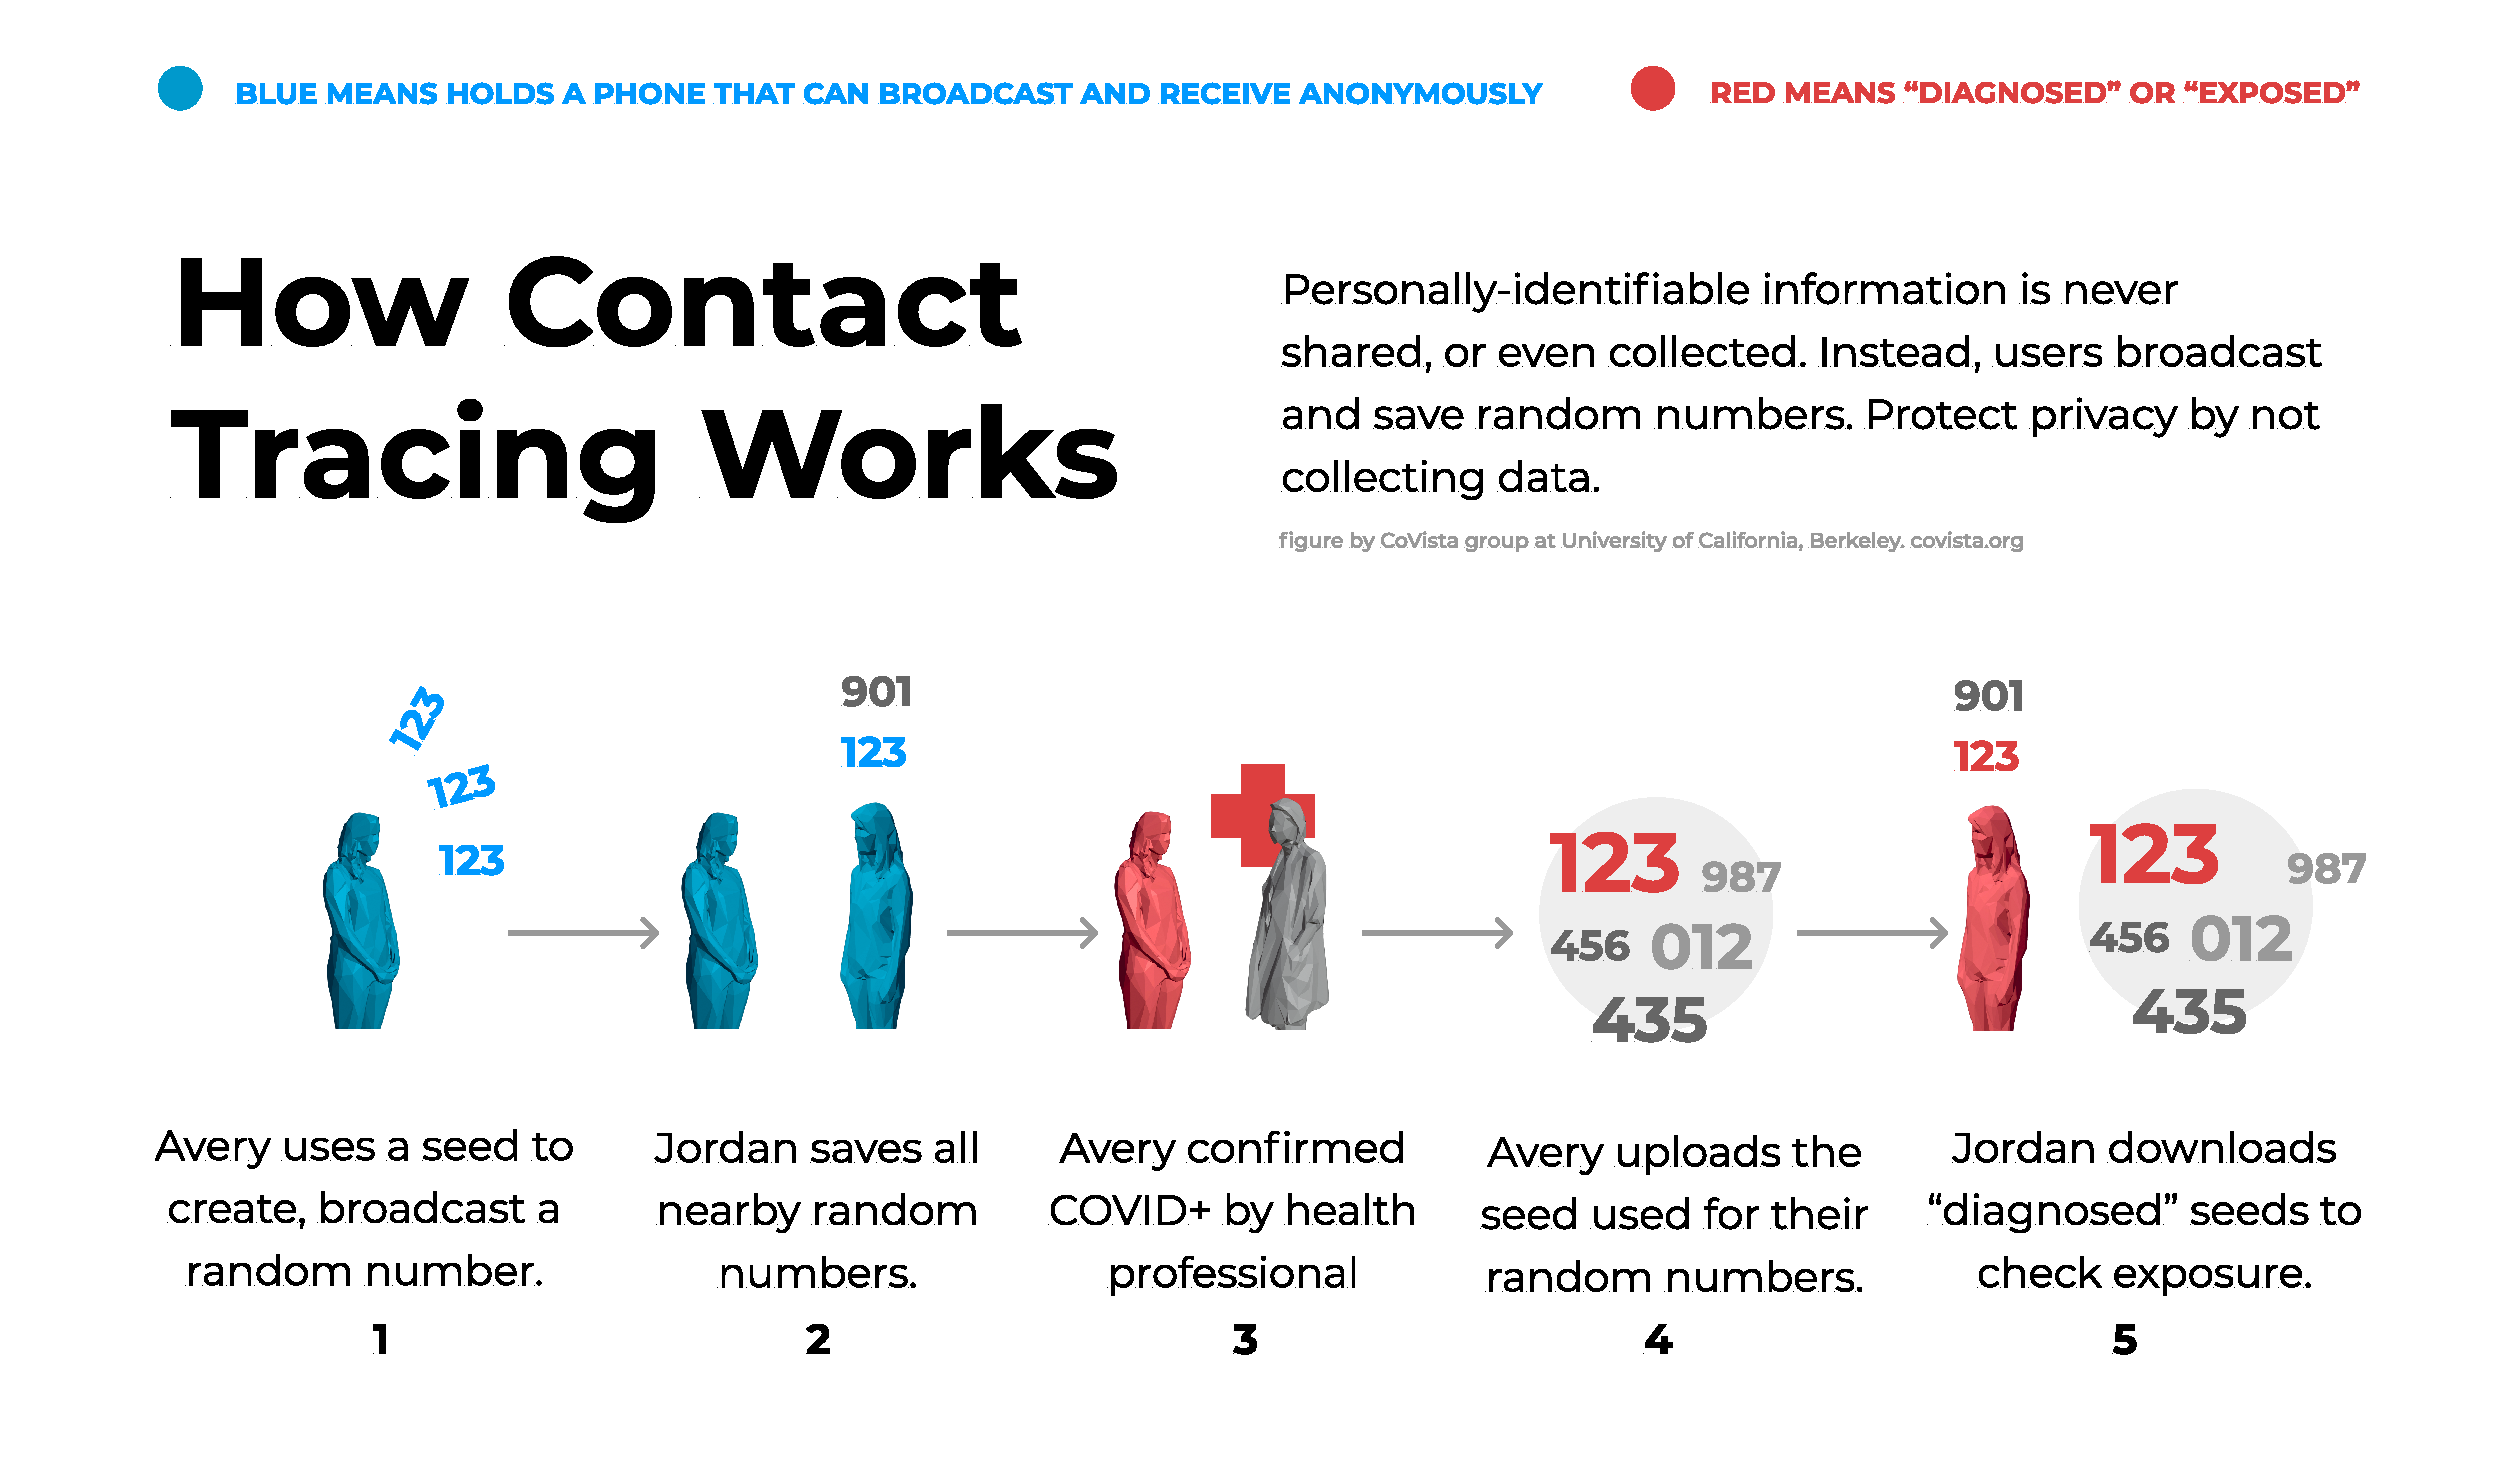
\includegraphics[width=0.8\textwidth]{figs/how_contact_tracing_works.pdf}
    \caption{Apple-Google Exposure Notification (AGEN) Protocol Overview.}
    \label{fig:contact_tracing}
\end{figure}

Governments and public health authorities want to understand where and how the disease is spreading, so they can take preventative measures.  
They also want to be able to use mobile contact tracing to augment existing manual contact tracing efforts.
With these goals in mind, governments advocate for a centralized approach, whether national or regional, where they maintain records of each person’s locations and interactions. 
This allows governments to determine exposures and notify people directly, as timeliness reduces spread. 
While centralized contact tracing may offer utility critical to re-opening the world’s economy, it raises profound concerns for civil liberties and personal privacy.
Government efforts that avoid reliance on the industrial Exposure Notification offerings have run into a host of failings, including reliability, power drain, interoperability, and participation.

Apple and Google have taken an unprecedented position -- essentially dictating public policy, not just by requiring the decentralized approach, but also by prohibiting contact tracing apps from collecting location information.
Further, they are restricting access to the new contact tracing APIs to national governments and permitting only one app per country or region. 
This decision circumvents the local governments, tribal organizations, and community health services that are often most aware of existing manual contact tracing efforts and the needs of their communities.  
Meanwhile, government contact tracing apps have failed due to restrictions imposed by AGEN.

In this article, we present two simple measures that enable the AGEN protocol to support manual contact tracing efforts, provide visibility into the spread of disease, and return authority to local communities all while preserving privacy within the Apple and Google framework. 
\begin{enumerate}
\item \textbf{Treat places as people.} Endow public places with the same privacy-preserving technology used to monitor exposure for individuals.
\item  \textbf{Nation-scale data, not apps and processes.} Build a common backend for the AGEN protocol that spans apps and governmental boundaries.
\end{enumerate}

In the rest of this article, we describe these two simple measures and how they both improve contact tracing while also preserving individual privacy.

\subsection*{Lighthouse: Treat Places as People}
\begin{figure}[h]
    \centering
    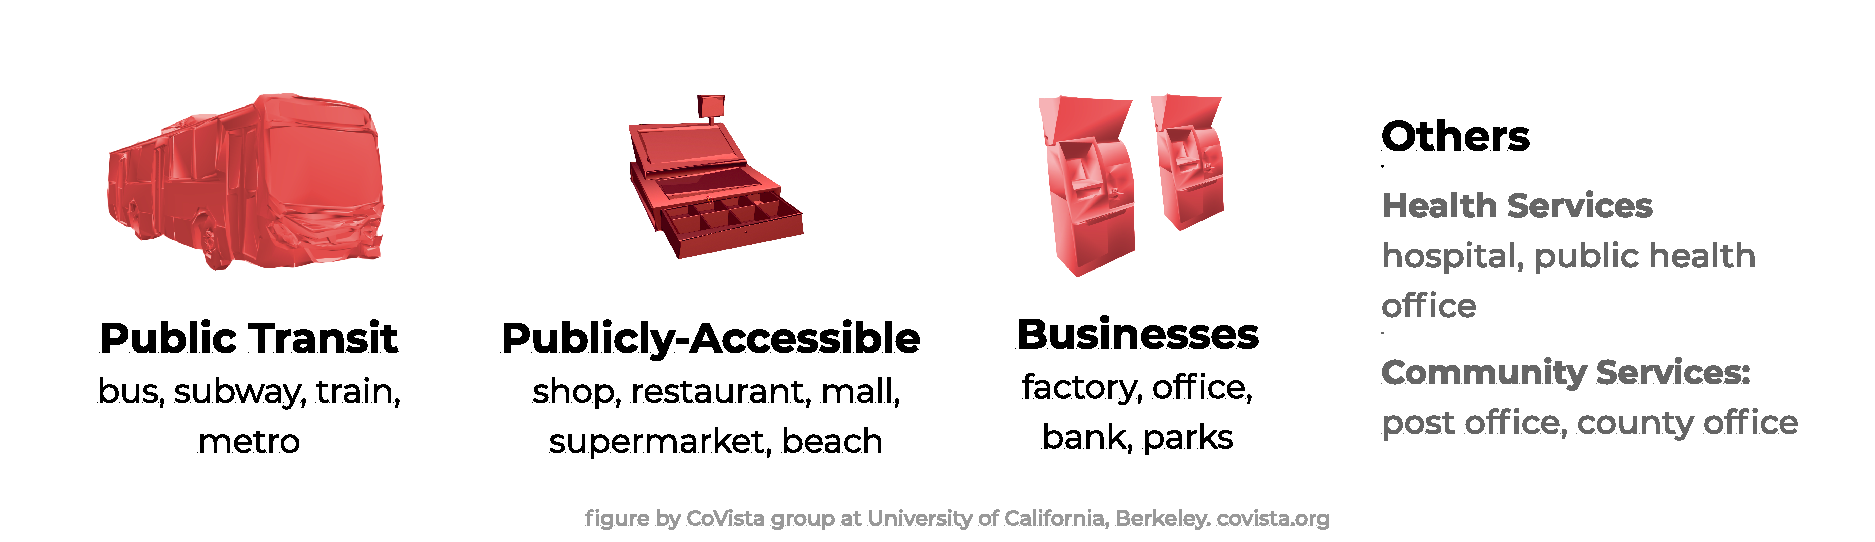
\includegraphics[width=\textwidth]{figs/places.pdf}
    \caption{Lighthouses can extend the AGEN protocol to physical places}
    \label{fig:placesExamples}
\end{figure}

If we treat public places as people, we can use the AGEN protocol to (a) understand COVID-19 exposures across space, (b) integrate with manual contact tracing, and (c) do so with the same privacy-sensitive protocol. To treat places as people in AGEN, simply attach mobile phones or specialized low-cost beacons to publicly accessible places (e.g., county services, stores, buses).  
Like a lighthouse, these devices help communicate risk associated with places.  
Well-positioned, they can offer robust proximity detection, can detect their exposure, and can convey aspects the risk that represents.

By choosing to share their locally computed exposure risk with public health authorities through the AGEN protocol, owners of publicly-accessible places can aid in mitigating virus spread. 
Alternatively, if a place is identified through traditional, manual contact tracing, the place can still anonymously participate in the AGEN protocol, notifying others without revealing where they were exposed. 
Treating places as people empowers stewards of public spaces to collaborate with public health authorities to help mitigate the spread of disease without jeopardizing the privacy of patrons or the reputation of the public spaces.
This procedure can facilitate detection of exposure from a non-participating individual while improving anonymity over manual contact tracing methods.  Going even further, such places could provide other means of beaconing that do not involve smartphones, such as QR code displays, codes on receipts and so on.

\subsection*{COVID Commons: A Nation-scale Data Backend}

Rather than “one app per nation,” a better solution would be to provide a common privacy-preserving data exchange across apps and administrative boundaries — a Commons.  This would allow societal structures and innovation, rather than corporate policy, to determine how the app ecosystem should evolve.  It is very likely that participation will be greatest if the apps are available through local organizations (e.g., tribal organization, university campus) that individuals trust.   A common privacy-preserving data exchange is already compatible with the AGEN protocol.

\begin{figure}[h]
    \centering
    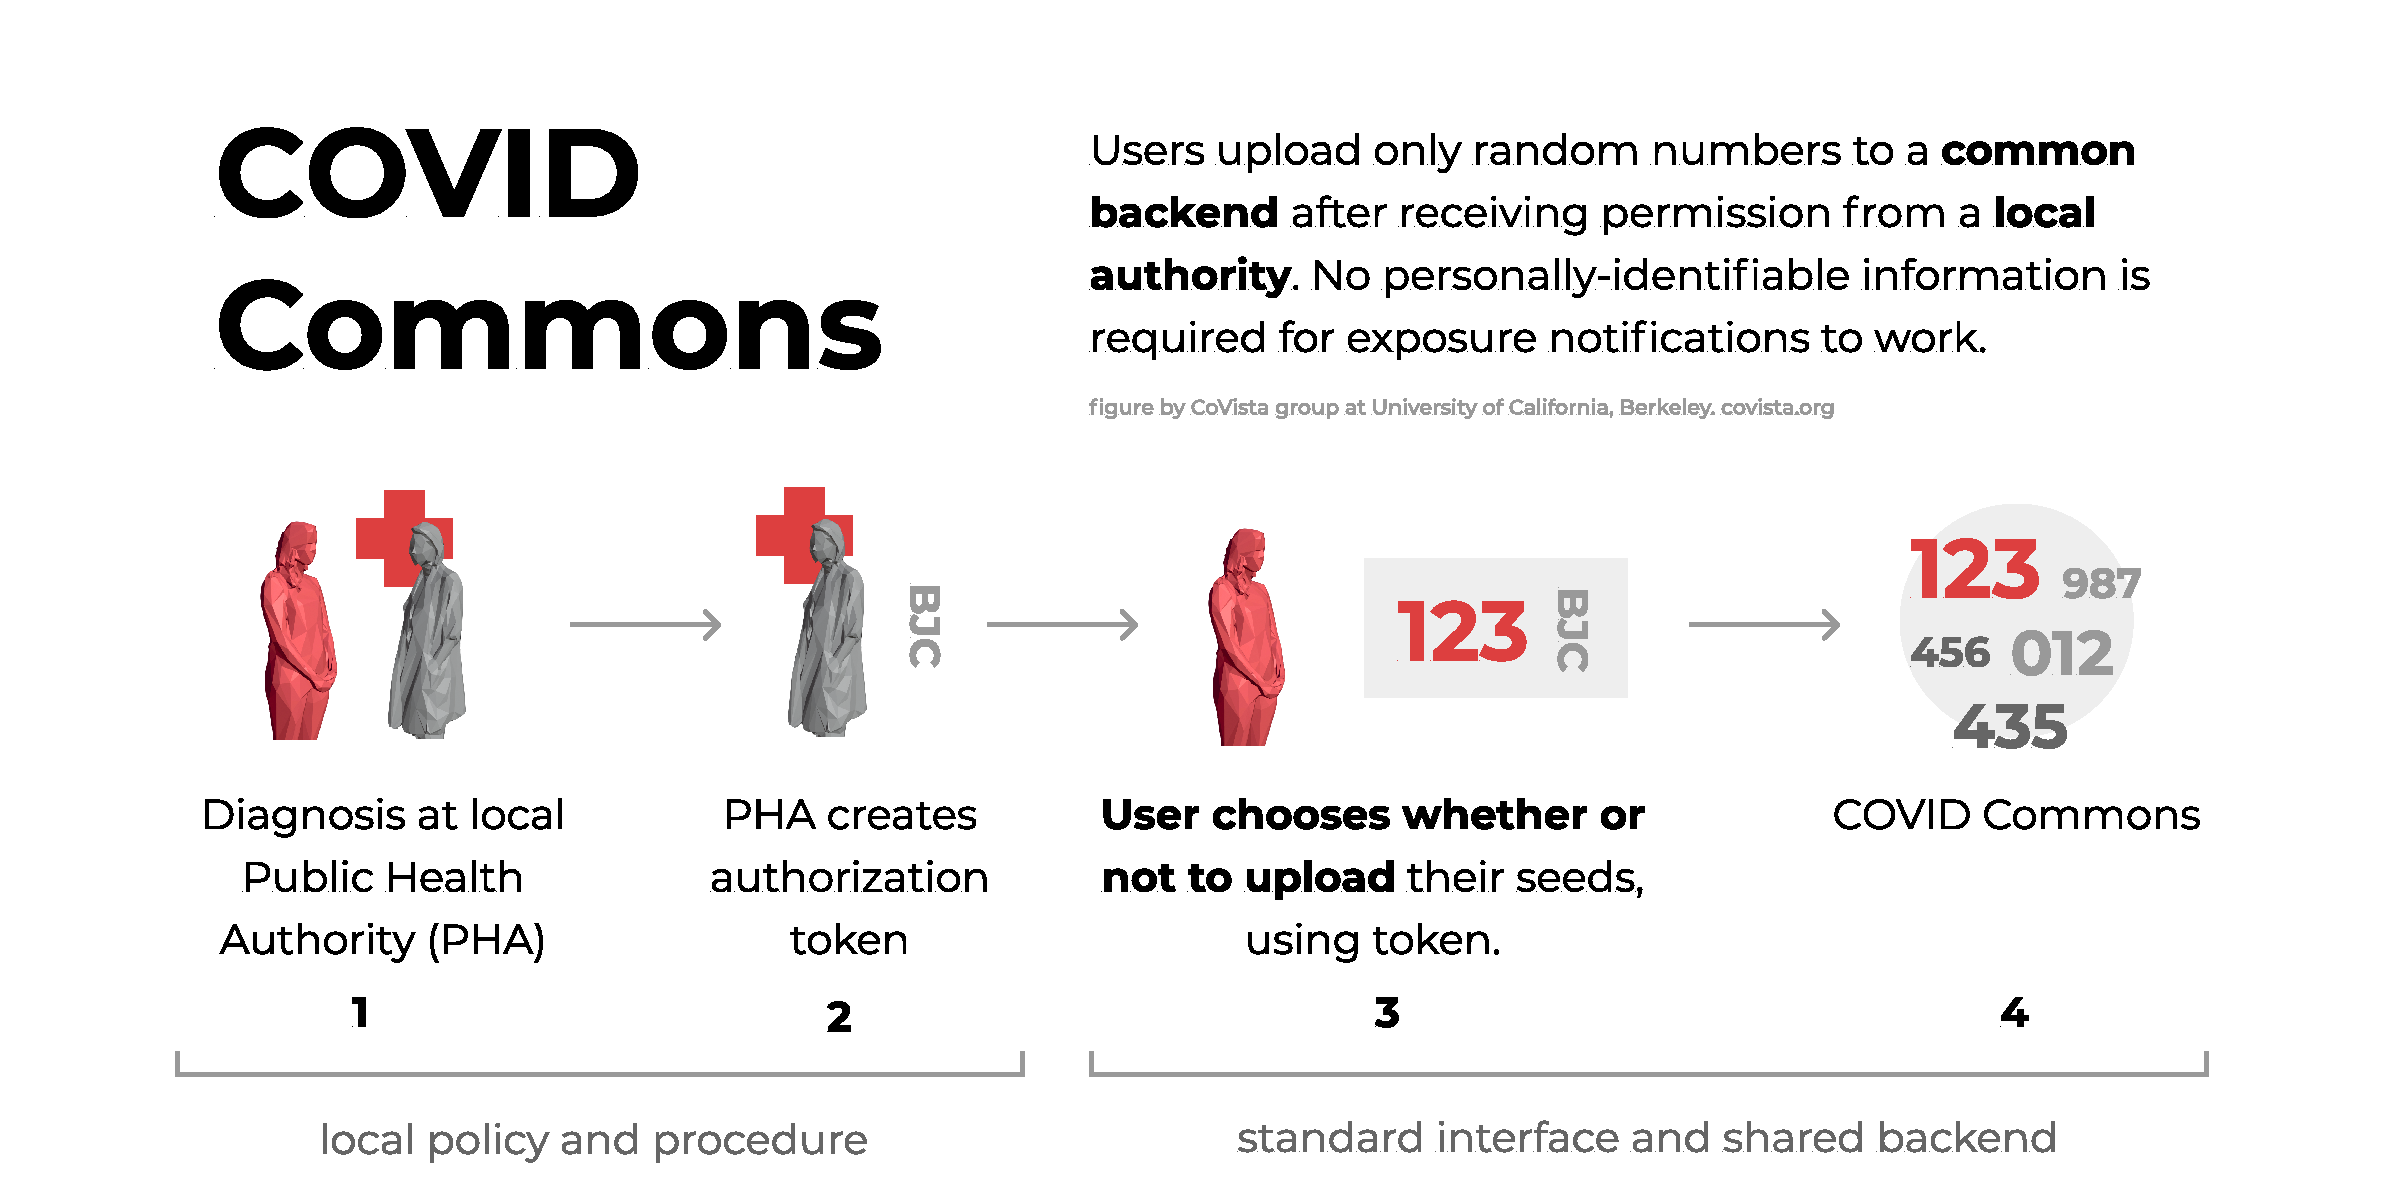
\includegraphics[width=\textwidth]{figs/covid_commons.pdf}
    \caption{Covid Commons exposure notification process.}
    \label{fig:commoms}
\end{figure}

When an individual tests positive and they engage in a conventional contact tracing interview with a public health professional. The professional obtains an authorization so the individual, on an opt-in basis, can share their anonymous exposure information.  Public health professionals serve to protect the integrity of the information in the Commons without exposing any patient data or medical data. \shankari{individual obtains authorization from professional. "an authorization"? is something like "token" missing?}

Their actions are quite similar to publishing counts of cases, statistics and demographic information, as is done today.  The Commons might be hosted by governmental or NGO structures, based on national or regional policy.  A diverse and innovative app ecosystem can grow to meet the needs of individuals and agencies.

In the remainder of this article we describe both these technical solutions in greater detail.  
We have organized each section to be relatively self-contained.

\vspace{-0.2in}
\section{Data Model}\label{dm}
\vspace{-0.1in}
We introduce different variables and characterize human factors~\cite{hf1,motiv00,motiv0,motiv1,motiv2,motiv3,motiv4}. A crowdsourcing platform typically comprises of workers and tasks that serve as the foundation of the framework we propose. We also note that not all the variables are pertinent to every application domain (for example, citizen science applications are usually voluntary contributions). Our effort is to propose a generalization nevertheless. 

{\bf Domains/types:} A set $D=\{d_1,d_2,\ldots,d_{l}\}$  of given domains is used to describe the different types of tasks in an application. Using Example~\ref{ex1}, a particular species may construe a domain. 

{\bf Workers:} A set of $m$ human workers $\mathcal{U}=\{u_1,u_2,\ldots,u_m\}$ are available in a crowdsourcing platform.
% Each worker $u$ is described by a set of  {\em human factors}~\cite{hf1,motiv00,motiv0,motiv1,motiv2,motiv3,motiv4}, i.e., variables that are important to understand their behavior in a crowdsourcing platform.

{\bf Tasks and sub-tasks:} A task $\mathcal{T}$ is a hybrid human-machine computational task (classification for example), with a quality condition $Q^\mathcal{T}$  and an overall monetary budget $B^\mathcal{T}$ that decide its termination. Using Example~\ref{ex1}, $\mathcal{T}$ is a classification task which terminates, when $Q^\mathcal{T} = 80\%$ accuracy is achieved, or $B^\mathcal{T} =\$100$ is exhausted.

Without loss of generality, $\mathcal{T}$  comprises of a set of $n$ subtasks, i.e., $\mathcal{T} =\{t_1,t_2,\ldots,t_n\}$. These sub-tasks are of interests to us,  as workers will be involved to undertake these sub-tasks. Each sub-task can either be performed by human workers or computed (inferred) by machine algorithms. We consider {\em pool based active learning}, where a finite pool of sub-tasks exists and given.

{\em Sub-tasks:}
For single label, a sub-task is an unlabeled instance of the data that requires labeling. Considering Example~\ref{ex1}, this is analogous to confirming the presence or absence of a species in a particular geographic location. 
%To generalize, we consider similar settings as that of {\em pool-based active learning}, where a pool of unlabeled instances are available for further labeling.
For multi-label scenario, a sub-task requires multiple labels to be obtained. Using Example~\ref{ex1}, this is analogous to obtaining Kingdom, Phylum, Class, Order, etc of the insect.

{\bf Worker Response:} We assume that a worker $u$'s {\em response to a particular sub-task $t$ may be erroneous, which is used by the machine algorithm in one or more rounds of interactions}. Our framework may ask multiple workers to undertake the same task to reduce the error probability, and may decide which questions to ask in the next round to whom based on the answers obtained in the previous round.

{\bf Human Factors:} These are the variables that characterize the behavior of the workers  in a crowdsourcing platform~\cite{hf1,motiv00,motiv0,motiv1,motiv2,motiv3,motiv4}.

{\em Skill (Expertise/Accuracy):}  Worker's skill in a domain is her expertise/accuracy. Skill of a worker in a domain $d$ is quantified in a continuous $[0,1]$ scale (to allow a probabilistic  interpretation). A worker $u$ may have skills in one or more domains (e.g., different species observation accuracy). 
%Given $l$ domains, $u$'s skill is described by a $l$-dimensional vector, where $s^{u_i}$ is her skill in the $i$-th domain. 

{\em Wage:} A worker $u$ may have a fixed wage $w_u$, or may have to accept the wage a particular task offers. $u$'s may have different wage for different types of tasks.

{\em Motivation:} Motivation aims at capturing the worker's willingness to perform a task. A related work~\cite{motiv1} proposes a theoretical foundation in motivation theory in crowdsourcing platform and characterizes them in two different ways: 

{\em (a) Intrinsic motivation:} Intrinsic motivation exists if an individual works for fulfillment generated by the activity (e.g. working just for fun). Furthermore, related works~\cite{motiv1,motiv2,motiv3} have identified that intrinsic motivation emerges in the following ways: (1) skill variety (refers to the extent to which a worker can utilize multiple skills), (2) task identity (the degree to which an individual produces a whole, identifiable unit of work, versus completion of a small unit which is not an identifiable final product), (3) task significance (the degree to which the task has an influence over others), (4) autonomy (the degree to which an individual holding a job is able to schedule his or her activities), (5) feedback (the extent to which precise information about the effectiveness of performance is conveyed). 

%Hackman and Oldham~\cite{hackman1976motivation} have combined these factors mathematically and defined {\em motivating potential score (MPS)} to capture intrinsic motivation:

%\begin{equation}\label{eqn}
%\begin{aligned}
%MPS= \frac{\text{skill-variety} + \text{task-identity} + \text{task-significance}}{3}  \\
%* \text{ autonomy } * \text{ feedback}
%\end{aligned}
%\end{equation}


{\em (b) Extrinsic motivation:} Extrinsic motivation is  an instrument for achieving a certain desired outcome (e.g. making money).

%{\em Acceptance ratio:} Acceptance ratio describes the {\em probability} at which a worker actually participates in a task (notice that a worker can always decline a task).Acceptance ratio may be correlated to worker motivation.
 %Given $l$ domains, $u$'s acceptance ratio is described by a $l$-dimensional vector $A^u$. 

The challenge however is, either the values of these factors have to be explicitly given or they have to be estimated. Related works, including our own, have proposed solutions to estimate skill~\cite{skill,DBLP:conf/kdd/JoglekarGP13} by analyzing historical data. %Acceptance ratio or wage of the workers are estimated by designing surveys and asking explicit questions~\cite{roy2015task}.
Nevertheless, we are not aware of any effort that models motivational factors or design optimization involving them.

{\em Worker specific constraints:} Additionally, a worker may specify certain constraints (e.g., can not work more than $6$ hours, or travel farther than $10$ miles from her current location).

{\bf Characterizing sub-tasks considering human factors:}  It is easy to notice that the motivational factors described above are actually related to tasks (i.e, sub-tasks). 

Formally, we describe that a set $A$ of attributes or meta-data is available to characterize each sub-task $t$. They are its required skill-domain\footnote{\small for simplicity, we assume that each sub-task requires one skill, whereas, in reality, multiple skills may be needed for a sub-task. The latter assumption is trivially extensible by our framework.} $s^t$ , cost/wage $w^t$, duration $time^t$, location $location^t$, significance $sig^t$, identity $iden^t$, autonomy $auto^t$, task feedback $fb^t$. Each $t$, if performed correctly, contributes by a quantity  $q^t$ to $Q^\mathcal{T}$. These contributions are purely dictated by the active learning principles, such as how much it reduces the uncertainty.



%{\em Unlike other human factors, there does not exist any mathematical model that captures human motivation}. We therefore make an effort to mathematically model human motivation. 

 %and has a cost $b^t$. The cost of a sub-task is the money that has to be paid when it is performed by a human worker.

 







\vspace{-0.2in}
\section{Worker-Centric Optimization through Human Factors Modeling}\label{hf}
\vspace{-0.1in}
Recall Section~\ref{intro} and note that worker-centric optimization is a common theme across single and multi-labels tasks, which we first examine here.

{\bf Objectives:}
Our objective here is to explore mathematical models for worker-centric optimization in crowdsourcing platforms. Specifically, given an available pool of tasks and workers where workers perform repetitive tasks, we first obtain human factors of the workers by analyzing their past tasks and then study the problem of task assignment to enable worker-centric optimization. A recent work performs an ethnomethodological study at {\em Turker Nation}\footnote{\small http://www.turkernation.com/} and argues~\cite{martin2014being} that it is critical to enable worker-centric optimization.
Our effort here is to make a formal step towards that goal, independent of any specific system-centric optimization (i.e., the active learning principles). Therefore, such a study has a much broader applicability that goes beyond active learning. Of course, our framework will ultimately combine both system and worker-centric criteria. 

 {\bf Challenges:} While the significance of human factors is well-acknowledged in crowdsourcing, the challenge is to be able to estimate them effectively and propose appropriate models that could capture them during task assignment. Added to the fact is the dependence of the underlying crowdsourcing domain, which makes some of these factors more important than the rest (e.g., unlike AMT, there is no monetary pay-offs in citizen science activity, but skill variety is acknowledged to be critical to avoid monotony). 

%{\bf Our Prior Work:} In our recent investigation, we have studied some human-factors, such as, worker skill (accuracy), wage (pay-off), acceptance ratio of tasks, social affinity~\cite{hf1,roy2015task,DBLP:journals/corr/RahmanRTAD15} and proposed mathematical functions to include them explicitly in task assignment. We have designed medium-scale user studies~\cite{roy2015task,DBLP:journals/corr/RahmanRTAD15} in Amazon Mechanical Turk (AMT), involving hundreds of workers to learn the relationship between these factors and have observed that skill, wage, acceptance ratio - all follow normal distributions. We also have observed that a strong positive correlation exists between worker accuracy and expected wage. These studies have demonstrated empirically that task assignment considering human factors yields superior outcomes compared to the one without. In another recent work, we present how to combine task relevance (Boolean match of worker's expertise with the skill requirements of the tasks) and motivation in the task assignment process~\cite{edbt172}, albeit in a non-active learning context. Moreover, this work only considers {\em skill-variety} in formalizing motivation. In that sense, this latter work is still preliminary and does not solve the problem we propose. A recent survey paper summarizes different aspects of worker centricity in crowdsourcing platforms~\cite{amer2016toward}. 


\vspace{-0.1in}
\subsection{Proposed Directions}
\vspace{-0.1in}
First, we propose how to model and estimate human factors~\cite{hf1,motiv00,motiv0,motiv1,motiv2,motiv3,motiv4} that are pertinent to capture motivation using the variables that are described in Section~\ref{dm}. Then, we describe mathematical models that leverages these estimated human factors to explicitly assign tasks to workers. 

{\bf Estimating human factors:} We leverage the past task completion history of the workers as well as the new tasks to compute a Boolean task completion matrix $T$, where the rows are the workers and the columns are the (sub)-tasks. If a worker $u$ has completed a (sub)-task $t$ successfully in the past, the corresponding entry gets a $1$, it gets a $0$ otherwise. We assume that the factors that capture intrinsic motivation, i.e., skill variety, task identity, task significance, autonomy, feedback are independent yet latent variables. The second matrix we consider is the task factor matrix $\mathcal{F}$, where the rows are the tasks and the columns are the motivation related latent variables.  The final matrix is the user factor matrix $\mathcal{U}$ where rows are the factors and columns are the users. This matrix could be fully latent or observed.  In case it is latent, we minimize the error function, as defined below:

\begin{equation}
\sum_{i,j}(t_{ij}-\mathcal{U}_iF_j)^2+\lambda(\|\mathcal{U}\|^2+ \|\mathcal{F}\|^2)
\vspace{-0.1in}
\end{equation}

Here, $\lambda$ is the regularization parameter. The goal is to find ${\mathcal U}$ and ${\mathcal F}$ such that it minimizes the error. For any new worker and new task, the predicted task completion score is calculated by multiplying $U_i$ with $F_j$. Here, the important thing is to notice that the optimization function only minimizes the error for which ratings are present.  We apply the alternating least square approach~\cite{stigler1981gauss} to solve this problem. This is an iterative approach, where at each iteration, we fix the tasks' latent factor matrix $\mathcal{F}$ in order to solve for $\mathcal{U}$ and vice versa. We have designed a similar solution for predicting tasks to workers considering implicit workers' feedback\cite{DBLP:journals/corr/RahmanJR16}.

 
{\bf Worker-Centric Task Assignment:} The solution above only estimates the intrinsic motivational factors, but does not describe how to aggregate them together or combine with extrinsic motivation to perform worker-centric task assignment. 

Psychologists Hackman and Oldham~\cite{hackman1976motivation} have combined factors associated to intrinsic motivations defined {\em motivating potential score (MPS)} :

\begin{equation}\label{eqn}
\begin{aligned}
MPS= \frac{\text{skill-variety} + \text{task-identity} + \text{task-significance}}{3}  
 *\text{ autonomy } * \text{ feedback}
\end{aligned}
\end{equation}

Considering this aforementioned formulation, we study the worker-centric task assignment as a global optimization problem to maximize the {\em aggregated intrinsic and extrinsic motivation}. For a given set of tasks $S^{t_u}$,  $V(S^{t_u})$ represents the overall motivation for worker $u$, by combining  her extrinsic motivation  (EXTM) (recall Section~\ref{dm} that EXTM could be modeled using wage $w^t$) and intrinsic motivation, i.e, {\em motivating potential score (MPS)}(refer to Equation~\ref{eqn})~\cite{hackman1976motivation}. In our initial effort, we combine them linearly, as that allows us to design efficient algorithms. Assigning a set of tasks per worker is reasonable as well as desirable from worker's perspective, because workers in a typical crowdsourcing platform intend to undertake multiple tasks as opposed to a single task. Workers may also have constraints, such as,  not spend more than $X^u$ hours, 
or the aggregated wage must at least be $b^u$ dollars. 
 
Technically, we want to assign tasks to the workers {\em to maximize the aggregated motivation, such that the assignment satisfies each worker-specific constraints}. One such optimization function is described in Equation~\ref{eqn:eq3} (Recall Section~\ref{dm} where $time^t$ and $w^t$ are the duration and wage of sub-task $t$, respectively).

\begin{equation}\label{eqn:eq3}
 \text{ Maximize }  \sum_{u \in \mathcal{U}} [V(S^{t_u}) =  EXTM(S^{t_u}) + MPS(S^{t_u})]
\end{equation}
\vspace{-0.2in}
\begin{align*}
 V(S^{t_u}) =
\begin{cases} 
 \\ \text{ if } \sum_{t \in S^{t_u}} time^t \leq X^u \text{ and } \sum_{t \in S^{t_u}} w^t \geq b^u \\
0 \text{\qquad otherwise} 
\end{cases}
\vspace{-0.1in}
\end{align*} 


%Recall that a task $t$ is associated with a set $A$ of attributes, whose values, we assume are provided by the domain experts and are available at our disposal. Formally, for each task, we know the required skill domain $s^t$, duration $time^t$, significance $sig^t$, identity $iden^t$, autonomy $auto^t$, feedback $fb^t$, and wage $w^t$.

As a simple example, given two tasks $i$ and $j$, we can add the individual significance $sig^i+sig^j$, identity $iden^i+iden^j$, autonomy $auto^i+auto^j$, or feedback $fb^i+fb^j$. Similarly, the  wage of two tasks could also be added and normalized to compute EXTM. 
Alternative problem formulation is explored below.
%However, in order to compute MPS,  we still need to model and quantify the {\em skill variety} of a given set of tasks. 

%{\em Modeling Skill-variety:} We intend to study two different ways to capture skill variety. 

%(1) Set based modeling: Simple set based measures, such as, {\em Jaccard Distance}~\cite{baeza1999modern} can  be used to quantify {\em skill variety} between a given set of tasks. As an example, given $2$ tasks $t_1,t_2$ from citizen science, if $s^{t_1}=\text{humming bird}$, $s^{t_2}=owl$, skill variety $skill-variety(t_1,t_2)=1$. 

%In some application, it is reasonable to assume that an {\em intrinsic diversity ordering}~\cite{vee2008efficient} between the task attributes are available which can potentially be used to quantify skill-variety. For example, two sub-tasks associated with the same location that require to observe two different species may require more skill variety than two other sub-tasks that require observing the same species but from two different locations. We formalize this as, $\text{skill-domain} \prec \text{location}$. If such a diversity ordering is available from the domain experts, we model skill-variety considering diversity ordering~\cite{vee2008efficient}.

%(2) Order based modeling: An interesting alternative of the set based skill-variety computation  is to design an {\em ordering based}~\cite{DBLP:conf/icde/RoyDAY11,cao2012keyword} solution, where a {\em chain} of sub-tasks will be designed for a worker. Using Example~\ref{ex1}, this would mean creating an ordering $\mathcal{R}$ of the tasks for each worker where the skill-variety is ideally very high. Unlike set based approaches, here, skill-variety of a given set of sub-tasks will be computed considering each $k$ adjacent sub-tasks in the designed chain ($k=2$ means pair-wise adjacent tasks). As a simple example, if $3$ sub-tasks $t_2 \rightarrow t_1 \rightarrow t_3$ are designed for a worker, for $k=2$,  $skill-variety(t_2 \rightarrow t_1 \rightarrow t_3)= Jaccard(s^{t_2},s^{t_1})+ Jaccard(s^{t_1},s^{t_3})$.  %This modeling could also be extended when diversity based ordering between the attributes are available.


%The directions described above give rise a number of interesting computation problems.

%MPS formula requires us to quantify {\em skill variety} for a given set of tasks. We note that modeling skill variety leads to interesting research problems. Additionally, how to solve the objective function described above efficiently remains to be a challenging problem.
\vspace{-0.1in}
\subsection{Open Problems}
\vspace{-0.1in}
 {\bf  Solving the optimization problem:}
How to design an effective solution to maximize worker motivation based on the aforementioned objective function formulation is challenging. %The problem becomes even more complex when skill-variety is modeled as a chain. Even when set based modeling is considered, 
We observe that the proposed optimization problem is NP-hard~\cite{garey1979computers}, using a reduction from the assignment problems~\cite{roy2015task}. In a recent work, we have modeled motivation using {\em only skill-variety} and we have proved that the problem is NP-hard using a reduction from the Maximum Quadratic Assignment Problem~\cite{arkin2001approximating}. For our problem, we note that an integer programming based solution is simply not scalable. We will explore greedy heuristic strategies that are effective and efficient. For example, we will assign tasks to the workers greedily based on the marginal gain~\cite{roy2015task}. 
%if the set-based formulation admits {\em sub-modularity}~\cite{lovasz1983submodular}, as {\em skill-variety} exhibits {\em diminishing return properties}, and other motivational elements simply increase as more tasks are added. If this property is indeed satisfied, we will be able to design greedy approximation algorithms~\cite{nemhauser1978analysis} with theoretical guarantees. For the ordering based model, we will explore orienteering like solutions~\cite{chao1996fast} to design efficient greedy heuristic algorithms.

\noindent {\bf  Complex modeling for estimating intrinsic motivation \& task assignment:} In our preliminary direction, we have assumed that variables associated with intrinsic motivations are independent and could be combined as suggested by Hackman and Oldham~\cite{hackman1976motivation}, or intrinsic and extrinsic motivation could be combined linearly. In reality, that may not be the case. In this open problem, we will study the feasibility of a probabilistic model~\cite{zhao2012bayesian}, namely a {\em hierarchical Bayesian framework}~\cite{liu2014framework} for this problem. If the worker is completely new in the platform, we will bootstrap to collect a small set of evidence. We will consider each of the variables associated with worker motivation as a random variable and present a model using hierarchical Bayesian Networks~\cite{jensen1996introduction} by encoding a joint distribution of these variables over a multi-dimensional space.  This model will first establish the relationship among the intrinsic motivational variables themselves and then between intrinsic and extrinsic motivation to capture a workers' ``preference'' to a given task. We will apply Constraint Based, Score-Based, and Hybrid methods to learn the structure of the network~\cite{tsamardinos2006max}. We will leverage {\em Bayesian Parameter Estimation as well as Maximum Likelihood Estimation techniques} to learn the parameters of the constructed network. For efficient parameter estimation considering this complex joint distribution, we will use Gibbs sampling~\cite{carter1994gibbs}. 

%As outlined in the aforementioned open problem, if we are successful to model the motivational variables using a graphical model through probabilistic modeling, we shall extend that model to a hierarchical Bayesian Network with constraints that 

%In our preliminary work, we have assumed that variables associated with intrinsic motivation are combined as suggested by Hackman and Oldham. Moreover, we have aggregated intrinsic and extrinsic motivation linearly, as described in Equation~\ref{eqn:eq3}. In this open problem, we will explore alternative modeling. 






\vspace{-0.2in}
\subsection{Optimized Single-Label Acquisition Involving Crowd}\label{label}
\vspace{-0.1in}
We now investigate our proposed optimization framework for single-label acquisition. This problem is examined by augmenting active learning principles with worker-centric optimization (refer to Section~\ref{hf}).

{\bf Objectives:} We are assuming a setting where single-label acquisition is difficult, expensive, and time consuming (such as, Example~\ref{ex1}). We adapt a set of popular as well as well-known active learning principles\cite{al1,qbc1,qbc2,error-reduction} that are proposed to optimize system-centric cirteria, such as, {\em minimizing uncertainty or maximizing expected error-reduction} that are known to be effective in supervised (classification) algorithms~\cite{al-svm,al-svm2,al-dtree,korner2006multi}. We augment these active learning principles with worker-centric optimization. Given a pool of unlabeled instances  (of sub-tasks) and an available set of workers, the objective is to select sub-tasks for further labeling and assign workers for annotations, such that, the assignment optimizes both system and workers. The same sub-task may be annotated  by multiple workers.

{\bf Challenges:} An oracle, who knows the ground truth, no longer exists in crowdsourcing; instead, multiple workers, with varying expertise (skill), are available. Under this settings, how to realign traditional active learning goals that are system-centric (i.e., optimizes underlying computational task) requires further investigations. How to systematically design {\em optimization function}, i.e., one that combines worker-centric optimization in traditional active learning settings~\cite{active-learning-cs1,active-learning-cs2} is the second important challenge. An equally arduous challenge is the efficiency issue which is mostly overlooked in the existing research. Finally, when to terminate further label acquisition also needs to be examined.

\vspace{-0.1in}
\subsection{ Proposed Directions}
\vspace{-0.1in}
Our overall approach is iterative, where, in each round a set of sub-tasks are selected for annotation and a set of workers are chosen. Once annotations are received, the underlying classification model is retrained. After that, either the process terminates or we repeat. It has three primary directions: (1) {\em in a given round, which sub-tasks are to be selected for annotation and assigned to which workers?} (2) {\em  how to aggregate multiple annotations to obtain the ``true'' label?} (3) {\em when to stop?}  

{\em Which sub-tasks are to be selected and assigned to which workers?} We take a set of well-known active learning techniques, such as, {\em uncertainty sampling \cite{al1}, query-by-committee \cite{qbc1,qbc2}, or expected-error reduction~\cite{error-reduction}, used in popular classification algorithms, such as, Naive Bayes~\cite{entropy}, SVM~\cite{al-svm,al-svm2}, Decision Trees~\cite{al-dtree}, or ensemble classification\cite{korner2006multi}} and study them in crowdsourcing.

When a single classifier with a binary classification task is involved and the classifier is probabilistic (such as Naive Bayes), we consider existing uncertainty sampling~\cite{al1} techniques. We use entropy~\cite{entropy} to model uncertainty to choose that sub-task for labeling whose posterior probability of being positive is closest to $0.5$. For non-probabilistic classifiers (such as SVM or Decision Tree), we explore {\em heterogeneous approach}~\cite{lewis1994heterogeneous}, in which a probabilistic classifier selects sub-tasks for training the non-probabilistic classifier. We also study existing expected-error reduction~\cite{error-reduction} techniques that select the sub-tasks to minimize the expected future error of the supervised algorithm, considering {\em log-loss or $0/1$-loss}. We study the query-by-committee\cite{qbc1,qbc2} technique, we choose that sub-task for further labeling which has the {\em highest disagreement}. 

Active learning principles  mentioned above are too {\em ideal} to be useful in a crowdsourcing platform. A simple alternative is to design a {\em staged solution}, where we first select the tasks and then the workers~\cite{active-learning-cs1}. For us, we can take the task-selection solution from~\cite{active-learning-cs1} and then plug in our worker-centric optimization (Section~\ref{hf}) to compose tasks for the workers. We, however, argue that such a staged solution is {\em sub-optimal}, simply because, tasks selected by {\em active learning} techniques may end up having a very low worker-centric optimization, resulting in poor outcome overall. We therefore propose a global optimization that combines (1) worker-centric goals (recall Equation~\ref{eqn:eq3}). (2) active learning principles considering workers with varying expertise. 

Recall Section~\ref{dm} and note that $q^t$ represents sub-task $t$'s contribution towards a given active learning goal (for example, how much $t$ reduces uncertainty or expected-error) at a given iteration. Let $S^{t_u}$ represent the sub-tasks assigned to $u$ with value 
$V(S^{t_u})$ (recall Equation~\ref{eqn:eq3}). Considering worker's skill $s^{u_t}$ as a probability, $u$'s {\em expected contribution} to $t$ is  $s^{u_t} * q^t$~\cite{clemen2007aggregating}. One possible way to combine them is as a multi-objective global optimization function where the objective is to select sub-tasks and workers that maximize a weighted linear aggregation of worker and task-centric optimization (Equation~\ref{eqn:eq2}, where $W_1,W_2$ are specific weights). While linear aggregation is not the only way, it is more likely to admit efficient solutions, where the weights are tunable by domain experts (by default, $W_1=W_2=0.5$). 


%In our initial direction, we combine them in a weighted linear fashion  considering weights by combining both worker and task-centric criteria, where the latter is modeled as a linear weighted aggregation by multiplying $q^t$ with $s^{u_t}$ ($u$'s skill/accuracy in task $t$).

\begin{equation}\label{eqn:eq2}
 \text{ Maximize } \mathcal{V} =  \sum_{u \in \mathcal{U}} [W_1 * V(S^{t_u}) +  W_2 * \sum_{t \in S^{t_u}} (s^{u_t}*q^t)]
\end{equation}

Additionally, if a task has a cost budget associated that could be assigned either as a constraint to this optimization problem, or we could use cost as another objective as part of the optimization function, akin to one of our recent works~\cite{roy2015task}. Nevertheless, we acknowledge that designing the ``ideal'' optimization model that suffices the need of every application is practically impossible. We address this in the open problems.

{\em  Aggregating multiple annotations:} Another challenge is how to combine annotations from multiple workers with varying expertise to obtain the ``true'' label. We apply weighted majority voting types of approach~\cite{ho2013adaptive}, where the weights are chosen according to the skills of the workers. We also consider iterative algorithm for this purpose. Examples of iterative techniques include EM or Expectation Maximization\cite{hung2013evaluation}. The main idea behind EM is to compute in the $E$ step the probabilities of possible answers to each task by weighting the answers of workers according to their current expertise, and then to compute in the $M$ step re-estimates of the expertise of workers based on the current probability of each answer. The two steps are iterated until convergence.  We explore Bayesian solution~\cite{clemen2007aggregating} to probabilistically obtain the true label, i.e., given workers' annotations and skill, compute $Pr(t=0)$ and $Pr(t=1)$ and choose the one which has the higher probability.

%There exists a number of complex technical open problems.
\vspace{-0.1in}
\subsection{Open Problems}\label{opp}
\vspace{-0.1in}
{\bf  Solving the optimization problem} Solving the optimization problem described above is challenging. In a very recent work, we have formalized  task assignment as a linear combination of task relevance (based on a Boolean match between worker expertise and the skill requirements of a task) and skill-diversity~\cite{edbt172} and proved the problem to be NP-Complete~\cite{feo1990class,feo1992one}. We use Maximum Quadratic Assignment Problem (MAXQAP in short)~\cite{arkin2001approximating} to design an efficient algorithm with approximation factor $1/4$. For our problem, we will examine if it is at all possible to design an objective function (perhaps as a special case) to exploit its nice structural properties, such as, {\em sub-modularity or cancavity}. Such an effort is made for active learning problems recently~\cite{hoi2006batch} without considering human workers. We will also study the possibility of staged algorithms and heuristic solutions, as described above. To make the algorithm computationally efficient, we will examine how to design incremental active learning strategies~\cite{qi2009two}, such as finding the new classification model that is most similar to the previous one, under a set of constraints. 


{\bf Complex function design and stopping condition} We note that the formulation described in Equation~\ref{eqn:eq2} is rather {\em simple} - a linear function may not be adequate to combine worker and task-centric optimization. We will explore non-linear multiplicative functions. Another possible way is to formalize this as a bi-criteria optimization problem and design pareto-optimal solution that does not require us to assign any specific weight to the individual functions~\cite{bilo2004pareto,anagnostopoulos2012online,asudeh2014crowdsourcing}.  Finally, we  will examine {\em when to terminate this iterative process}. For the overall classification task $\mathcal{T}$, when quality threshold is not reached or budget is not exhausted (these are two hard stopping conditions), we will design stopping condition by measuring the  confidence~\cite{vlachos2008stopping} of the classification model, or availability of suitable workers.

{\bf Develop a number of optimization models that are likely to cover a variety of scenarios}  We realize that what constitutes the ``ideal'' optimization model is an extremely difficult problem and highly application dependent (e.g., Which factors are important? Should we add or multiply different human factors? In the case of linear weighting, what should be the weighting coefficients?). Even a domain expert who is very knowledgeable about the specific application may not be able to shed enough light on this. We hope to develop a rich set of different models that will cover the various types of applications. This idea of developing a set of optimization models draw parallels from Web Search and Information Retrieval - where a set of alternative criteria, such as relevance, diversity, and coverage, are considered~\cite{baeza1999modern}. In our case, this is analogous to developing models that only consider workers skills/expertise, or cost, or motivation, or includes a subset of human factors that we are interested to study in this project. 
\vspace{-0.2in}
\section{Optimized Multi-Labels Acquisition Involving Crowd}\label{unlab}
\vspace{-0.1in}
We now investigate the multi-labels acquisition scenario. We are unaware of any related work that performs multi-label acquisition in an active learning settings involving crowd. Although one can transform a multi-label task to several single-label tasks, this simple approach can generate many tasks, incurring a
high cost and latency. Akin to the previous section, our effort is to design solutions that adapt a few recent active learning works~\cite{multi0,multi1,multi2,multi3} for multi-label acquisition and combine that with worker-centric optimization, described in Section~\ref{hf}.

{\bf Objectives:} We will adapt a few known active learning algorithms for multi-label classifications using Support Vector Machine (SVM), Naive Bayes, or Ensemble classifiers~\cite{multi0,multi1,multi2,multi3}. We will combine and augment them with {\em worker-centric optimization through human factors modeling}. Using Example~\ref{ex1}, this is akin to selecting the most appropriate unidentified image of the species and select the most appropriate workers to provide multiple labels. Since a task could be labeled by multiple workers, we will study how to aggregate multiple responses and infer the correct labels (truth inference problem) of a task. We will also explore the use of correlations among different labels to improve the inference quality. Finally, we will investigate the stopping condition or {\em convergence criteria}. 



{\bf Challenges:} Workers may exhibit different characteristics in multi-label tasks: a conservative worker would only select labels that the worker is certain of, while a casual worker may select more labels. To determine the multi-label tasks’ results, the key is to
devise the so-called ``worker model'' to accurately express the behavior of the worker in answering multi-labels. Furthermore, different from single-label tasks, correlations among labels inherently exist in multi-label tasks. For Example~\ref{ex1}, consider one pairwise label dependency: if the insect in the image is labeled as Papilionidae (Family name) , then it is highly probable that it also has label
Swallowtail (Sub-family name). Therefore, how to understand and leverage label correlation is another challenge. Finally, how to systematically design {\em optimization function}, i.e., one that combines worker-centric optimization in active learning settings~\cite{multi0,multi1,multi2,multi3} is the final important challenge.


%An oracle, who knows the ground truth, no longer exists in crowdsourcing; instead, multiple workers, with varying expertise (skill), are available. Under this settings, how to realign traditional active learning goals that are system-centric (i.e., optimizes underlying computational task) requires further investigations. How to systematically design {\em optimization function}, i.e., one that combines worker-centric optimization in traditional active learning settings~\cite{active-learning-cs1,active-learning-cs2} is the second important challenge. An equally arduous challenge is the efficiency issue which is mostly overlooked in the existing research. Finally, when to terminate further label acquisition also needs to be examined.

\vspace{-0.1in}
\subsection{Proposed Directions}
\vspace{-0.1in}
Our overall approach is iterative here as well, where, in each round a set of sub-tasks are selected to be annotated with multi-labels and a set of workers are chosen. Once multiple labels are acquired, the underlying classification model is retrained. After that, either the process terminates or we repeat. It has three primary directions: (1) {\em Task assignment} (2) {\em  Truth Inference, i.e.,  aggregate multiple annotations to obtain the ``true'' labels.} (3) {\em Label Correlation}.

{\em Task Assignment:} In our preliminary investigation, we have studied the active learning problem for the multi-label scenario considering the widely popular SVM classifier using the {\em Maximum-Margin Uncertainty Sampling}. Uncertainty sampling \cite{al1} is one of the simplest and most effective active learning strategies used for single-label classification. The central idea of this strategy is that the active learner should query the instance which the current classifier is most uncertain about. For binary SVM classifiers, the most uncertain instance can be interpreted as the one closest to the classification boundary by selecting the sample with the smallest classification margin. Multi-label active learning methods simply extend this binary uncertainty concept into the multi-label learning scenarios by integrating the binary
uncertainty measures associated with each individual class in independent manners, such as taking the minimum over all classes, and taking the average over all classes.

In our initial direction, given the active learning principle, we combine that with worker-centric optimization and design an objective function akin to Equation~\ref{eqn:eq2}, as described in Section~\ref{label}. Obviously, exploring alternative optimization models, or how to design a set of optimization functions that can handle a variety of scenarios, or when to stop the iterative process are additional challenges. Once we understand these challenges for the single-label acquisition problem in Section~\ref{label}, we believe they will extend for the multi-label scenarios.

{\em  Truth Inference Problem:}
The truth inference problem, i.e, how to aggregate the annotations provided by multiple workers and generate the actual set of labels requires deeper attention for the multi-label scenario. As the correct set of labels associated with each sub-task is unknown (ground-truth is unknown), the accuracy or expertise of a worker can only be estimated based on the collected answer. To model worker expertise, we compute the following two measures, {\em True Positive (TP)} and {\em False Positive (FP)}. TP is the number of labels that a worker selected correctly and FP is the number of labels she selected incorrectly. Unlike a prior work~\cite{zhao2012bayesian}, False Negative and True Negative are not relevant, if the workers annotate the labels. In the case where workers validate the given labels, these latter two measures are also relevant. Once these measures are computed, we design a worker's contingency table and calculate her expertise. After that, we design an iterative approach, which can jointly infer the correct labels associated with the tasks and the expertise of the workers.  Our iterative solution is motivated by the Expectation Maximization (EM) algorithms and comprises of the following two steps: (step 1), we assume that the worker expertise is known and constant, and infer the probabilistic truth of each object and label pair. (step 2), based on the computed probabilistic truth of each object and label pair, we re-estimate workers expertise.

{\em  Label correlation:}
Since the annotated labels of an object are not independent (Recall Example~\ref{ex1} and note that Papilionidae (Family name) and Swallowtail (Sub-family name) are highly correlated), we study how label correlations can be inferred and facilitate truth inference. In our initial direction, we leverage the existing label correlation techniques~\cite{lc1,lc2} to generate the {\em pairwise label correlations} and regard them as prior input to our problem. %Pairwise correlation is computed on a pair of labels, whereas higher order label correlations is among a set of labels. 
For example, the conditional dependency of two labels defines the probability that one label is correct for an object under the condition that the other label is correct. Capturing the higher order label correlations requires computing the joint probability which could be computationally expensive. Once label correlation is computed, we shall explore how to use that information for improved truth inference. 
 \vspace{-0.1in}
\subsection{Open Problems}
\vspace{-0.1in}

\noindent {\bf Alternative Active Learning Strategy Design}
In our initial direction, we have discussed how to adapt uncertainty sampling to design active learning strategies for SVM classifier for multi-label scenario. The average number of correct labels assigned to each instance in a multi-label data set is called its label cardinality. Thus the number of predicted  labels of an unlabeled instance is expected to be consistent with the label cardinality computed on the labeled data. For an unlabeled instance, this inconsistency measure could be defined as the distance between the number of correctly predicted labels so far and the label cardinality of the labeled data. We will study this {\bf label cardinality inconsistency}~\cite{tsoumakas2006multi} to select that sub-task where the label inconsistency is highest.
Additionally, we will also study the active learning strategies known for other classifiers, such as Naive Bayes and Ensemble methods could be adapted to our problem~\cite{multi0,multi1,multi2,multi3}. Alternatively, task selection can be guided by a version space analysis such that it will give rise to maximum reduction in the version space of the classifier~\cite{versionspace}.

\noindent {\bf Truth Inference with Label Correlation} We will study how to use the information obtained from label correlation to improve the truth inference. Intuitively, our truth inference problem could benefit from label correlation in the following way: using Example~\ref{ex1}, if label correlation infers high correlation among two labels, let's say, Papilionidae and Swallowtail (family and sub-family of butterflies), it is likely that  Papilionidae and Mimic Sulfurs (which is a sub-family of butterflies, but Mimic Sulfurs belong to a different family (Pieridae) will have a very low correlation. Therefore, the probabilistic truth of the labels which have Mimic Sulfurs should be downgraded to reflect that fact. It has been shown in Information Retrieval that the more frequent two words occur together in text corpus, the more similar their vectors are~\cite{baeza1999modern}. We will regard each label as a word and compute the similarity (e.g., cosine similarity) between the vectors of two labels. We will explore widely popular Sigmoid function~\cite{ito1992approximation} to map a probability value to a real value, re-scale the value based on label correlation, and then revert the re-scaled correlation back to a probability score using the Sigmoid function again. 


%\noindent {\bf P3.3.3.3 : Relevant Label Sparsity}
%Traditional active learning techniques for multi-label learning do not take into account that the relevant labels are usually sparse~\cite{yang2009effective}. However, in the real world scenario, the average number of relevant labels per data point is small leading to relevant label sparsity. In this open problem, we intend to study how to design active learning strategies considering label sparsity. A related work~\cite{multi3} has developed an alternate inference technique  for  the  sparse  Bayesian  multi-label  graphical  model to carry out efficient mutual information based active learning. The authors have developed an approximation to the mutual information which is tightly coupled to their inference algorithm. This approximation is computed much more efficiently than the exact mutual information. We shall study the applicability of such techniques for our Bayesian model, as well as other classifiers, such as SVM and Ensemble Methods.


\vspace{-0.1in}
\section{Conclusion}
\vspace{-0.1in}
The goal of this article is to propose an {\em an optimized human-machine intelligence
framework for single and multi-label tasks through active learning}.  We conceptualize an iterative framework that judiciously employs human workers to collect single or multiple labels associated with such tasks, which, in turn are used by the supervised machine algorithms to make intelligent prediction. Our basic approach is adapt a few existing {\em active learning techniques for single and multi-label classification, but study them in the context of crowdsourcing, especially considering worker-centric optimization, i,e., human factors}. Our innovation lies in systematically characterizing variables to model human factors, designing optimization models that appropriately combine system and worker-centric goals, and designing effective solutions. 
\vspace{-0.1in}
\section{Acknowledgment}
\vspace{-0.1in}
The work of Senjuti Basu Roy is supported by the National Science
Foundation under Grant No.: 1814595 and Office of Naval Research
under Grant No.: N000141812838. 



\vspace{-0.2in}
\bibliographystyle{abbrv}
%\bibliography{BIB/mixed}
\bibliography{refs-latest,paperbib}



\end{document}



\end{article}


\begin{article}
{Interaction Management in Crowdsourcing}
{Yansheng Wang, Tianshu Song, Qian Tao, Yuxiang Zeng, Zimu Zhou,
Yi Xu, Yongxin Tong, Lei Chen}
\graphicspath{{submissions/yongxin}}
%\documentclass[11pt,dvipdfm]{article}
\documentclass[11pt]{article}
\usepackage{deauthor,times,graphicx} %required
\usepackage{amsmath,amssymb}
\usepackage{multirow}
\usepackage{algorithm}
\usepackage{algpseudocode}
\usepackage{todonotes}
\usepackage{url}

% \graphicspath{{farnadi/}}

\newtheorem{mydef}{\textbf{Definition}}
\newtheorem{myex}{\textbf{Example}}
\newtheorem{mytheorem}{\textbf{Theorem}}


\begin{document}

\title{A Declarative Approach to Fairness in Relational Domains}
\author{Golnoosh Farnadi$^{1,2}$, Behrouz Babaki$^1$, Lise Getoor$^3$\\
$^1$Polytechnique Montr\'{e}al, $^2$ Mila, $^3$ UC Santa Cruz \\
farnadig@mila.quebec, behrouz.babaki@polymtl.ca, getoor@soe.ucsc.edu}

\maketitle

\begin{abstract}
AI and machine learning tools are being used with increasing frequency for decision making in domains that affect peoples' lives such as employment, education, policing and %loan approval
financial qualifications. These uses raise concerns about biases of algorithmic discrimination and have motivated the development of fairness-aware machine learning. However, existing fairness approaches are based solely on attributes of individuals. In many cases, discrimination is much more complex, and taking into account the social, organizational, and other connections between individuals is important. We introduce new notions of fairness that are able to capture the relational structure in a domain. We use first-order logic to provide a flexible and expressive language for specifying complex relational patterns of discrimination. Furthermore, we extend an existing statistical relational learning framework, probabilistic soft logic~(PSL), to incorporate our definition of relational fairness. We refer to this fairness-aware framework FairPSL. FairPSL makes use of the logical definitions of fairnesss but also supports a probabilistic interpretation. In particular, we show how to perform maximum a posteriori~(MAP) inference by exploiting probabilistic dependencies within the domain while avoiding violations of fairness guarantees. Preliminary empirical evaluation shows that we are able to make both accurate and fair decisions.
\end{abstract}

\section{Introduction}
\label{sec:introduction}

Over the past few years, AI and machine learning have become essential components in operations that drive the modern society, e.g., in financial, administrative, and educational spheres. \emph{Discrimination} happens when qualities of individuals which are not relevant to the decision making process influence the decision. Delegating decision making to an automated process raises questions about discriminating against individuals with certain traits based on biases in the data. This is especially important when the decisions have the potential to impact the lives of individuals, for example, the decisions on granting loans, assigning credit, and employment. 

\emph{Fairness} is defined as the absence of discrimination in a decision making process. The goal of \emph{fairness-aware} machine learning is to ensure that the decisions made by an algorithm do not discriminate against a population of individuals~\cite{feldman2015certifying2,boyd2014networked,hardt2016equality3}. Fairness has been well studied in the social sciences and legal scholarship (for an in-depth review see~\cite{barocas2016big2}), and there is emerging work on fairness-aware ML within the AI and computer science communities. For example, fairness through awareness/Lipschitz property~\cite{dwork2012fairness3}, individual fairness~\cite{zemel2013learning}, statistical parity/group fairness~\cite{kamishima2011fairness}, counterfactual fairness~\cite{counterfactualfairness}, demographic parity/disparate impact~\cite{feldman2015certifying2,chouldechova2017fair2}, preference-based fairness~\cite{zafar2017parity}, and equality of opportunity~\cite{hardt2016equality3}.

The existing work in fairness-aware machine learning is based on a definition of discrimination where a decision is influenced by an \emph{attribute} of an individual. An attribute value upon which discrimination is based (such as gender, race, or religion) is called a \emph{sensitive attribute}. The sensitive attribute defines a population of vulnerable individuals known as the \emph{protected group}. A fair decision-making process treats the protected group the same as the \emph{unprotected group}. 

However, in many social contexts, discrimination is the result of complex interactions and can not be described solely in terms of attributes of an individual. For example, consider an imaginary scenario in an organization in which younger female workers who have older male supervisors have lower chances of promotion than their male counterparts.\footnote{Of course, many other patterns may be possible: female bosses may promote female subordinates and discriminate against male workers, or male bosses may promote female employees.  Our goal is to provide a general framework which is able to describe arbitrarily complex discrimination patterns.} 
 This discrimination pattern involves two attributes of the individual (gender and age), a relationship with another individual (supervisor), and two attributes of the second individual. Addressing such complex cases poses two challenges. First, the concepts of discrimination and fairness need to be extended to capture not only attributes of individuals but also the relationships between them. Second, a process is required that ensures that fair decisions are made about individuals who are affected by such patterns. In this paper we address both of these challenges.
We use first-order logic (FOL) to extend the notion of fairness to the relational setting. FOL is an expressive representation for relational problems which is also widely used for learning in relational domains. Moreover, we extend an existing framework for statistical relational learning~\cite{getoor2007introduction} called probabilistic soft logic (PSL)\footnote{http://psl.linqs.org/}~\cite{bach:jmlr17}. PSL combines logic and probability for learning and reasoning over uncertain relational domains. One of the most common reasoning tasks in PSL is called maximum a posteriori (MAP) inference, which is performed by finding the most probable truth values for unknowns over a set of given evidence. We develop a new MAP inference algorithm which is able to maximize the a posteriori values of unknown variables \emph{subject to} fairness guarantees. An early version of this paper which this work builds upon and extends appeared in~\cite{farnadi2018fairness}.

\looseness-1
Our contributions are as follows: 1) we propose fairness-aware machine learning for the relational setting; 2) we extend PSL into a fairness-aware framework called FairPSL which can represent the logical definition of fairness; 3) we develop a new MAP inference algorithm which is able to maximize the posteriori values of unknown variables \emph{subject to} fairness guarantees; 4) we empirically evaluate our proposed framework on synthetic data. 

\section{Motivation}
\label{sec:motivation}

Discrimination in social contexts have been studied in the field of social psychology~\cite{brewer2007social,brewer1979group,ridgeway2004unpacking}. There is a large literature on various aspects of relational bias in social contexts such as \emph{in-group-out-group bias}, \emph{gender bias}, and \emph{ethnicity-based favoritism} that can result in discrimination. 
As an example, consider gender bias in the workplace that reflects stereotypically masculine criteria and male-based favoritism. Such gender bias 
typically places women in lower positions and negatively impacts their opportunities. Further, lack of women in leadership positions may affect the promotion of women and results in a glass ceiling that keeps women from rising beyond a certain level in the hierarchy. This scenario shows that considering  protected attributes such as gender is not always sufficient to detect the source of bias and avoid discrimination, one also has to consider the relational information, in this case the organization hierarchy. Note that this can be generalized to any ingroup/outgroup scenario where the sensitive attribute could be race, religion, age, marital-status, etc.

The existing work on designing fair algorithms in machine learning exclusively focuses on \emph{attribute-based fairness}, which is based on the following assumptions: First, there is an assumption that the individuals (sometimes referred to as units or entities) are independent and described by simple attribute vectors. Second, the group for which one wishes to ensure fairness (known as the \emph{protected group}) is defined on the basis of some attribute values. Finally, there is a decision that is associated with each individual, and the goal is to ensure that members of the protected group are subject to a fair decision (we discuss different fairness measures in Section~\ref{sec:fairnessmeasure}).  We illustrate  attribute-based fairness in the following example. 

\begin{myex}[Loan Processing]
\label{ex:loan}
A bank bases its decisions about granting a loan on attributes of the applicant. The goal is to decide whether to grant a loan to an applicant using a predictive model. The bank needs to ensure that the obey fair lending practices and ensure that gender, race, sexual orientation of applicants has no influence on the decision. In this scenario, the protected group is the historically disadvantaged applicants.  
\end{myex}
The current fairness-aware machine learning techniques are not capable of modeling relations and hence cannot be used to make the decision making model fair. However, in many decision making scenarios, especially in social and organizational settings, the domain is relational, and the protected group itself might be best represented using a relational definition. We illustrate this setting in the following scenario:
\begin{myex}[Performance Review]
\label{ex:review}
Consider an organization where decisions about the promotion of employees is based on two criteria: 1) an objective performance measure, and 2) the opinion of their direct and indirect managers above them. The opinions are inferred from the performance reviews which are collected periodically. Not every manager can submit a review for all its subordinates, this is especially the case for top-level managers who have a large number of subordinates. Hence, the opinions of managers are collectively inferred from the opinions of their sub-ordinates. However, some employees may be biased, and judge other employees unfavorably, by favoring employees who are similar to themselves (same gender, race, religion, etc.) over employees who are dissimilar. The organization needs to ensure that promotion of employees do not have any relational bias caused by in-group-out-group favoritism.

\end{myex}
Example~\ref{ex:review} describes a prediction problem over a database that consists of relations between employees. Such prediction tasks are best handled by techniques from the relational learning domain. To ensure fair prediction in such settings, we need to extend the notion of \emph{attribute-based fairness} to \emph{relational fairness}. Throughout this paper, we use the performance review problem as a running example for relational fairness.

\section{Fairness Formalism}
\label{sec:formulation}

A representation that can describe different types of entities and different relationships between them is called relational. In this section, we use first-order logic to define relational fairness. We employ first-order logic as an expressive representation formalism which can represent objects and complex relationships between them. We start by defining an atom:

\begin{mydef}[Atom]
An atom is an expression of the form $P(a_1, a_2, \ldots, a_n)$ where each argument $a_1, a_2,$ $\ldots,$ $a_n$ is either a constant or a variable. The finite set of all possible substitutions of a variable to a constant for a particular variable $a$ is called its \textit{domain} $D_{a}$. If all variables in $P(a_1, a_2, \ldots, a_n)$ are substituted by some constant from their respective domain, then we call the resulting atom a \textit{ground atom}. 
\end{mydef}

\begin{myex}
In our loan processing problem (Example~\ref{ex:loan}), we can represent applicants' attributes by atoms. For instance, atom $Female(v)$ indicates whether or not applicant $v$ is female. Similarly, we can represent relations with atoms. In the performance review problem in Example~\ref{ex:review} the atom $Manager(m,e)$ indicates whether or not employee $m$ is a direct or indirect manager of employee $e$.
\end{myex}

The relational setting provides the flexibility to express complex definitions with formulae.

\begin{mydef}[Formula] 
A formula is defined by induction: every atom is a formula. If $\alpha$ and $\beta$ are formulae, then $\alpha \vee \beta$, $\alpha \wedge \beta$, $\neg \alpha$, $\alpha \rightarrow \beta$ are formulae. If $x$ is a variable and $\alpha$ is a formula, then the quantified expressions of the form $\exists x$ $\alpha$ and $\forall x$ $\alpha$ are formulae.    
\end{mydef}

To characterize groups of individuals based on a formula, we define the notion of \emph{population}.

\begin{mydef}[Population]
We denote formula $F$ which has only one free variable $v$ (i.e., other variables in $F$ are quantified) by $F[v]$. The population defined by $F[v]$ is the set of substitutions of $v$ for which $F[v]$ holds.   
\end{mydef}


\begin{myex}
\label{ex:disformula}
Consider the formula $F[v] := \forall u, \, \textit{Manager}(u,v) \rightarrow \neg \textit{SameGroup}(u, v)$. The population specified by this formula is the set of individuals all of whose managers belong to a group different from theirs. 
\end{myex}

The truth value of a formula is derived from the truth value of atoms that it comprises, according to the rules of logic. Each possible assignment of truth values to ground atoms is called an \emph{interpretation}. 


\begin{mydef}[Interpretation]
An interpretation $I$ is a mapping that associates a truth value $I(P)$ to each ground atom $P$. For Boolean truth values, $I$ associates true to 1 and false to 0 truth values. For soft logic (see Definition~\ref{def:softlogic}) $I$ maps each ground atom $P$ to a truth value in interval $[0, 1]$.
\end{mydef}

In attribute-based fairness, it is assumed that there is a certain attribute of individuals, i.e, the sensitive attribute,  that we do not want to affect a decision. Gender, race, religion and marital status are examples of sensitive attributes. Discrimination has been defined in social science studies as a treatment in favor or against a group of individuals given their sensitive attribute. This group of individuals is the protected group. 

In a relational setting, both the sensitive attributes of an individual and their participation in various relations may have an undesired effect on the final decision. We characterize the protected group in a relational setting by means of a population. In practice, we are often interested in maintaining fairness for a specific population such as applicants, students, employees, etc. This population is then partitioned into the protected and unprotected groups. We define a \emph{discriminative pattern} which is a pair of formulae to capture these groups: 1) $F_1[v]$: to specify the difference between the protected and unprotected groups and 2) $F_2[v]$: to specify the population over which we want to maintain fairness. 

\begin{mydef}[Discriminative pattern]
A discriminative pattern is a pair $\textit{DP}[v]:=(F_1[v], F_2[v])$ , where $F_1[v]$ and $F_2[v]$ are formulae.
\end{mydef}

\begin{myex}
\label{ex:pattern}
The two formulae in the discrimination pattern $\textit{DP}[v]:= \big((\forall u, \,  \textit{Manager}(u,v) \rightarrow  \neg \textit{SameGroup}(u, v)),$ $\textit{Employee}(v)\big)$ specify two populations, namely all employees and those employees who belong to a group different from their managers.
\end{myex}

Given the definition of the discriminative pattern, we have a rich language to define the scope of the protected and unprotected groups in a relational setting.

\begin{mydef}[Protected group] Given an interpretation $I$, the protected group is a population of the form:
{$$PG :=\{ v : F_1[v] \wedge F_2[v]\}$$}
which is defined as the set of all instances hold for variable $v$ for which $F_1[v] \wedge F_2[v]$ is true under interpretation $I$, that is, $I(F_1[v] \wedge F_2[v]) = 1$. 
Similarly, the \emph{unprotected group} is a population of the form: 
{$$UG := \{ v : \neg F_1[v] \wedge  F_2[v]\}$$}
which is defined as the set of all instances hold for variable $v$ 
for which $I(\neg F_1[v] \wedge F_2[v]) = 1$. 
\end{mydef}

\begin{myex}
The protected group of the discrimination pattern specified in Example~\ref{ex:pattern} is {$PG := \big\{ v : \big(\forall u, \,$ $ \textit{Manager}(u, v) \rightarrow \neg \textit{SameGroup}(u, v)\big) \wedge \textit{Employee}(v) \big\}$} and the unprotected group is {$UG :=  \big\{ v:  \big(\exists u, \, \textit{Manager}(u,v) \wedge \textit{SameGroup}(u, v)\big) \wedge \textit{Employee}(v) \big\}$}. This means our protected group is the set of employees belonging to a group different from their managers,
and our unprotected group consists of other employees. 
\end{myex}

Discrimination is defined in terms of a treatment or decision that distinguishes between the protected and unprotected groups. Here we define the \emph{decision} atom.
\begin{mydef}[Decision atom] A decision atom $d(v)$ is an atom containing exactly one variable $v$ that specifies a decision affecting the protected group which is defined either by law or end-user.
\end{mydef}
\begin{myex}
The decision atom ${\textit ToPromote}(v)$ indicates whether or not $v$ receives a promotion.
\end{myex}

Note that the fairness formulation in this section is designed for the relational setting, however relational fairness subsumes the attribute-based fairness such that: a sensitive attribute is defined by an atom with one argument and $F_2[v]$ in discrimination pattern is $\textit{Applicant}(v)$. For example, discrimination pattern of our loan processing problem in Example~\ref{ex:loan} is of the form $\textit{DP} := ( \textit{Female}(v), \textit{Applicant}(v))$ that denotes female applicants as the protected group (i.e., $PG :=  \{ v: \textit{Female}(v) \}$) and male applicants as the unprotected group (i.e., $UG := \{ v: \neg \textit{Female}(v)\}$).


\section{Fairness Measures}
\label{sec:fairnessmeasure}

Over the past few years, many fairness measures have been introduced~\cite{verma2018fairness2}. An important class of these measures are \emph{group fairness} measures which quantify the inequality between different subgroups. Some of the most popular measures in this class include \emph{equal opportunity}, \emph{equalized odds}, and \emph{demographic parity}~\cite{hardt2016equality3}. In this paper we restrict our focus to the latter. In an attribute-value setting, demographic parity means that the decision should be independent of the protected attributes. Assume that binary variables $A$ and $C$ denote the decision and protected attributes, and the preferred value of $A$ is one. Demographic parity requires that:

\begin{equation*}
    P(A=1 | C=0) = P(A=1 | C=1)
\end{equation*}

We will now generalize this measure to the relational setting using the notations defined in Section~\ref{sec:formulation}. Let $a$ and $c$ denote the counts of denial (i.e., negative decisions) for protected and unprotected groups, and $n_{1}$ and $n_{2}$ denote their sizes, respectively. Given the decision atom $d(v)$, discriminative pattern $\textit{DP}(F_1[v], F_2[v])$, and interpretation $I$, these counts are computed by the following equations: 
{
\begin{flalign}
    & a \equiv \sum_{v \in D_v} I\big( \neg d(v) \wedge  F_1[v] \wedge F_2[v]) \label{eq:a}\\
    & c \equiv \sum_{v \in D_v} I\big( \neg d(v) \wedge  \neg F_1[v] \wedge  F_2[v]) \label{eq:c}\\
    & n_{1} \equiv \sum_{v \in D_v} I\big(F_1[v] \wedge F_2[v]) \label{eq:n1}\\
    & n_{2} \equiv \sum_{v \in D_v} I\big(\neg F_1[v] \wedge  F_2[v]) \label{eq:n2}
\end{flalign}}
The proportions of denying for protected and unprotected groups are $p_1 = \frac{a}{n_1}$ and $p_2 = \frac{c}{n_2}$, respectively. There are a number of data-driven measures~\cite{Pedreschi:2012} which quantify demographic disparity and can be defined in terms of $p_1$ and $p_2$:
\begin{itemize}
    \item \textbf{Risk difference}: $RD = p_1 - p_2$, also known as absolute risk reduction. 
    \item \textbf{Risk Ratio}: $RR = \frac{p_1}{p_2}$, also known as relative risk. 
    \item \textbf{Relative Chance}: $RC = \frac{1 - p_1}{1 - p_2}$ also, known as selection rate.
\end{itemize}
These measures have been used in the legal systems of European Union, UK, and US~\cite{EUlaw,UKlaw,USlaw}. Notice that RR is the ratio of the proportion of benefit denial between the protected and unprotected groups, while RC is the ratio of the proportion of benefit granted. Finally, we introduce the notion of $\delta$-fairness.

\begin{mydef}[$\delta$-fairness]
If a fairness measure for a decision making process falls within some $\delta$-window, then the process is \emph{$\delta\text{-fair}$}. Given $0 \leq \delta \leq 1$, the  $\delta$-windows for measures RD/RR/RC are defined as:
{\begin{flalign*}
	     - \delta \leq &RD \leq \delta \\
	     1- \delta \leq &RR \leq 1+ \delta\\
	     1- \delta \leq &RC \leq 1+ \delta
	\end{flalign*}}
\end{mydef}

To overcome the limitations of attribute-based fairness, we introduce a new statistical relational learning~(SRL) framework~\cite{getoor2007introduction} suitable for modelling fairness in relational domain. In the next section, we review probabilistic soft logic~(PSL). We then extend PSL with the definition of relational fairness introduced above in Section~\ref{sec:fairMAP}. Our fairness-aware framework, ``FairPSL'', is the first SRL framework that performs fair inference. 

\section{Background: Probabilistic Soft Logic}
\label{sec:psl}

In this section, we review the syntax and semantics of PSL, and in the next section we extend MAP inference in PSL with fairness constraints to define MAP inference in FairPSL.

PSL is a probabilistic programming language for defining hinge-loss Markov random fields~\cite{bach:jmlr17}. Unlike other SRL frameworks whose atoms are Boolean, atoms in PSL can take continuous values in the interval $[0,1]$. PSL is an expressive modeling language that can incorporate domain knowledge with first-order logical rules and has been used successfully in various domains, including bioinformatics~\cite{sridhar:bioinformatics16}, recommender systems~\cite{kouki:recsys15}, natural language processing~\cite{ebrahimi:emnlp16}, information retrieval~\cite{alshukaili:iswc16}, and social network analysis~\cite{west2014exploiting}, among many others. 
 
A PSL model is defined by a set of first-order logical rules called \emph{PSL rules}.

\begin{mydef} [PSL rule] a PSL rule $r$ is an expression of the form:
{\begin{equation}
\lambda_{r}: T_1 \land T_2 \land \ldots \land T_w \rightarrow H_1 \vee H_2 \vee \ldots \vee H_l
\end{equation}}

where { $T_1, T_2, \ldots, T_w, H_1, H_2, \ldots, H_l$} are atoms or negated atoms and { $\lambda_{r} \in \mathbb{R}^{+} \cup \infty$} is the weight of the rule $r$.  We call { $T_1 \land T_2 \land \ldots \land T_w$} the body of $r$ ($r_{body}$), and { $H_1 \vee H_2 \vee \ldots \vee H_l$} the head of $r$ ($r_{head}$).
\end{mydef}


Since atoms in PSL take on continuous values in the unit interval $[0,1]$, next we define soft logic to calculate the value of the PSL rules under an interpretation $I$.

\begin{mydef}[Soft logic]
\label{def:softlogic}
The ({$\tilde{\wedge}$}) and ({$\tilde{\vee}$}) and negation ({$\tilde{\neg}$}) are defined as follows. For {$m, n \in [0,1]$} we have: {$m \tilde{\wedge} n = \max(m+n -1, 0)$}, {$m \tilde{\vee} n = \min(m+n , 1)$} and {$\tilde{\neg} m = 1 - m$}. The $\, \tilde{} \,$ indicates the relaxation over Boolean values.
\end{mydef}

The probability of truth value assignments in PSL is determined by the rules' \emph{distance to satisfaction}.

\begin{mydef}[The distance to satisfaction]
The distance to satisfaction $d_{r}(I)$ of a rule $r$ under an interpretation $I$ is defined as:
{
\begin{equation}
d_{r}(I) = \max\{0, I(r_{body})-I(r_{head})\}
\end{equation}}
\end{mydef}

By using Definition~\ref{def:softlogic}, one can show that the closer the interpretation of a grounded rule $r$ is to 1, the smaller its distance to satisfaction. A PSL model induces a distribution over interpretations $I$. Let $R$ be the set of all grounded rules, then the probability density function is:
{
\begin{equation}
f(I) ={\frac{1}{Z}} \exp[-\sum_{r\in R} \lambda_{r}(d_{r}(I))^p]
\label{eq:potential}
\end{equation}
}
\noindent where { $\lambda_{r}$} is the weight of rule $r$, {
$Z = \int_{I} \exp[ -\sum_{r\in R} \lambda_{r}(d_{r}(I))^p]$
} is a normalization constant, and { $p \in \{1,2\}$} provides a choice of two different loss functions, $p=1$ (i.e., linear), and $p=2$ (i.e, quadratic). These probabilistic models are instances of hinge-loss Markov random fields~(HL-MRF)~\cite{bach:jmlr17}. The goal of maximum a posteriori (MAP) inference is to find the most probable truth assignments $I_{\textit{MPE}}$ of unknown ground atoms given the evidence which is defined by the interpretation $I$. Let $X$ be all the evidence, i.e., $X$ is the set of ground atoms such that $\forall x \in X, I(x)$ is known, and let $Y$ be the set of ground atoms such that $\forall y \in Y, I(y)$ is unknown. Then we have
{
\begin{equation}
I_{\textit{MAP}}(Y) = \textit{arg}\max_{I(Y)} P(I(Y)|I(X))
\end{equation}}
Maximizing the density function in Equation~\ref{eq:potential} is equivalent to minimizing the weighted sum of the distances to satisfaction of all rules in PSL. 

\begin{table*}[t]
    \centering
    \begin{tabular}{|lll|}
    \hline
    &&\\
    $R1$ & $\lambda_1$ &: $\textit{IsQualified}(e) \rightarrow \textit{HighPerformance}(e)$ \\
    $R2$ & $\lambda_1$ &: $\neg \textit{IsQualified}(e) \rightarrow \neg \textit{HighPerformance}(e)$ \\
    $R3$ & $\infty$ &: $\textit{PositiveReview}(e1, e2) \rightarrow \textit{PositiveOpinion}(e1, e2)$ \\
    $R4$ & $\infty$ &: $\neg \textit{PositiveReview}(e1, e2) \rightarrow \neg \textit{PositiveOpinion}(e1, e2)$ \\
    $R5$ & $\lambda_1$ &: $\textit{PositiveOpinion}(e1, e2) \wedge \textit{Manager}(m, e1) \rightarrow \textit{PositiveOpinion}(m, e2)$ \\
    $R6$ & $\lambda_1$ &: $\neg \textit{PositiveOpinion}(e1, e2) \wedge \textit{Manager}(m, e1) \rightarrow \neg \textit{PositiveOpinion}(m, e2)$ \\
    $R7$ & $\lambda_1$ &: $\textit{PositiveOpinion}(m, e) \wedge \textit{Manager}(m, e) \rightarrow \textit{IsQualified}(e)$ \\
    $R8$ & $\lambda_1$ &: $\neg \textit{PositiveOpinion}(m, e) \wedge \textit{Manager}(m, e) \rightarrow \neg \textit{IsQualified}(e)$ \\
    $R9$ &  $\lambda_1$ &: $\neg \textit{ToPromote}(e)$\\
    $R10$ & $\infty$ &: $\textit{IsQualified}(e) \rightarrow \textit{ToPromote}(e)$ \\
    $R11$ & $\infty$ &: $\neg \textit{IsQualified}(e) \rightarrow \neg \textit{ToPromote}(e)$ \\
    &&\\
    \hline
    \end{tabular}
    \caption{\small A simplified PSL model for the \emph{Performance Reviewing} problem}
    \label{tab:pslmodel}
\end{table*}

\begin{myex}
\label{ex:pslmodel}
The simplified PSL model for the performance reviewing problem in Example\ref{ex:review} is given in Table~\ref{tab:pslmodel}. The goal of MAP inference for this problem is to infer employees to promote. We simplified the model by assigning the same weight to all soft rules (i.e., $\lambda_i= 1$ where $i=\{1,2,5,6,7,8,9\}$). Below we explain the meaning of each rule in the model.

Rule $R1$ indicates that qualified employees have high performance and similarly rule $R2$ expresses that a negative qualification of employees is derived from their low performance. Rules $R5$ and $R6$ presents the propagation of opinion from bottom to top of the organizational hierarchy, i.e., managers have similar opinions towards employees given the opinions of their sub-ordinate managers. And rules $R7$ and $R8$ indicate that the positive/negative opinion of direct/indirect managers derive from the qualification of an employee. Rule $R9$ indicates the prior that not all employees get promoted. We also have four hard constraints (i.e., rules $R3$, $R4$, $R10$ and $R11$) where the weight of the rules are $\infty$. Rules $R3$ and $R4$ indicate that submitted positive/negative reviews should reflect positive/negative opinions. And two rules $R10$ and $R11$ show that a highly qualified employee should get promoted. 
\end{myex}

\section{Fairness-aware PSL (FairPSL)}
\label{sec:fairMAP}

The standard MAP inference in PSL aims at finding values that maximize the conditional probability of unknowns. Once a decision is made according to these values, one can use the fairness measure to quantify the degree of discrimination. A simple way to incorporate fairness in MAP inference is to add the $\delta$-fairness constraints to the corresponding optimization problem.   

Consider risk difference, $\textit{RD}$, where $\textit{RD} \equiv \frac{\mathbf{a}}{n_1} - \frac{\mathbf{c}}{n_2}$. The $\delta$-fairness constraint $-\delta \leq \textit{RD} \leq \delta$ can be encoded as the following constraints:
{\begin{align}
    & n_2 \mathbf{a} - n_1 \mathbf{c} - n_1 n_2 \delta \leq 0 \label{eq:RD1}\\
    & n_2 \mathbf{a} - n_1 \mathbf{c} + n_1 n_2 \delta \geq 0
\end{align}}
Similarly, from $\textit{RR} \equiv \frac{\mathbf{a} / n_1}{\mathbf{c} / n_2}$ and the $\delta$-fairness constraint $1 - \delta \leq \textit{RR} \leq 1 + \delta$ we obtain:
{\begin{align}
    & n_2 \mathbf{a} - (1 + \delta) n_1 \mathbf{c} \leq 0 \\
    & n_2 \mathbf{a} - (1 - \delta) n_1 \mathbf{c} \geq 0
\end{align}}
And finally, $\textit{RC} \equiv \frac{1 - \mathbf{a} / n_1}{1 - \mathbf{c} / n_2}$ and the $\delta$-fairness constraint $1 - \delta \leq \textit{RC} \leq 1 + \delta$ gives:
{ \begin{align}
    & - n_2 \mathbf{a} + (1 + \delta) n_1 \mathbf{c} - \delta n_1 n_2 \leq 0 \\
    & - n_2 \mathbf{a} + (1 - \delta) n_1 \mathbf{c} + \delta n_1 n_2 \geq 0 \label{eq:RC2}
\end{align}}
A primary advantage of PSL over similar frameworks is that its MAP inference task reduces to a convex optimization problem which can be solved in polynomial time. To preserve this advantage, we need to ensure that the problem will remain convex after the addition of $\delta$-fairness constraints. 

\begin{mytheorem}
The following condition is sufficient for preserving the convexity of MAP inference problem after addition of $\delta$-fairness constraints: The formulae $F_1[v]$ and $F_2[v]$ do not contain an atom $y \in Y$ and all atoms in $F_1[v]$ and $F_2[v]$ have values zero or one.
\end{mytheorem}
\begin{proof}
Since $I(F_1[v])$ and $I(F_2[v])$ do not depend on $I(Y)$, the values $n_{1}$ and $n_{2}$ are constants that can be computed in advance. Let us define the sets $D_v^a = \{ v \in D_v : F_1[v] \wedge F_2[v] \, \text{is true} \}$ and $D_v^c = \{ v \in D_v : \neg F_1[v] \wedge F_2[v] \, \text{is true} \}$. Since $F_1[v]$ and $F_2[v]$ can be only zero or one, we can rewrite the equations~\ref{eq:a} and \ref{eq:c} as:
{
\begin{align*}
    & \mathbf{a} = \sum_{v \in D_v^a} I(\neg d(v)) = |D_v^a| - \sum_{v \in D_v^a} I(d(v))\\
    & \mathbf{c} = \sum_{v \in D_v^c} I(\neg d(v)) = |D_v^c| - \sum_{v \in D_v^c} I(d(v))
\end{align*}}
\noindent which indicates that $\mathbf{a}$ and $\mathbf{c}$ can be expressed as linear combinations of variables in the optimization problem. This means that constraints~\ref{eq:RD1}-\ref{eq:RC2} are linear. Hence, addition of these constraints preserves the convexity of the optimization problem. 
\end{proof}

\section{Experiments}
\label{sec:experiment}

\begin{figure}
  \begin{minipage}[c]{0.6\textwidth}
    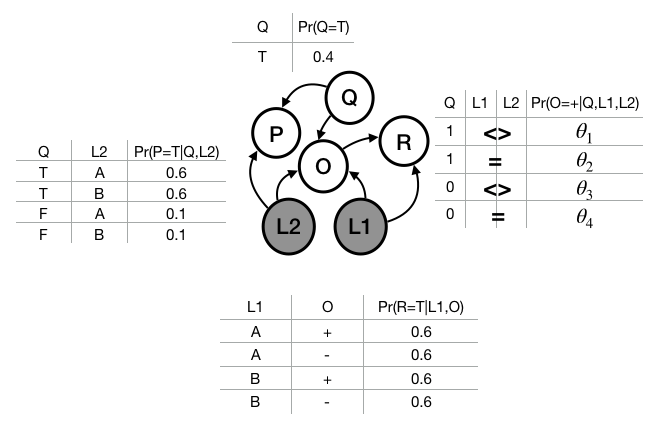
\includegraphics[width=\textwidth]{figs/BN.png}
  \end{minipage}\hfill
  \begin{minipage}[c]{0.45\textwidth}
    \caption{
        \small The model used for generating the datasets. There are four binary random variables, P, Q, O, and R. \textbf{P}: indicates whether or not the employee has high performance; \textbf{Q}: indicates whether or not an employee has high qualification; \textbf{O}: indicates whether or not the colleague submits the positive opinion towards the employee;  \textbf{R}: indicates whether or not the colleague has a positive opinion towards the employee;  \textbf{L1, L2}: indicates the label of the review provider and review receiver (observed).
    } \label{fig:BN}
  \end{minipage}
\end{figure}

We show the effectiveness of FairPSL by performing an empirical evaluation. We investigate two research questions in our experiments:
\begin{description}
\item[Q1] What is the effect of the fairness threshold $\delta$ on the fairness measures $RD/RC/RR$?
\item[Q2] How is decision quality affected by imposing $\delta$-fairness constraints?
\end{description}

Note that although we present the result for specific parameters of the framework in this section, we ran extensive analysis and the results we present are representative. We implemented the MAP inference routines of PSL and FairPSL in Python, using Gurobi-8.1\footnote{\url{www.gurobi.com}} as the backend solver. The FairPSL code, code for the data generator and data is publicly available\footnote{https://github.com/gfarnadi/FairPSL}. 

\subsection{Data generation}
  
We evaluate the FairPSL inference algorithm on synthetic datasets representing the performance review scenario (introduced in Example~\ref{ex:review}). The organization hierarchy is generated synthetically. 
The organization hierarchy generator is parameterized by two numbers: the number of employees in the organization ($n$) and the number of employees managed by each manager ($k$). Each employee is randomly assigned with a label \emph{A} or \emph{B}. An examples organization hierarchy with $n$=50 and $k$=3 is shown in Figure~\ref{fig:hierachy}.

\begin{figure}
  \begin{minipage}[c]{0.3\textwidth}
    \caption{
        \small An example of an organizational hierarchy with five levels and 50 employees with k=3. Each employee either has label A (shown with grey) or B (shown with white).
    }\label{fig:hierachy} 
	\end{minipage} \hfill
    \begin{minipage}[c]{0.7\textwidth}
    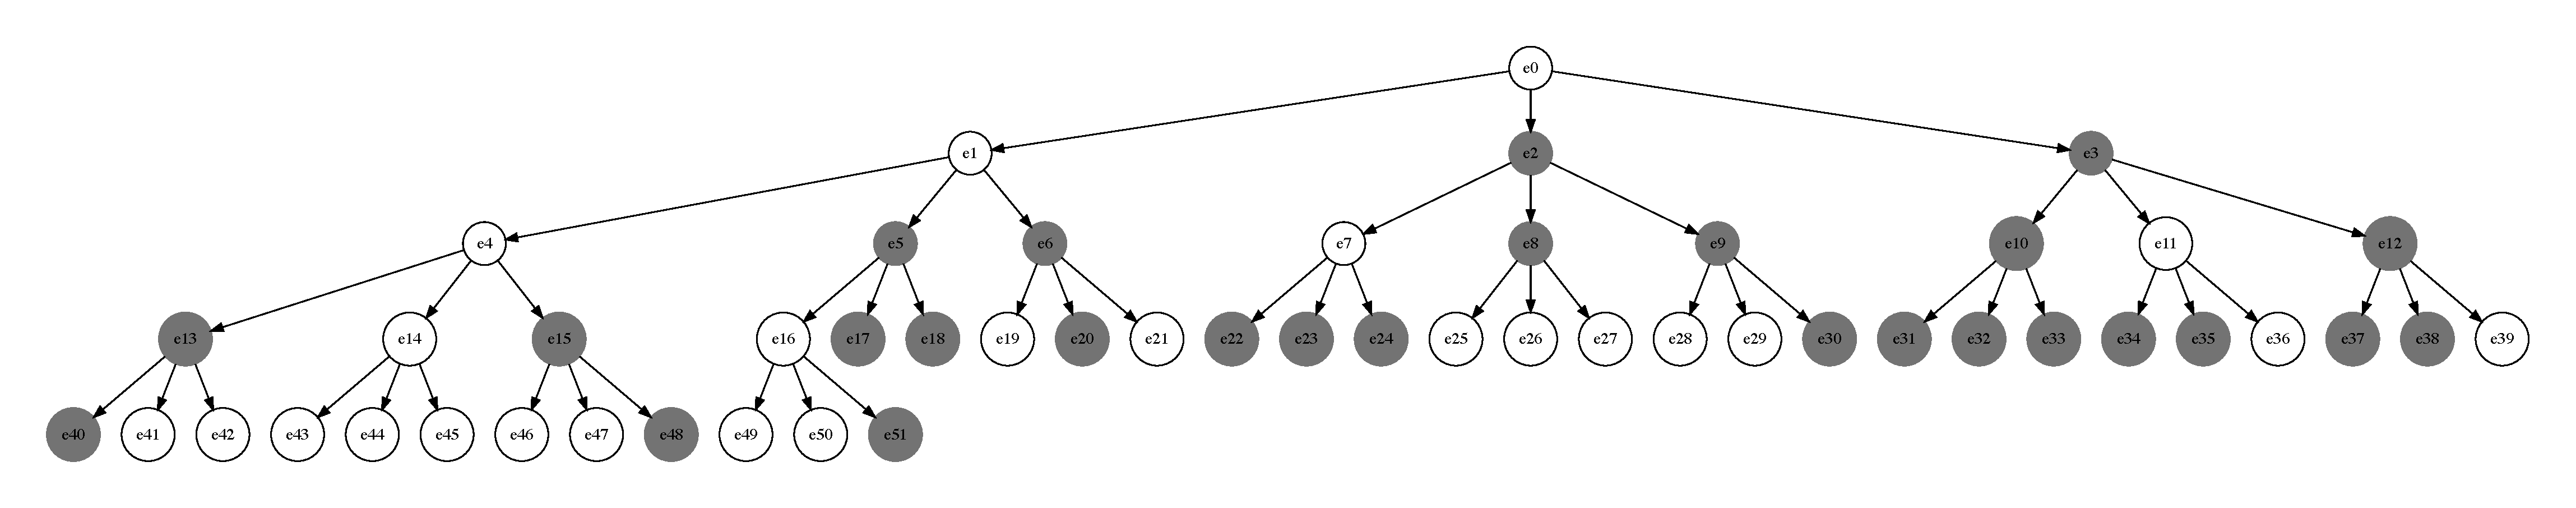
\includegraphics[width=\textwidth]{figs/Uni-hierachy.pdf}
  \end{minipage}
\end{figure}

For each employee, we use the generative model of Figure~\ref{fig:BN} to draw assignments for all the random variables. We assume that only $40\%$ of employees are qualified for promotion and regardless of their labels, employees submit only $60\%$ of their opinions. In addition, due to various personal and environmental factors, only $60\%$ of high quality employees perform well while $10\%$ of low quality employees also perform well regardless of their labels. Note that these numbers are not specific and just chosen for the framework to serve as a representative setting and a proof of concept. The conditional probability table for the opinion variable $O$ is parameterized by four values $(\theta_1, \theta_2, \theta_3, \theta_4)$ which together determine the degree of discrimination against the protected group. Since other parameters in the Bayesian network did not have a direct effect on the degree of discrimination, we fixed them to arbitrary values. 

The results presented in this section are based on an organization hierarchy  with $100$ employees where $k=5$. However, the results of the framework are not sensitive to the settings as we test the framework with various organization sizes ranging from $50$ to $500$ employees and various degree for $k$ ranging from $3$ to $10$. We generated seven datasets given the organization hierarchy using different values for the $\theta$ parameters: $(0.0,1.0,0.0,0.0)$, $(0.33,1.0,0.0,0.0)$, $(0.66,1.0,0.0,0.0)$, $(1.0,1.0,0.0,0.0)$, $(1.0,1.0,0.0,0.33)$, $(1.0,1.0,0.0,0.66)$, $(1.0,1.0,0.0,1.0)$. 
 
In the first three settings the discrimination originates from negative opinions towards qualified outgroup employees. The first setup is an extreme case where the opinion towards outgroup employees is always negative. The discrimination in the last three settings originates from positive opinions towards unqualified ingroup employees. The last setup is an extreme case where the opinion towards ingroup employees is always positive. The fourth setup represent unbiased opinions where employees are treated similarly based on their qualification. 

\paragraph{MAP Inference} We use the model presented in Table~\ref{tab:pslmodel} for MAP inference in PSL and FairPSL (recall that in FairPSL, the $\delta$-fairness constraints corresponding to one of the fairness measures are also added to the model). The observed atoms are $\textit{Manager(m,e)}$, $\textit{PositiveReview(e1,e2)}$ and labels of all employees. The truth values for all other atoms are obtained via MAP inference. We use the truth values obtained for the decision atoms $\textit{ToPromote(e)}$ to compute the fairness measures. We defined the discriminative pattern, and the protected and unprotected groups of this problem in Section~\ref{sec:formulation}.


\subsection{Evaluation results}

\begin{figure}
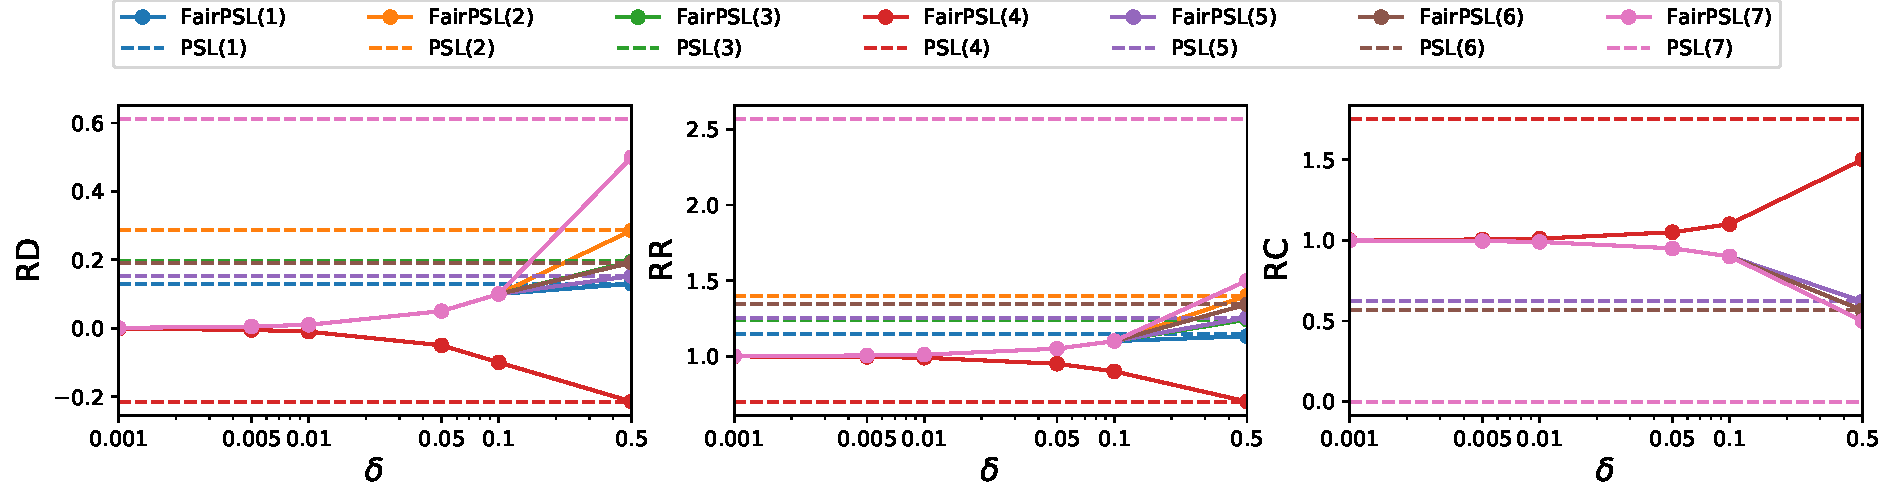
\includegraphics[width=1\linewidth]{figs/results_vis_uni_params.pdf}
\caption{\small Fairness score of predictions obtained by MAP inference of PSL and FairPSL, according to the fairness measures \emph{RD}, \emph{RR}, and \emph{RC}. The labels of datasets are mentioned with parenthesis next to the inference method. The FairPSL values of each measure are obtained by adding the $\delta$-fairness constraint of that measure.\label{fig:results}
}  
\end{figure}

To answer \textbf{Q1}, we run the MAP inference algorithm of PSL and FairPSL on seven synthetic datasets. 
We run the MAP inference of FairPSL multiple times on each dataset: For each of the three fairness measures, we add the corresponding $\delta$-fairness constraint with five thresholds $\{0.001, 0.005, 0.01, 0.05, 0.1, 0.5\}$.

Figure~\ref{fig:results} shows the fairness score of predictions in terms of the three fairness measures. As expected, tighter $\delta$-fairness constraints lead to better scores. Note that the best possible score according to RD is 0, as it computes a difference. Since RR and RC compute ratios, the best possible score according to these measures is 1. In our experiments, with any of these measures, taking $\delta = 0.001$ pushes the score of predictions to its limit.  

The $\delta$-fairness constraints modify the optimization problem of MAP inference by reducing the feasible region to solutions that conform with fairness guarantees. Research question \textbf{Q2} is concerned with the effect of this reduction on the accuracy of predictions. Note that decision quality is the same as the accuracy of predictions. To answer this question, we compare the inferred values for the decision atoms \textit{ToPromote(e)} against their actual values. These values are extracted from the known values of \textit{IsQualified(e)} according to rules 11 and 12 in Table~\ref{tab:pslmodel}. Figure~\ref{fig:accuracy} shows the area under the curve of the receiver operating characteristic~(AUC) of predicting the decision variable in three groups, namely the protected group, the unprotected group (i.e., promotion of the employees who have in-group managers), and all employees. By doing so, we make sure that our fairness constraints do not propagate bias towards either of the populations. Since the results of FairPSL with $\delta$-fairness constraints RR and RC are very similar to the results of RD, we only report the latter here.


\begin{figure}
    \centering
    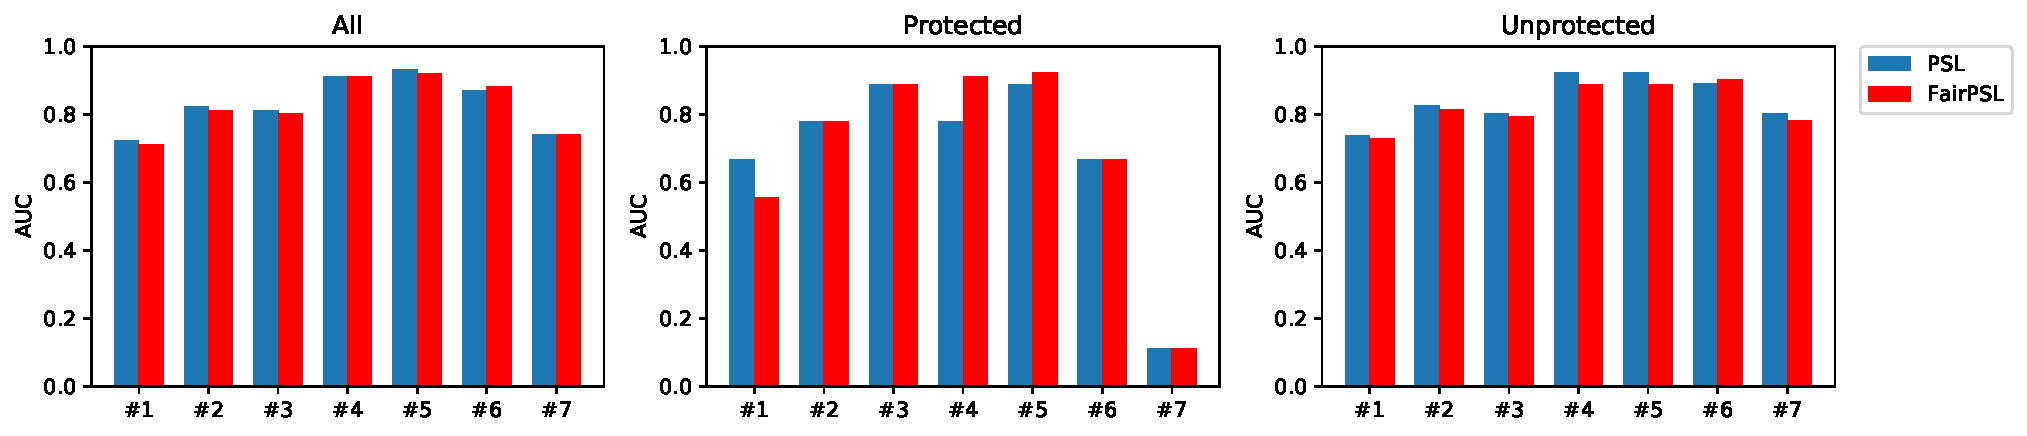
\includegraphics[width=\textwidth]{figs/roc.pdf}
    \caption{\small AUC score of predictions for truth values of unknown atoms \textit{ToPromote(e)} using MAP inference of PSL and FairPSL with $\delta$-fairness constraints $RD$ with $\delta=0.001$.}
    \label{fig:accuracy}
\end{figure}

According to Figure~\ref{fig:accuracy}, the results of both PSL and FairPSL in all seven datasets are close to each other. Note that although fairness may impose a cost in terms of overall accuracy, FairPSL often improves the accuracy of the protected class. Sometimes the overall predictions of FairPSL are even slightly better than PSL (e.g., dataset 6 and 7). As expected, the accuracy of the fourth setting where the opinions are unbiased are similar in both PSL and FairPSL. We observe that prediction of MAP inference for both FairPSL and PSL are similar, thus, in these settings at least, FairPSL guarantees fairness without hurting accuracy. Further investigation is required on the effect of the various ranges of discrimination (i.e., $\theta_1$, $\theta_2$, $\theta_3$, $\theta_4$) on the prediction results of FairPSL.



We also generate various types of organizations in which labels are not uniformly distributed, e.g., one population only occurs at the bottom levels of an organization. While we did not observe any differences in the behavior of our method with respect to accuracy and fairness measure, we found that the degree of discrimination is higher in such organizations. Further investigations on the structure of an organization on discrimination is an interesting direction for future research. 

\section{Conclusion and Future Directions}
\label{sec:conclusion}
Many applications of AI and machine learning affect peoples' lives in important ways. While there is a growing body of work on fairness in AI and ML, it assumes an individualistic notion of fairness.   In this paper, we have proposed a general framework for relational fairness which includes both a rich language for defining discrimination patterns and an efficient algorithm for performing inference subject to fairness constraints. We show our approach enforces fairness guarantees while preserving the accuracy of the predictions. 

There are many avenues for expanding on this work. For example, here we assumed that the discriminative pattern is given, however an automatic mechanism to extract discriminatory situations hidden in a large amount of decision records is an important and required task. Discrimination discovery has been studied for attribute-based fairness~\cite{pedreschi2013discovery}. An interesting next step is discrimination pattern discovery in relational data.

\section*{Acknowledgements}
This work is supported by the National Science Foundation under Grant Numbers CCF-1740850 and IIS-1703331. Golnoosh Farnadi and Behrouz Babaki are  supported by postdoctoral scholarships from IVADO through the Canada First Research Excellence Fund (CFREF) grant.

\begin{thebibliography}{10}
\itemsep=1pt 
\begin{small}

\bibitem{EUlaw}
European union legislation. (a) racial equality directive, 2000; (b) employment
  equality directive, 2000; (c) gender employment directive, 2006; (d) equal
  treatment directive (proposal), 2008.

\bibitem{UKlaw}
{UK} legislation. (a) sex discrimination act, 1975, (b) race relation act,
  1976.

\bibitem{USlaw}
United nations legislation. (a) universal declaration of human rights, 1948,
  (c) convention on the elimination of all forms of racial discrimination,
  1966, (d) convention on the elimination of all forms of discrimination
  against women, 1979.

\bibitem{alshukaili:iswc16}
Duhai Alshukaili, Alvaro A.~A. Fernandes, and Norman~W. Paton.
\newblock Structuring linked data search results using probabilistic soft
  logic.
\newblock In {\em International Semantic Web Conference {(1)}}, volume 9981 of
  {\em Lecture Notes in Computer Science}, pages 3--19, 2016.

\bibitem{bach:jmlr17}
Stephen~H. Bach, Matthias Broecheler, Bert Huang, and Lise Getoor.
\newblock Hinge-loss markov random fields and probabilistic soft logic.
\newblock {\em Journal of Machine Learning Research}, 18:109:1--109:67, 2017.

\bibitem{barocas2016big2}
Solon Barocas and Andrew~D Selbst.
\newblock Big data's disparate impact.
\newblock {\em California Law Review}, 104:671, 2016.

\bibitem{boyd2014networked}
Danah Boyd, Karen Levy, and Alice Marwick.
\newblock The networked nature of algorithmic discrimination.
\newblock In {\em Data and discrimination: Collected essays}, pages 53--57.
  2014.

\bibitem{brewer1979group}
Marilynn~B Brewer.
\newblock In-group bias in the minimal intergroup situation: A
  cognitive-motivational analysis.
\newblock {\em Psychological bulletin}, 86(2):307, 1979.

\bibitem{brewer2007social}
Marilynn~B Brewer.
\newblock The social psychology of intergroup relations: Social categorization,
  ingroup bias, and outgroup prejudice.
\newblock {\em Social Psychology: Handbook of Basic Principles}, 2007.

\bibitem{chouldechova2017fair2}
Alexandra Chouldechova.
\newblock Fair prediction with disparate impact: {A} study of bias in
  recidivism prediction instruments.
\newblock {\em CoRR}, abs/1703.00056, 2017.

\bibitem{dwork2012fairness3}
Cynthia Dwork, Moritz Hardt, Toniann Pitassi, Omer Reingold, and Richard~S.
  Zemel.
\newblock Fairness through awareness.
\newblock In {\em {ITCS}}, pages 214--226. {ACM}, 2012.

\bibitem{ebrahimi:emnlp16}
Javid Ebrahimi, Dejing Dou, and Daniel Lowd.
\newblock Weakly supervised tweet stance classification by relational
  bootstrapping.
\newblock In {\em {EMNLP}}, pages 1012--1017. The Association for Computational
  Linguistics, 2016.

\bibitem{farnadi2018fairness}
Golnoosh Farnadi, Behrouz Babaki, and Lise Getoor.
\newblock Fairness in relational domains.
\newblock In {\em AAAI/ACM Conference on AI, Ethics, and Society (AIES)}, pages
  108--114. ACM, 2018.

\bibitem{feldman2015certifying2}
Michael Feldman, Sorelle~A. Friedler, John Moeller, Carlos Scheidegger, and
  Suresh Venkatasubramanian.
\newblock Certifying and removing disparate impact.
\newblock In {\em {KDD}}, pages 259--268. {ACM}, 2015.

\bibitem{getoor2007introduction}
Lise Getoor and Ben Taskar.
\newblock {\em {Introduction to Statistical Relational Learning}}.
\newblock MIT press Cambridge, 2007.

\bibitem{hardt2016equality3}
Moritz Hardt, Eric Price, and Nati Srebro.
\newblock Equality of opportunity in supervised learning.
\newblock In {\em {NIPS}}, pages 3315--3323, 2016.

\bibitem{kamishima2011fairness}
Toshihiro Kamishima, Shotaro Akaho, and Jun Sakuma.
\newblock Fairness-aware learning through regularization approach.
\newblock In {\em ICDMW}, pages 643--650. {IEEE} Computer Society, 2011.

\bibitem{kouki:recsys15}
Pigi Kouki, Shobeir Fakhraei, James~R. Foulds, Magdalini Eirinaki, and Lise
  Getoor.
\newblock Hyper: {A} flexible and extensible probabilistic framework for hybrid
  recommender systems.
\newblock In {\em RecSys}, pages 99--106. {ACM}, 2015.

\bibitem{counterfactualfairness}
Matt~J. Kusner, Joshua~R. Loftus, Chris Russell, and Ricardo Silva.
\newblock Counterfactual fairness.
\newblock In {\em {NIPS}}, pages 4069--4079, 2017.

\bibitem{Pedreschi:2012}
Dino Pedreschi, Salvatore Ruggieri, and Franco Turini.
\newblock A study of top-k measures for discrimination discovery.
\newblock In {\em {SAC}}, pages 126--131. {ACM}, 2012.

\bibitem{pedreschi2013discovery}
Dino Pedreschi, Salvatore Ruggieri, and Franco Turini.
\newblock The discovery of discrimination.
\newblock In {\em Discrimination and Privacy in the Information Society},
  volume~3 of {\em Studies in Applied Philosophy, Epistemology and Rational
  Ethics}, pages 91--108. Springer, 2013.

\bibitem{ridgeway2004unpacking}
Cecilia~L Ridgeway and Shelley~J Correll.
\newblock Unpacking the gender system: A theoretical perspective on gender
  beliefs and social relations.
\newblock {\em Gender \& society}, 18(4):510--531, 2004.

\bibitem{sridhar:bioinformatics16}
Dhanya Sridhar, Shobeir Fakhraei, and Lise Getoor.
\newblock A probabilistic approach for collective similarity-based drug-drug
  interaction prediction.
\newblock {\em Bioinformatics}, 32(20):3175--3182, 2016.

\bibitem{verma2018fairness2}
Sahil Verma and Julia Rubin.
\newblock Fairness definitions explained.
\newblock In {\em 2018 IEEE/ACM International Workshop on Software Fairness
  (FairWare)}, pages 1--7. IEEE, 2018.

\bibitem{west2014exploiting}
Robert West, Hristo~S. Paskov, Jure Leskovec, and Christopher Potts.
\newblock Exploiting social network structure for person-to-person sentiment
  analysis.
\newblock {\em {TACL}}, 2:297--310, 2014.

\bibitem{zafar2017parity}
Muhammad~Bilal Zafar, Isabel Valera, Manuel Gomez{-}Rodriguez, Krishna~P.
  Gummadi, and Adrian Weller.
\newblock From parity to preference-based notions of fairness in
  classification.
\newblock In {\em {NIPS}}, pages 228--238, 2017.

\bibitem{zemel2013learning}
Richard~S. Zemel, Yu~Wu, Kevin Swersky, Toniann Pitassi, and Cynthia Dwork.
\newblock Learning fair representations.
\newblock In {\em {ICML} {(3)}}, volume~28 of {\em {JMLR} Workshop and
  Conference Proceedings}, pages 325--333. JMLR.org, 2013.

\end{small}
\end{thebibliography}

\end{document}

\end{article}


\begin{article}
{Platform Design for Crowdsourcing and Future of Work}
{David Gross-Amblard, Atsuyuki Morishima, Saravanan Thirumuruganathan,Marion Tommasi, Ko Yoshida}
\graphicspath{{submissions/atsuyuki/}}
%\documentclass[11pt,dvipdfm]{article}
\documentclass[11pt]{article}
\usepackage{deauthor,times,graphicx} %required
\usepackage{amsmath,amssymb}
\usepackage{multirow}
\usepackage{algorithm}
\usepackage{algpseudocode}
\usepackage{todonotes}
\usepackage{url}

% \graphicspath{{farnadi/}}

\newtheorem{mydef}{\textbf{Definition}}
\newtheorem{myex}{\textbf{Example}}
\newtheorem{mytheorem}{\textbf{Theorem}}


\begin{document}

\title{A Declarative Approach to Fairness in Relational Domains}
\author{Golnoosh Farnadi$^{1,2}$, Behrouz Babaki$^1$, Lise Getoor$^3$\\
$^1$Polytechnique Montr\'{e}al, $^2$ Mila, $^3$ UC Santa Cruz \\
farnadig@mila.quebec, behrouz.babaki@polymtl.ca, getoor@soe.ucsc.edu}

\maketitle

\begin{abstract}
AI and machine learning tools are being used with increasing frequency for decision making in domains that affect peoples' lives such as employment, education, policing and %loan approval
financial qualifications. These uses raise concerns about biases of algorithmic discrimination and have motivated the development of fairness-aware machine learning. However, existing fairness approaches are based solely on attributes of individuals. In many cases, discrimination is much more complex, and taking into account the social, organizational, and other connections between individuals is important. We introduce new notions of fairness that are able to capture the relational structure in a domain. We use first-order logic to provide a flexible and expressive language for specifying complex relational patterns of discrimination. Furthermore, we extend an existing statistical relational learning framework, probabilistic soft logic~(PSL), to incorporate our definition of relational fairness. We refer to this fairness-aware framework FairPSL. FairPSL makes use of the logical definitions of fairnesss but also supports a probabilistic interpretation. In particular, we show how to perform maximum a posteriori~(MAP) inference by exploiting probabilistic dependencies within the domain while avoiding violations of fairness guarantees. Preliminary empirical evaluation shows that we are able to make both accurate and fair decisions.
\end{abstract}

\section{Introduction}
\label{sec:introduction}

Over the past few years, AI and machine learning have become essential components in operations that drive the modern society, e.g., in financial, administrative, and educational spheres. \emph{Discrimination} happens when qualities of individuals which are not relevant to the decision making process influence the decision. Delegating decision making to an automated process raises questions about discriminating against individuals with certain traits based on biases in the data. This is especially important when the decisions have the potential to impact the lives of individuals, for example, the decisions on granting loans, assigning credit, and employment. 

\emph{Fairness} is defined as the absence of discrimination in a decision making process. The goal of \emph{fairness-aware} machine learning is to ensure that the decisions made by an algorithm do not discriminate against a population of individuals~\cite{feldman2015certifying2,boyd2014networked,hardt2016equality3}. Fairness has been well studied in the social sciences and legal scholarship (for an in-depth review see~\cite{barocas2016big2}), and there is emerging work on fairness-aware ML within the AI and computer science communities. For example, fairness through awareness/Lipschitz property~\cite{dwork2012fairness3}, individual fairness~\cite{zemel2013learning}, statistical parity/group fairness~\cite{kamishima2011fairness}, counterfactual fairness~\cite{counterfactualfairness}, demographic parity/disparate impact~\cite{feldman2015certifying2,chouldechova2017fair2}, preference-based fairness~\cite{zafar2017parity}, and equality of opportunity~\cite{hardt2016equality3}.

The existing work in fairness-aware machine learning is based on a definition of discrimination where a decision is influenced by an \emph{attribute} of an individual. An attribute value upon which discrimination is based (such as gender, race, or religion) is called a \emph{sensitive attribute}. The sensitive attribute defines a population of vulnerable individuals known as the \emph{protected group}. A fair decision-making process treats the protected group the same as the \emph{unprotected group}. 

However, in many social contexts, discrimination is the result of complex interactions and can not be described solely in terms of attributes of an individual. For example, consider an imaginary scenario in an organization in which younger female workers who have older male supervisors have lower chances of promotion than their male counterparts.\footnote{Of course, many other patterns may be possible: female bosses may promote female subordinates and discriminate against male workers, or male bosses may promote female employees.  Our goal is to provide a general framework which is able to describe arbitrarily complex discrimination patterns.} 
 This discrimination pattern involves two attributes of the individual (gender and age), a relationship with another individual (supervisor), and two attributes of the second individual. Addressing such complex cases poses two challenges. First, the concepts of discrimination and fairness need to be extended to capture not only attributes of individuals but also the relationships between them. Second, a process is required that ensures that fair decisions are made about individuals who are affected by such patterns. In this paper we address both of these challenges.
We use first-order logic (FOL) to extend the notion of fairness to the relational setting. FOL is an expressive representation for relational problems which is also widely used for learning in relational domains. Moreover, we extend an existing framework for statistical relational learning~\cite{getoor2007introduction} called probabilistic soft logic (PSL)\footnote{http://psl.linqs.org/}~\cite{bach:jmlr17}. PSL combines logic and probability for learning and reasoning over uncertain relational domains. One of the most common reasoning tasks in PSL is called maximum a posteriori (MAP) inference, which is performed by finding the most probable truth values for unknowns over a set of given evidence. We develop a new MAP inference algorithm which is able to maximize the a posteriori values of unknown variables \emph{subject to} fairness guarantees. An early version of this paper which this work builds upon and extends appeared in~\cite{farnadi2018fairness}.

\looseness-1
Our contributions are as follows: 1) we propose fairness-aware machine learning for the relational setting; 2) we extend PSL into a fairness-aware framework called FairPSL which can represent the logical definition of fairness; 3) we develop a new MAP inference algorithm which is able to maximize the posteriori values of unknown variables \emph{subject to} fairness guarantees; 4) we empirically evaluate our proposed framework on synthetic data. 

\section{Motivation}
\label{sec:motivation}

Discrimination in social contexts have been studied in the field of social psychology~\cite{brewer2007social,brewer1979group,ridgeway2004unpacking}. There is a large literature on various aspects of relational bias in social contexts such as \emph{in-group-out-group bias}, \emph{gender bias}, and \emph{ethnicity-based favoritism} that can result in discrimination. 
As an example, consider gender bias in the workplace that reflects stereotypically masculine criteria and male-based favoritism. Such gender bias 
typically places women in lower positions and negatively impacts their opportunities. Further, lack of women in leadership positions may affect the promotion of women and results in a glass ceiling that keeps women from rising beyond a certain level in the hierarchy. This scenario shows that considering  protected attributes such as gender is not always sufficient to detect the source of bias and avoid discrimination, one also has to consider the relational information, in this case the organization hierarchy. Note that this can be generalized to any ingroup/outgroup scenario where the sensitive attribute could be race, religion, age, marital-status, etc.

The existing work on designing fair algorithms in machine learning exclusively focuses on \emph{attribute-based fairness}, which is based on the following assumptions: First, there is an assumption that the individuals (sometimes referred to as units or entities) are independent and described by simple attribute vectors. Second, the group for which one wishes to ensure fairness (known as the \emph{protected group}) is defined on the basis of some attribute values. Finally, there is a decision that is associated with each individual, and the goal is to ensure that members of the protected group are subject to a fair decision (we discuss different fairness measures in Section~\ref{sec:fairnessmeasure}).  We illustrate  attribute-based fairness in the following example. 

\begin{myex}[Loan Processing]
\label{ex:loan}
A bank bases its decisions about granting a loan on attributes of the applicant. The goal is to decide whether to grant a loan to an applicant using a predictive model. The bank needs to ensure that the obey fair lending practices and ensure that gender, race, sexual orientation of applicants has no influence on the decision. In this scenario, the protected group is the historically disadvantaged applicants.  
\end{myex}
The current fairness-aware machine learning techniques are not capable of modeling relations and hence cannot be used to make the decision making model fair. However, in many decision making scenarios, especially in social and organizational settings, the domain is relational, and the protected group itself might be best represented using a relational definition. We illustrate this setting in the following scenario:
\begin{myex}[Performance Review]
\label{ex:review}
Consider an organization where decisions about the promotion of employees is based on two criteria: 1) an objective performance measure, and 2) the opinion of their direct and indirect managers above them. The opinions are inferred from the performance reviews which are collected periodically. Not every manager can submit a review for all its subordinates, this is especially the case for top-level managers who have a large number of subordinates. Hence, the opinions of managers are collectively inferred from the opinions of their sub-ordinates. However, some employees may be biased, and judge other employees unfavorably, by favoring employees who are similar to themselves (same gender, race, religion, etc.) over employees who are dissimilar. The organization needs to ensure that promotion of employees do not have any relational bias caused by in-group-out-group favoritism.

\end{myex}
Example~\ref{ex:review} describes a prediction problem over a database that consists of relations between employees. Such prediction tasks are best handled by techniques from the relational learning domain. To ensure fair prediction in such settings, we need to extend the notion of \emph{attribute-based fairness} to \emph{relational fairness}. Throughout this paper, we use the performance review problem as a running example for relational fairness.

\section{Fairness Formalism}
\label{sec:formulation}

A representation that can describe different types of entities and different relationships between them is called relational. In this section, we use first-order logic to define relational fairness. We employ first-order logic as an expressive representation formalism which can represent objects and complex relationships between them. We start by defining an atom:

\begin{mydef}[Atom]
An atom is an expression of the form $P(a_1, a_2, \ldots, a_n)$ where each argument $a_1, a_2,$ $\ldots,$ $a_n$ is either a constant or a variable. The finite set of all possible substitutions of a variable to a constant for a particular variable $a$ is called its \textit{domain} $D_{a}$. If all variables in $P(a_1, a_2, \ldots, a_n)$ are substituted by some constant from their respective domain, then we call the resulting atom a \textit{ground atom}. 
\end{mydef}

\begin{myex}
In our loan processing problem (Example~\ref{ex:loan}), we can represent applicants' attributes by atoms. For instance, atom $Female(v)$ indicates whether or not applicant $v$ is female. Similarly, we can represent relations with atoms. In the performance review problem in Example~\ref{ex:review} the atom $Manager(m,e)$ indicates whether or not employee $m$ is a direct or indirect manager of employee $e$.
\end{myex}

The relational setting provides the flexibility to express complex definitions with formulae.

\begin{mydef}[Formula] 
A formula is defined by induction: every atom is a formula. If $\alpha$ and $\beta$ are formulae, then $\alpha \vee \beta$, $\alpha \wedge \beta$, $\neg \alpha$, $\alpha \rightarrow \beta$ are formulae. If $x$ is a variable and $\alpha$ is a formula, then the quantified expressions of the form $\exists x$ $\alpha$ and $\forall x$ $\alpha$ are formulae.    
\end{mydef}

To characterize groups of individuals based on a formula, we define the notion of \emph{population}.

\begin{mydef}[Population]
We denote formula $F$ which has only one free variable $v$ (i.e., other variables in $F$ are quantified) by $F[v]$. The population defined by $F[v]$ is the set of substitutions of $v$ for which $F[v]$ holds.   
\end{mydef}


\begin{myex}
\label{ex:disformula}
Consider the formula $F[v] := \forall u, \, \textit{Manager}(u,v) \rightarrow \neg \textit{SameGroup}(u, v)$. The population specified by this formula is the set of individuals all of whose managers belong to a group different from theirs. 
\end{myex}

The truth value of a formula is derived from the truth value of atoms that it comprises, according to the rules of logic. Each possible assignment of truth values to ground atoms is called an \emph{interpretation}. 


\begin{mydef}[Interpretation]
An interpretation $I$ is a mapping that associates a truth value $I(P)$ to each ground atom $P$. For Boolean truth values, $I$ associates true to 1 and false to 0 truth values. For soft logic (see Definition~\ref{def:softlogic}) $I$ maps each ground atom $P$ to a truth value in interval $[0, 1]$.
\end{mydef}

In attribute-based fairness, it is assumed that there is a certain attribute of individuals, i.e, the sensitive attribute,  that we do not want to affect a decision. Gender, race, religion and marital status are examples of sensitive attributes. Discrimination has been defined in social science studies as a treatment in favor or against a group of individuals given their sensitive attribute. This group of individuals is the protected group. 

In a relational setting, both the sensitive attributes of an individual and their participation in various relations may have an undesired effect on the final decision. We characterize the protected group in a relational setting by means of a population. In practice, we are often interested in maintaining fairness for a specific population such as applicants, students, employees, etc. This population is then partitioned into the protected and unprotected groups. We define a \emph{discriminative pattern} which is a pair of formulae to capture these groups: 1) $F_1[v]$: to specify the difference between the protected and unprotected groups and 2) $F_2[v]$: to specify the population over which we want to maintain fairness. 

\begin{mydef}[Discriminative pattern]
A discriminative pattern is a pair $\textit{DP}[v]:=(F_1[v], F_2[v])$ , where $F_1[v]$ and $F_2[v]$ are formulae.
\end{mydef}

\begin{myex}
\label{ex:pattern}
The two formulae in the discrimination pattern $\textit{DP}[v]:= \big((\forall u, \,  \textit{Manager}(u,v) \rightarrow  \neg \textit{SameGroup}(u, v)),$ $\textit{Employee}(v)\big)$ specify two populations, namely all employees and those employees who belong to a group different from their managers.
\end{myex}

Given the definition of the discriminative pattern, we have a rich language to define the scope of the protected and unprotected groups in a relational setting.

\begin{mydef}[Protected group] Given an interpretation $I$, the protected group is a population of the form:
{$$PG :=\{ v : F_1[v] \wedge F_2[v]\}$$}
which is defined as the set of all instances hold for variable $v$ for which $F_1[v] \wedge F_2[v]$ is true under interpretation $I$, that is, $I(F_1[v] \wedge F_2[v]) = 1$. 
Similarly, the \emph{unprotected group} is a population of the form: 
{$$UG := \{ v : \neg F_1[v] \wedge  F_2[v]\}$$}
which is defined as the set of all instances hold for variable $v$ 
for which $I(\neg F_1[v] \wedge F_2[v]) = 1$. 
\end{mydef}

\begin{myex}
The protected group of the discrimination pattern specified in Example~\ref{ex:pattern} is {$PG := \big\{ v : \big(\forall u, \,$ $ \textit{Manager}(u, v) \rightarrow \neg \textit{SameGroup}(u, v)\big) \wedge \textit{Employee}(v) \big\}$} and the unprotected group is {$UG :=  \big\{ v:  \big(\exists u, \, \textit{Manager}(u,v) \wedge \textit{SameGroup}(u, v)\big) \wedge \textit{Employee}(v) \big\}$}. This means our protected group is the set of employees belonging to a group different from their managers,
and our unprotected group consists of other employees. 
\end{myex}

Discrimination is defined in terms of a treatment or decision that distinguishes between the protected and unprotected groups. Here we define the \emph{decision} atom.
\begin{mydef}[Decision atom] A decision atom $d(v)$ is an atom containing exactly one variable $v$ that specifies a decision affecting the protected group which is defined either by law or end-user.
\end{mydef}
\begin{myex}
The decision atom ${\textit ToPromote}(v)$ indicates whether or not $v$ receives a promotion.
\end{myex}

Note that the fairness formulation in this section is designed for the relational setting, however relational fairness subsumes the attribute-based fairness such that: a sensitive attribute is defined by an atom with one argument and $F_2[v]$ in discrimination pattern is $\textit{Applicant}(v)$. For example, discrimination pattern of our loan processing problem in Example~\ref{ex:loan} is of the form $\textit{DP} := ( \textit{Female}(v), \textit{Applicant}(v))$ that denotes female applicants as the protected group (i.e., $PG :=  \{ v: \textit{Female}(v) \}$) and male applicants as the unprotected group (i.e., $UG := \{ v: \neg \textit{Female}(v)\}$).


\section{Fairness Measures}
\label{sec:fairnessmeasure}

Over the past few years, many fairness measures have been introduced~\cite{verma2018fairness2}. An important class of these measures are \emph{group fairness} measures which quantify the inequality between different subgroups. Some of the most popular measures in this class include \emph{equal opportunity}, \emph{equalized odds}, and \emph{demographic parity}~\cite{hardt2016equality3}. In this paper we restrict our focus to the latter. In an attribute-value setting, demographic parity means that the decision should be independent of the protected attributes. Assume that binary variables $A$ and $C$ denote the decision and protected attributes, and the preferred value of $A$ is one. Demographic parity requires that:

\begin{equation*}
    P(A=1 | C=0) = P(A=1 | C=1)
\end{equation*}

We will now generalize this measure to the relational setting using the notations defined in Section~\ref{sec:formulation}. Let $a$ and $c$ denote the counts of denial (i.e., negative decisions) for protected and unprotected groups, and $n_{1}$ and $n_{2}$ denote their sizes, respectively. Given the decision atom $d(v)$, discriminative pattern $\textit{DP}(F_1[v], F_2[v])$, and interpretation $I$, these counts are computed by the following equations: 
{
\begin{flalign}
    & a \equiv \sum_{v \in D_v} I\big( \neg d(v) \wedge  F_1[v] \wedge F_2[v]) \label{eq:a}\\
    & c \equiv \sum_{v \in D_v} I\big( \neg d(v) \wedge  \neg F_1[v] \wedge  F_2[v]) \label{eq:c}\\
    & n_{1} \equiv \sum_{v \in D_v} I\big(F_1[v] \wedge F_2[v]) \label{eq:n1}\\
    & n_{2} \equiv \sum_{v \in D_v} I\big(\neg F_1[v] \wedge  F_2[v]) \label{eq:n2}
\end{flalign}}
The proportions of denying for protected and unprotected groups are $p_1 = \frac{a}{n_1}$ and $p_2 = \frac{c}{n_2}$, respectively. There are a number of data-driven measures~\cite{Pedreschi:2012} which quantify demographic disparity and can be defined in terms of $p_1$ and $p_2$:
\begin{itemize}
    \item \textbf{Risk difference}: $RD = p_1 - p_2$, also known as absolute risk reduction. 
    \item \textbf{Risk Ratio}: $RR = \frac{p_1}{p_2}$, also known as relative risk. 
    \item \textbf{Relative Chance}: $RC = \frac{1 - p_1}{1 - p_2}$ also, known as selection rate.
\end{itemize}
These measures have been used in the legal systems of European Union, UK, and US~\cite{EUlaw,UKlaw,USlaw}. Notice that RR is the ratio of the proportion of benefit denial between the protected and unprotected groups, while RC is the ratio of the proportion of benefit granted. Finally, we introduce the notion of $\delta$-fairness.

\begin{mydef}[$\delta$-fairness]
If a fairness measure for a decision making process falls within some $\delta$-window, then the process is \emph{$\delta\text{-fair}$}. Given $0 \leq \delta \leq 1$, the  $\delta$-windows for measures RD/RR/RC are defined as:
{\begin{flalign*}
	     - \delta \leq &RD \leq \delta \\
	     1- \delta \leq &RR \leq 1+ \delta\\
	     1- \delta \leq &RC \leq 1+ \delta
	\end{flalign*}}
\end{mydef}

To overcome the limitations of attribute-based fairness, we introduce a new statistical relational learning~(SRL) framework~\cite{getoor2007introduction} suitable for modelling fairness in relational domain. In the next section, we review probabilistic soft logic~(PSL). We then extend PSL with the definition of relational fairness introduced above in Section~\ref{sec:fairMAP}. Our fairness-aware framework, ``FairPSL'', is the first SRL framework that performs fair inference. 

\section{Background: Probabilistic Soft Logic}
\label{sec:psl}

In this section, we review the syntax and semantics of PSL, and in the next section we extend MAP inference in PSL with fairness constraints to define MAP inference in FairPSL.

PSL is a probabilistic programming language for defining hinge-loss Markov random fields~\cite{bach:jmlr17}. Unlike other SRL frameworks whose atoms are Boolean, atoms in PSL can take continuous values in the interval $[0,1]$. PSL is an expressive modeling language that can incorporate domain knowledge with first-order logical rules and has been used successfully in various domains, including bioinformatics~\cite{sridhar:bioinformatics16}, recommender systems~\cite{kouki:recsys15}, natural language processing~\cite{ebrahimi:emnlp16}, information retrieval~\cite{alshukaili:iswc16}, and social network analysis~\cite{west2014exploiting}, among many others. 
 
A PSL model is defined by a set of first-order logical rules called \emph{PSL rules}.

\begin{mydef} [PSL rule] a PSL rule $r$ is an expression of the form:
{\begin{equation}
\lambda_{r}: T_1 \land T_2 \land \ldots \land T_w \rightarrow H_1 \vee H_2 \vee \ldots \vee H_l
\end{equation}}

where { $T_1, T_2, \ldots, T_w, H_1, H_2, \ldots, H_l$} are atoms or negated atoms and { $\lambda_{r} \in \mathbb{R}^{+} \cup \infty$} is the weight of the rule $r$.  We call { $T_1 \land T_2 \land \ldots \land T_w$} the body of $r$ ($r_{body}$), and { $H_1 \vee H_2 \vee \ldots \vee H_l$} the head of $r$ ($r_{head}$).
\end{mydef}


Since atoms in PSL take on continuous values in the unit interval $[0,1]$, next we define soft logic to calculate the value of the PSL rules under an interpretation $I$.

\begin{mydef}[Soft logic]
\label{def:softlogic}
The ({$\tilde{\wedge}$}) and ({$\tilde{\vee}$}) and negation ({$\tilde{\neg}$}) are defined as follows. For {$m, n \in [0,1]$} we have: {$m \tilde{\wedge} n = \max(m+n -1, 0)$}, {$m \tilde{\vee} n = \min(m+n , 1)$} and {$\tilde{\neg} m = 1 - m$}. The $\, \tilde{} \,$ indicates the relaxation over Boolean values.
\end{mydef}

The probability of truth value assignments in PSL is determined by the rules' \emph{distance to satisfaction}.

\begin{mydef}[The distance to satisfaction]
The distance to satisfaction $d_{r}(I)$ of a rule $r$ under an interpretation $I$ is defined as:
{
\begin{equation}
d_{r}(I) = \max\{0, I(r_{body})-I(r_{head})\}
\end{equation}}
\end{mydef}

By using Definition~\ref{def:softlogic}, one can show that the closer the interpretation of a grounded rule $r$ is to 1, the smaller its distance to satisfaction. A PSL model induces a distribution over interpretations $I$. Let $R$ be the set of all grounded rules, then the probability density function is:
{
\begin{equation}
f(I) ={\frac{1}{Z}} \exp[-\sum_{r\in R} \lambda_{r}(d_{r}(I))^p]
\label{eq:potential}
\end{equation}
}
\noindent where { $\lambda_{r}$} is the weight of rule $r$, {
$Z = \int_{I} \exp[ -\sum_{r\in R} \lambda_{r}(d_{r}(I))^p]$
} is a normalization constant, and { $p \in \{1,2\}$} provides a choice of two different loss functions, $p=1$ (i.e., linear), and $p=2$ (i.e, quadratic). These probabilistic models are instances of hinge-loss Markov random fields~(HL-MRF)~\cite{bach:jmlr17}. The goal of maximum a posteriori (MAP) inference is to find the most probable truth assignments $I_{\textit{MPE}}$ of unknown ground atoms given the evidence which is defined by the interpretation $I$. Let $X$ be all the evidence, i.e., $X$ is the set of ground atoms such that $\forall x \in X, I(x)$ is known, and let $Y$ be the set of ground atoms such that $\forall y \in Y, I(y)$ is unknown. Then we have
{
\begin{equation}
I_{\textit{MAP}}(Y) = \textit{arg}\max_{I(Y)} P(I(Y)|I(X))
\end{equation}}
Maximizing the density function in Equation~\ref{eq:potential} is equivalent to minimizing the weighted sum of the distances to satisfaction of all rules in PSL. 

\begin{table*}[t]
    \centering
    \begin{tabular}{|lll|}
    \hline
    &&\\
    $R1$ & $\lambda_1$ &: $\textit{IsQualified}(e) \rightarrow \textit{HighPerformance}(e)$ \\
    $R2$ & $\lambda_1$ &: $\neg \textit{IsQualified}(e) \rightarrow \neg \textit{HighPerformance}(e)$ \\
    $R3$ & $\infty$ &: $\textit{PositiveReview}(e1, e2) \rightarrow \textit{PositiveOpinion}(e1, e2)$ \\
    $R4$ & $\infty$ &: $\neg \textit{PositiveReview}(e1, e2) \rightarrow \neg \textit{PositiveOpinion}(e1, e2)$ \\
    $R5$ & $\lambda_1$ &: $\textit{PositiveOpinion}(e1, e2) \wedge \textit{Manager}(m, e1) \rightarrow \textit{PositiveOpinion}(m, e2)$ \\
    $R6$ & $\lambda_1$ &: $\neg \textit{PositiveOpinion}(e1, e2) \wedge \textit{Manager}(m, e1) \rightarrow \neg \textit{PositiveOpinion}(m, e2)$ \\
    $R7$ & $\lambda_1$ &: $\textit{PositiveOpinion}(m, e) \wedge \textit{Manager}(m, e) \rightarrow \textit{IsQualified}(e)$ \\
    $R8$ & $\lambda_1$ &: $\neg \textit{PositiveOpinion}(m, e) \wedge \textit{Manager}(m, e) \rightarrow \neg \textit{IsQualified}(e)$ \\
    $R9$ &  $\lambda_1$ &: $\neg \textit{ToPromote}(e)$\\
    $R10$ & $\infty$ &: $\textit{IsQualified}(e) \rightarrow \textit{ToPromote}(e)$ \\
    $R11$ & $\infty$ &: $\neg \textit{IsQualified}(e) \rightarrow \neg \textit{ToPromote}(e)$ \\
    &&\\
    \hline
    \end{tabular}
    \caption{\small A simplified PSL model for the \emph{Performance Reviewing} problem}
    \label{tab:pslmodel}
\end{table*}

\begin{myex}
\label{ex:pslmodel}
The simplified PSL model for the performance reviewing problem in Example\ref{ex:review} is given in Table~\ref{tab:pslmodel}. The goal of MAP inference for this problem is to infer employees to promote. We simplified the model by assigning the same weight to all soft rules (i.e., $\lambda_i= 1$ where $i=\{1,2,5,6,7,8,9\}$). Below we explain the meaning of each rule in the model.

Rule $R1$ indicates that qualified employees have high performance and similarly rule $R2$ expresses that a negative qualification of employees is derived from their low performance. Rules $R5$ and $R6$ presents the propagation of opinion from bottom to top of the organizational hierarchy, i.e., managers have similar opinions towards employees given the opinions of their sub-ordinate managers. And rules $R7$ and $R8$ indicate that the positive/negative opinion of direct/indirect managers derive from the qualification of an employee. Rule $R9$ indicates the prior that not all employees get promoted. We also have four hard constraints (i.e., rules $R3$, $R4$, $R10$ and $R11$) where the weight of the rules are $\infty$. Rules $R3$ and $R4$ indicate that submitted positive/negative reviews should reflect positive/negative opinions. And two rules $R10$ and $R11$ show that a highly qualified employee should get promoted. 
\end{myex}

\section{Fairness-aware PSL (FairPSL)}
\label{sec:fairMAP}

The standard MAP inference in PSL aims at finding values that maximize the conditional probability of unknowns. Once a decision is made according to these values, one can use the fairness measure to quantify the degree of discrimination. A simple way to incorporate fairness in MAP inference is to add the $\delta$-fairness constraints to the corresponding optimization problem.   

Consider risk difference, $\textit{RD}$, where $\textit{RD} \equiv \frac{\mathbf{a}}{n_1} - \frac{\mathbf{c}}{n_2}$. The $\delta$-fairness constraint $-\delta \leq \textit{RD} \leq \delta$ can be encoded as the following constraints:
{\begin{align}
    & n_2 \mathbf{a} - n_1 \mathbf{c} - n_1 n_2 \delta \leq 0 \label{eq:RD1}\\
    & n_2 \mathbf{a} - n_1 \mathbf{c} + n_1 n_2 \delta \geq 0
\end{align}}
Similarly, from $\textit{RR} \equiv \frac{\mathbf{a} / n_1}{\mathbf{c} / n_2}$ and the $\delta$-fairness constraint $1 - \delta \leq \textit{RR} \leq 1 + \delta$ we obtain:
{\begin{align}
    & n_2 \mathbf{a} - (1 + \delta) n_1 \mathbf{c} \leq 0 \\
    & n_2 \mathbf{a} - (1 - \delta) n_1 \mathbf{c} \geq 0
\end{align}}
And finally, $\textit{RC} \equiv \frac{1 - \mathbf{a} / n_1}{1 - \mathbf{c} / n_2}$ and the $\delta$-fairness constraint $1 - \delta \leq \textit{RC} \leq 1 + \delta$ gives:
{ \begin{align}
    & - n_2 \mathbf{a} + (1 + \delta) n_1 \mathbf{c} - \delta n_1 n_2 \leq 0 \\
    & - n_2 \mathbf{a} + (1 - \delta) n_1 \mathbf{c} + \delta n_1 n_2 \geq 0 \label{eq:RC2}
\end{align}}
A primary advantage of PSL over similar frameworks is that its MAP inference task reduces to a convex optimization problem which can be solved in polynomial time. To preserve this advantage, we need to ensure that the problem will remain convex after the addition of $\delta$-fairness constraints. 

\begin{mytheorem}
The following condition is sufficient for preserving the convexity of MAP inference problem after addition of $\delta$-fairness constraints: The formulae $F_1[v]$ and $F_2[v]$ do not contain an atom $y \in Y$ and all atoms in $F_1[v]$ and $F_2[v]$ have values zero or one.
\end{mytheorem}
\begin{proof}
Since $I(F_1[v])$ and $I(F_2[v])$ do not depend on $I(Y)$, the values $n_{1}$ and $n_{2}$ are constants that can be computed in advance. Let us define the sets $D_v^a = \{ v \in D_v : F_1[v] \wedge F_2[v] \, \text{is true} \}$ and $D_v^c = \{ v \in D_v : \neg F_1[v] \wedge F_2[v] \, \text{is true} \}$. Since $F_1[v]$ and $F_2[v]$ can be only zero or one, we can rewrite the equations~\ref{eq:a} and \ref{eq:c} as:
{
\begin{align*}
    & \mathbf{a} = \sum_{v \in D_v^a} I(\neg d(v)) = |D_v^a| - \sum_{v \in D_v^a} I(d(v))\\
    & \mathbf{c} = \sum_{v \in D_v^c} I(\neg d(v)) = |D_v^c| - \sum_{v \in D_v^c} I(d(v))
\end{align*}}
\noindent which indicates that $\mathbf{a}$ and $\mathbf{c}$ can be expressed as linear combinations of variables in the optimization problem. This means that constraints~\ref{eq:RD1}-\ref{eq:RC2} are linear. Hence, addition of these constraints preserves the convexity of the optimization problem. 
\end{proof}

\section{Experiments}
\label{sec:experiment}

\begin{figure}
  \begin{minipage}[c]{0.6\textwidth}
    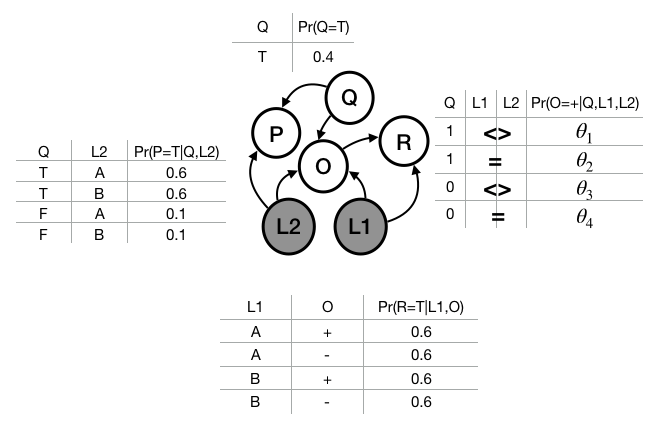
\includegraphics[width=\textwidth]{figs/BN.png}
  \end{minipage}\hfill
  \begin{minipage}[c]{0.45\textwidth}
    \caption{
        \small The model used for generating the datasets. There are four binary random variables, P, Q, O, and R. \textbf{P}: indicates whether or not the employee has high performance; \textbf{Q}: indicates whether or not an employee has high qualification; \textbf{O}: indicates whether or not the colleague submits the positive opinion towards the employee;  \textbf{R}: indicates whether or not the colleague has a positive opinion towards the employee;  \textbf{L1, L2}: indicates the label of the review provider and review receiver (observed).
    } \label{fig:BN}
  \end{minipage}
\end{figure}

We show the effectiveness of FairPSL by performing an empirical evaluation. We investigate two research questions in our experiments:
\begin{description}
\item[Q1] What is the effect of the fairness threshold $\delta$ on the fairness measures $RD/RC/RR$?
\item[Q2] How is decision quality affected by imposing $\delta$-fairness constraints?
\end{description}

Note that although we present the result for specific parameters of the framework in this section, we ran extensive analysis and the results we present are representative. We implemented the MAP inference routines of PSL and FairPSL in Python, using Gurobi-8.1\footnote{\url{www.gurobi.com}} as the backend solver. The FairPSL code, code for the data generator and data is publicly available\footnote{https://github.com/gfarnadi/FairPSL}. 

\subsection{Data generation}
  
We evaluate the FairPSL inference algorithm on synthetic datasets representing the performance review scenario (introduced in Example~\ref{ex:review}). The organization hierarchy is generated synthetically. 
The organization hierarchy generator is parameterized by two numbers: the number of employees in the organization ($n$) and the number of employees managed by each manager ($k$). Each employee is randomly assigned with a label \emph{A} or \emph{B}. An examples organization hierarchy with $n$=50 and $k$=3 is shown in Figure~\ref{fig:hierachy}.

\begin{figure}
  \begin{minipage}[c]{0.3\textwidth}
    \caption{
        \small An example of an organizational hierarchy with five levels and 50 employees with k=3. Each employee either has label A (shown with grey) or B (shown with white).
    }\label{fig:hierachy} 
	\end{minipage} \hfill
    \begin{minipage}[c]{0.7\textwidth}
    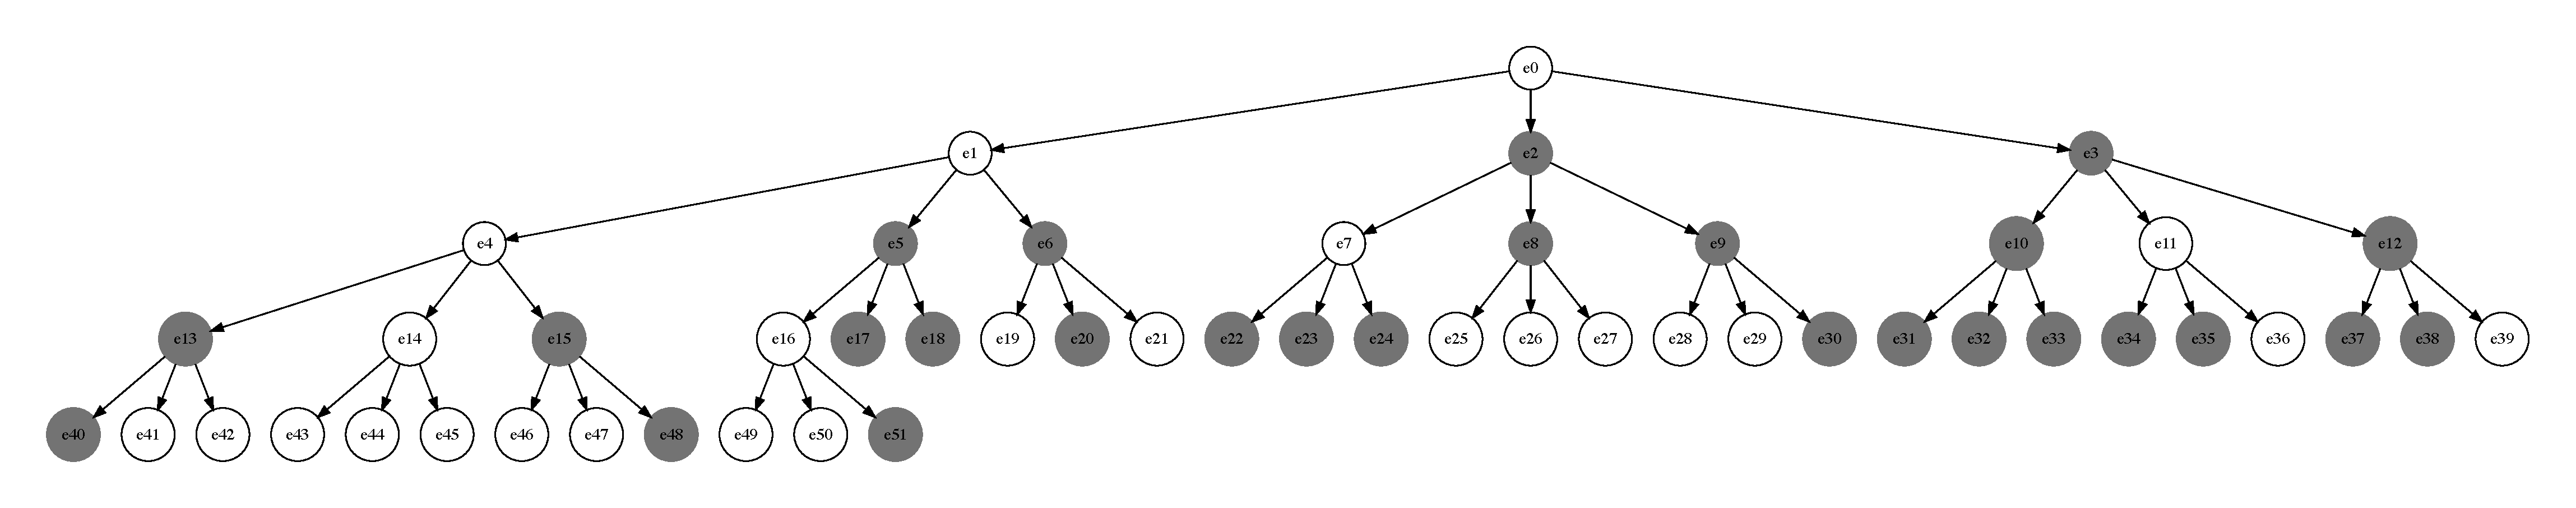
\includegraphics[width=\textwidth]{figs/Uni-hierachy.pdf}
  \end{minipage}
\end{figure}

For each employee, we use the generative model of Figure~\ref{fig:BN} to draw assignments for all the random variables. We assume that only $40\%$ of employees are qualified for promotion and regardless of their labels, employees submit only $60\%$ of their opinions. In addition, due to various personal and environmental factors, only $60\%$ of high quality employees perform well while $10\%$ of low quality employees also perform well regardless of their labels. Note that these numbers are not specific and just chosen for the framework to serve as a representative setting and a proof of concept. The conditional probability table for the opinion variable $O$ is parameterized by four values $(\theta_1, \theta_2, \theta_3, \theta_4)$ which together determine the degree of discrimination against the protected group. Since other parameters in the Bayesian network did not have a direct effect on the degree of discrimination, we fixed them to arbitrary values. 

The results presented in this section are based on an organization hierarchy  with $100$ employees where $k=5$. However, the results of the framework are not sensitive to the settings as we test the framework with various organization sizes ranging from $50$ to $500$ employees and various degree for $k$ ranging from $3$ to $10$. We generated seven datasets given the organization hierarchy using different values for the $\theta$ parameters: $(0.0,1.0,0.0,0.0)$, $(0.33,1.0,0.0,0.0)$, $(0.66,1.0,0.0,0.0)$, $(1.0,1.0,0.0,0.0)$, $(1.0,1.0,0.0,0.33)$, $(1.0,1.0,0.0,0.66)$, $(1.0,1.0,0.0,1.0)$. 
 
In the first three settings the discrimination originates from negative opinions towards qualified outgroup employees. The first setup is an extreme case where the opinion towards outgroup employees is always negative. The discrimination in the last three settings originates from positive opinions towards unqualified ingroup employees. The last setup is an extreme case where the opinion towards ingroup employees is always positive. The fourth setup represent unbiased opinions where employees are treated similarly based on their qualification. 

\paragraph{MAP Inference} We use the model presented in Table~\ref{tab:pslmodel} for MAP inference in PSL and FairPSL (recall that in FairPSL, the $\delta$-fairness constraints corresponding to one of the fairness measures are also added to the model). The observed atoms are $\textit{Manager(m,e)}$, $\textit{PositiveReview(e1,e2)}$ and labels of all employees. The truth values for all other atoms are obtained via MAP inference. We use the truth values obtained for the decision atoms $\textit{ToPromote(e)}$ to compute the fairness measures. We defined the discriminative pattern, and the protected and unprotected groups of this problem in Section~\ref{sec:formulation}.


\subsection{Evaluation results}

\begin{figure}
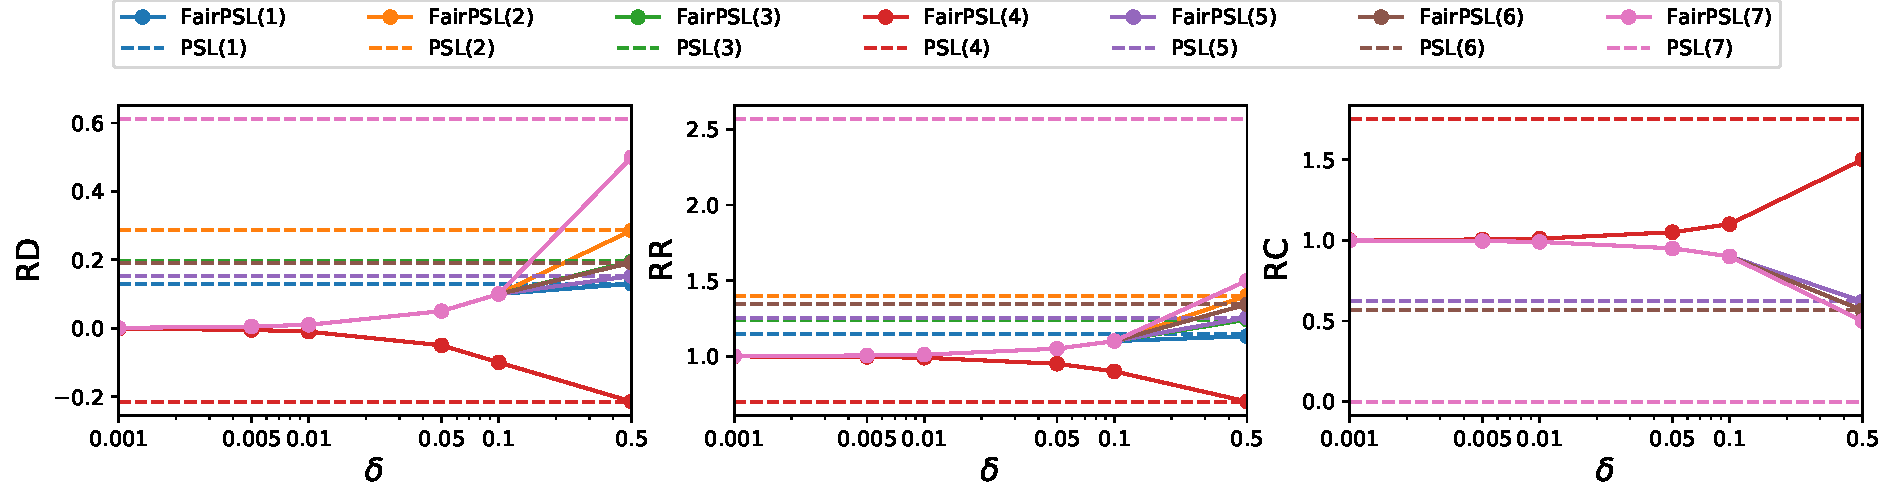
\includegraphics[width=1\linewidth]{figs/results_vis_uni_params.pdf}
\caption{\small Fairness score of predictions obtained by MAP inference of PSL and FairPSL, according to the fairness measures \emph{RD}, \emph{RR}, and \emph{RC}. The labels of datasets are mentioned with parenthesis next to the inference method. The FairPSL values of each measure are obtained by adding the $\delta$-fairness constraint of that measure.\label{fig:results}
}  
\end{figure}

To answer \textbf{Q1}, we run the MAP inference algorithm of PSL and FairPSL on seven synthetic datasets. 
We run the MAP inference of FairPSL multiple times on each dataset: For each of the three fairness measures, we add the corresponding $\delta$-fairness constraint with five thresholds $\{0.001, 0.005, 0.01, 0.05, 0.1, 0.5\}$.

Figure~\ref{fig:results} shows the fairness score of predictions in terms of the three fairness measures. As expected, tighter $\delta$-fairness constraints lead to better scores. Note that the best possible score according to RD is 0, as it computes a difference. Since RR and RC compute ratios, the best possible score according to these measures is 1. In our experiments, with any of these measures, taking $\delta = 0.001$ pushes the score of predictions to its limit.  

The $\delta$-fairness constraints modify the optimization problem of MAP inference by reducing the feasible region to solutions that conform with fairness guarantees. Research question \textbf{Q2} is concerned with the effect of this reduction on the accuracy of predictions. Note that decision quality is the same as the accuracy of predictions. To answer this question, we compare the inferred values for the decision atoms \textit{ToPromote(e)} against their actual values. These values are extracted from the known values of \textit{IsQualified(e)} according to rules 11 and 12 in Table~\ref{tab:pslmodel}. Figure~\ref{fig:accuracy} shows the area under the curve of the receiver operating characteristic~(AUC) of predicting the decision variable in three groups, namely the protected group, the unprotected group (i.e., promotion of the employees who have in-group managers), and all employees. By doing so, we make sure that our fairness constraints do not propagate bias towards either of the populations. Since the results of FairPSL with $\delta$-fairness constraints RR and RC are very similar to the results of RD, we only report the latter here.


\begin{figure}
    \centering
    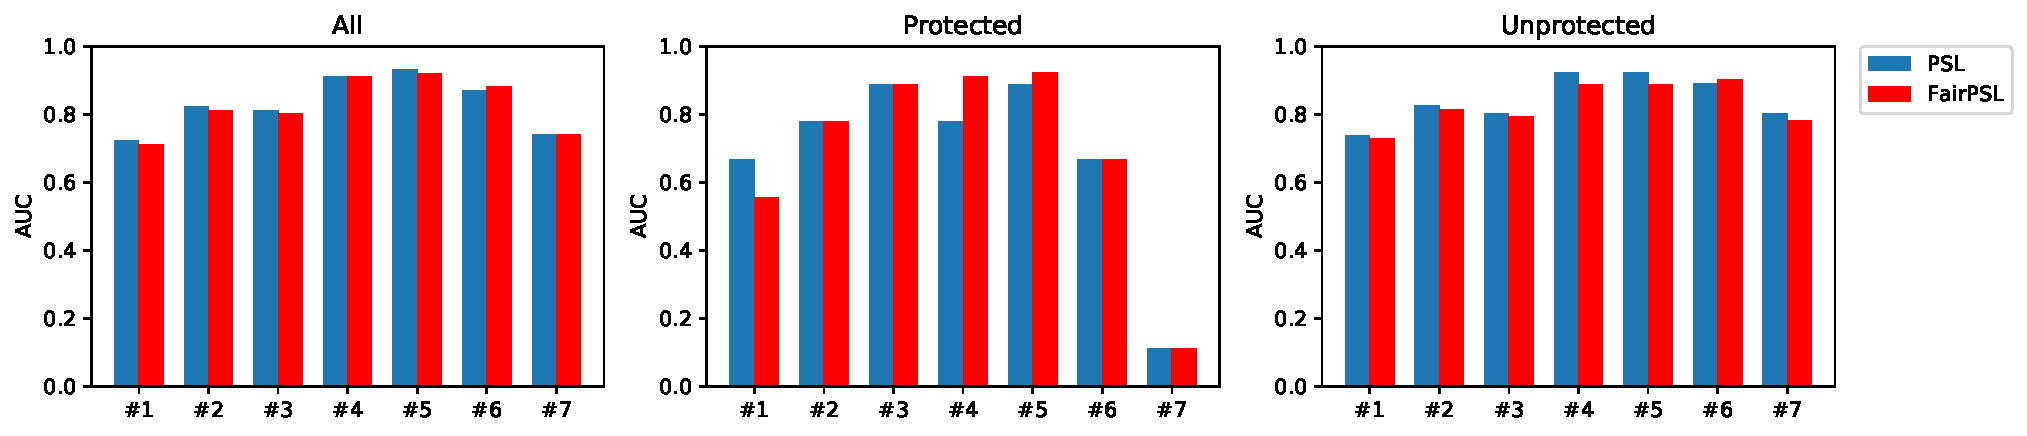
\includegraphics[width=\textwidth]{figs/roc.pdf}
    \caption{\small AUC score of predictions for truth values of unknown atoms \textit{ToPromote(e)} using MAP inference of PSL and FairPSL with $\delta$-fairness constraints $RD$ with $\delta=0.001$.}
    \label{fig:accuracy}
\end{figure}

According to Figure~\ref{fig:accuracy}, the results of both PSL and FairPSL in all seven datasets are close to each other. Note that although fairness may impose a cost in terms of overall accuracy, FairPSL often improves the accuracy of the protected class. Sometimes the overall predictions of FairPSL are even slightly better than PSL (e.g., dataset 6 and 7). As expected, the accuracy of the fourth setting where the opinions are unbiased are similar in both PSL and FairPSL. We observe that prediction of MAP inference for both FairPSL and PSL are similar, thus, in these settings at least, FairPSL guarantees fairness without hurting accuracy. Further investigation is required on the effect of the various ranges of discrimination (i.e., $\theta_1$, $\theta_2$, $\theta_3$, $\theta_4$) on the prediction results of FairPSL.



We also generate various types of organizations in which labels are not uniformly distributed, e.g., one population only occurs at the bottom levels of an organization. While we did not observe any differences in the behavior of our method with respect to accuracy and fairness measure, we found that the degree of discrimination is higher in such organizations. Further investigations on the structure of an organization on discrimination is an interesting direction for future research. 

\section{Conclusion and Future Directions}
\label{sec:conclusion}
Many applications of AI and machine learning affect peoples' lives in important ways. While there is a growing body of work on fairness in AI and ML, it assumes an individualistic notion of fairness.   In this paper, we have proposed a general framework for relational fairness which includes both a rich language for defining discrimination patterns and an efficient algorithm for performing inference subject to fairness constraints. We show our approach enforces fairness guarantees while preserving the accuracy of the predictions. 

There are many avenues for expanding on this work. For example, here we assumed that the discriminative pattern is given, however an automatic mechanism to extract discriminatory situations hidden in a large amount of decision records is an important and required task. Discrimination discovery has been studied for attribute-based fairness~\cite{pedreschi2013discovery}. An interesting next step is discrimination pattern discovery in relational data.

\section*{Acknowledgements}
This work is supported by the National Science Foundation under Grant Numbers CCF-1740850 and IIS-1703331. Golnoosh Farnadi and Behrouz Babaki are  supported by postdoctoral scholarships from IVADO through the Canada First Research Excellence Fund (CFREF) grant.

\begin{thebibliography}{10}
\itemsep=1pt 
\begin{small}

\bibitem{EUlaw}
European union legislation. (a) racial equality directive, 2000; (b) employment
  equality directive, 2000; (c) gender employment directive, 2006; (d) equal
  treatment directive (proposal), 2008.

\bibitem{UKlaw}
{UK} legislation. (a) sex discrimination act, 1975, (b) race relation act,
  1976.

\bibitem{USlaw}
United nations legislation. (a) universal declaration of human rights, 1948,
  (c) convention on the elimination of all forms of racial discrimination,
  1966, (d) convention on the elimination of all forms of discrimination
  against women, 1979.

\bibitem{alshukaili:iswc16}
Duhai Alshukaili, Alvaro A.~A. Fernandes, and Norman~W. Paton.
\newblock Structuring linked data search results using probabilistic soft
  logic.
\newblock In {\em International Semantic Web Conference {(1)}}, volume 9981 of
  {\em Lecture Notes in Computer Science}, pages 3--19, 2016.

\bibitem{bach:jmlr17}
Stephen~H. Bach, Matthias Broecheler, Bert Huang, and Lise Getoor.
\newblock Hinge-loss markov random fields and probabilistic soft logic.
\newblock {\em Journal of Machine Learning Research}, 18:109:1--109:67, 2017.

\bibitem{barocas2016big2}
Solon Barocas and Andrew~D Selbst.
\newblock Big data's disparate impact.
\newblock {\em California Law Review}, 104:671, 2016.

\bibitem{boyd2014networked}
Danah Boyd, Karen Levy, and Alice Marwick.
\newblock The networked nature of algorithmic discrimination.
\newblock In {\em Data and discrimination: Collected essays}, pages 53--57.
  2014.

\bibitem{brewer1979group}
Marilynn~B Brewer.
\newblock In-group bias in the minimal intergroup situation: A
  cognitive-motivational analysis.
\newblock {\em Psychological bulletin}, 86(2):307, 1979.

\bibitem{brewer2007social}
Marilynn~B Brewer.
\newblock The social psychology of intergroup relations: Social categorization,
  ingroup bias, and outgroup prejudice.
\newblock {\em Social Psychology: Handbook of Basic Principles}, 2007.

\bibitem{chouldechova2017fair2}
Alexandra Chouldechova.
\newblock Fair prediction with disparate impact: {A} study of bias in
  recidivism prediction instruments.
\newblock {\em CoRR}, abs/1703.00056, 2017.

\bibitem{dwork2012fairness3}
Cynthia Dwork, Moritz Hardt, Toniann Pitassi, Omer Reingold, and Richard~S.
  Zemel.
\newblock Fairness through awareness.
\newblock In {\em {ITCS}}, pages 214--226. {ACM}, 2012.

\bibitem{ebrahimi:emnlp16}
Javid Ebrahimi, Dejing Dou, and Daniel Lowd.
\newblock Weakly supervised tweet stance classification by relational
  bootstrapping.
\newblock In {\em {EMNLP}}, pages 1012--1017. The Association for Computational
  Linguistics, 2016.

\bibitem{farnadi2018fairness}
Golnoosh Farnadi, Behrouz Babaki, and Lise Getoor.
\newblock Fairness in relational domains.
\newblock In {\em AAAI/ACM Conference on AI, Ethics, and Society (AIES)}, pages
  108--114. ACM, 2018.

\bibitem{feldman2015certifying2}
Michael Feldman, Sorelle~A. Friedler, John Moeller, Carlos Scheidegger, and
  Suresh Venkatasubramanian.
\newblock Certifying and removing disparate impact.
\newblock In {\em {KDD}}, pages 259--268. {ACM}, 2015.

\bibitem{getoor2007introduction}
Lise Getoor and Ben Taskar.
\newblock {\em {Introduction to Statistical Relational Learning}}.
\newblock MIT press Cambridge, 2007.

\bibitem{hardt2016equality3}
Moritz Hardt, Eric Price, and Nati Srebro.
\newblock Equality of opportunity in supervised learning.
\newblock In {\em {NIPS}}, pages 3315--3323, 2016.

\bibitem{kamishima2011fairness}
Toshihiro Kamishima, Shotaro Akaho, and Jun Sakuma.
\newblock Fairness-aware learning through regularization approach.
\newblock In {\em ICDMW}, pages 643--650. {IEEE} Computer Society, 2011.

\bibitem{kouki:recsys15}
Pigi Kouki, Shobeir Fakhraei, James~R. Foulds, Magdalini Eirinaki, and Lise
  Getoor.
\newblock Hyper: {A} flexible and extensible probabilistic framework for hybrid
  recommender systems.
\newblock In {\em RecSys}, pages 99--106. {ACM}, 2015.

\bibitem{counterfactualfairness}
Matt~J. Kusner, Joshua~R. Loftus, Chris Russell, and Ricardo Silva.
\newblock Counterfactual fairness.
\newblock In {\em {NIPS}}, pages 4069--4079, 2017.

\bibitem{Pedreschi:2012}
Dino Pedreschi, Salvatore Ruggieri, and Franco Turini.
\newblock A study of top-k measures for discrimination discovery.
\newblock In {\em {SAC}}, pages 126--131. {ACM}, 2012.

\bibitem{pedreschi2013discovery}
Dino Pedreschi, Salvatore Ruggieri, and Franco Turini.
\newblock The discovery of discrimination.
\newblock In {\em Discrimination and Privacy in the Information Society},
  volume~3 of {\em Studies in Applied Philosophy, Epistemology and Rational
  Ethics}, pages 91--108. Springer, 2013.

\bibitem{ridgeway2004unpacking}
Cecilia~L Ridgeway and Shelley~J Correll.
\newblock Unpacking the gender system: A theoretical perspective on gender
  beliefs and social relations.
\newblock {\em Gender \& society}, 18(4):510--531, 2004.

\bibitem{sridhar:bioinformatics16}
Dhanya Sridhar, Shobeir Fakhraei, and Lise Getoor.
\newblock A probabilistic approach for collective similarity-based drug-drug
  interaction prediction.
\newblock {\em Bioinformatics}, 32(20):3175--3182, 2016.

\bibitem{verma2018fairness2}
Sahil Verma and Julia Rubin.
\newblock Fairness definitions explained.
\newblock In {\em 2018 IEEE/ACM International Workshop on Software Fairness
  (FairWare)}, pages 1--7. IEEE, 2018.

\bibitem{west2014exploiting}
Robert West, Hristo~S. Paskov, Jure Leskovec, and Christopher Potts.
\newblock Exploiting social network structure for person-to-person sentiment
  analysis.
\newblock {\em {TACL}}, 2:297--310, 2014.

\bibitem{zafar2017parity}
Muhammad~Bilal Zafar, Isabel Valera, Manuel Gomez{-}Rodriguez, Krishna~P.
  Gummadi, and Adrian Weller.
\newblock From parity to preference-based notions of fairness in
  classification.
\newblock In {\em {NIPS}}, pages 228--238, 2017.

\bibitem{zemel2013learning}
Richard~S. Zemel, Yu~Wu, Kevin Swersky, Toniann Pitassi, and Cynthia Dwork.
\newblock Learning fair representations.
\newblock In {\em {ICML} {(3)}}, volume~28 of {\em {JMLR} Workshop and
  Conference Proceedings}, pages 325--333. JMLR.org, 2013.

\end{small}
\end{thebibliography}

\end{document}

\end{article}



\begin{article}
{On Benchmarking for Crowdsourcing and Future of Work Platforms}
{Ria Mae Borromeo, Lei Chen, Abhishek Dubey, Sudeepa Roy, Saravanan Thirumuruganathan}
\graphicspath{{submissions/Learning/}}
%\documentclass[11pt,dvipdfm]{article}
\documentclass[11pt]{article}
\usepackage{deauthor,times,graphicx} %required
\usepackage{amsmath,amssymb}
\usepackage{multirow}
\usepackage{algorithm}
\usepackage{algpseudocode}
\usepackage{todonotes}
\usepackage{url}

% \graphicspath{{farnadi/}}

\newtheorem{mydef}{\textbf{Definition}}
\newtheorem{myex}{\textbf{Example}}
\newtheorem{mytheorem}{\textbf{Theorem}}


\begin{document}

\title{A Declarative Approach to Fairness in Relational Domains}
\author{Golnoosh Farnadi$^{1,2}$, Behrouz Babaki$^1$, Lise Getoor$^3$\\
$^1$Polytechnique Montr\'{e}al, $^2$ Mila, $^3$ UC Santa Cruz \\
farnadig@mila.quebec, behrouz.babaki@polymtl.ca, getoor@soe.ucsc.edu}

\maketitle

\begin{abstract}
AI and machine learning tools are being used with increasing frequency for decision making in domains that affect peoples' lives such as employment, education, policing and %loan approval
financial qualifications. These uses raise concerns about biases of algorithmic discrimination and have motivated the development of fairness-aware machine learning. However, existing fairness approaches are based solely on attributes of individuals. In many cases, discrimination is much more complex, and taking into account the social, organizational, and other connections between individuals is important. We introduce new notions of fairness that are able to capture the relational structure in a domain. We use first-order logic to provide a flexible and expressive language for specifying complex relational patterns of discrimination. Furthermore, we extend an existing statistical relational learning framework, probabilistic soft logic~(PSL), to incorporate our definition of relational fairness. We refer to this fairness-aware framework FairPSL. FairPSL makes use of the logical definitions of fairnesss but also supports a probabilistic interpretation. In particular, we show how to perform maximum a posteriori~(MAP) inference by exploiting probabilistic dependencies within the domain while avoiding violations of fairness guarantees. Preliminary empirical evaluation shows that we are able to make both accurate and fair decisions.
\end{abstract}

\section{Introduction}
\label{sec:introduction}

Over the past few years, AI and machine learning have become essential components in operations that drive the modern society, e.g., in financial, administrative, and educational spheres. \emph{Discrimination} happens when qualities of individuals which are not relevant to the decision making process influence the decision. Delegating decision making to an automated process raises questions about discriminating against individuals with certain traits based on biases in the data. This is especially important when the decisions have the potential to impact the lives of individuals, for example, the decisions on granting loans, assigning credit, and employment. 

\emph{Fairness} is defined as the absence of discrimination in a decision making process. The goal of \emph{fairness-aware} machine learning is to ensure that the decisions made by an algorithm do not discriminate against a population of individuals~\cite{feldman2015certifying2,boyd2014networked,hardt2016equality3}. Fairness has been well studied in the social sciences and legal scholarship (for an in-depth review see~\cite{barocas2016big2}), and there is emerging work on fairness-aware ML within the AI and computer science communities. For example, fairness through awareness/Lipschitz property~\cite{dwork2012fairness3}, individual fairness~\cite{zemel2013learning}, statistical parity/group fairness~\cite{kamishima2011fairness}, counterfactual fairness~\cite{counterfactualfairness}, demographic parity/disparate impact~\cite{feldman2015certifying2,chouldechova2017fair2}, preference-based fairness~\cite{zafar2017parity}, and equality of opportunity~\cite{hardt2016equality3}.

The existing work in fairness-aware machine learning is based on a definition of discrimination where a decision is influenced by an \emph{attribute} of an individual. An attribute value upon which discrimination is based (such as gender, race, or religion) is called a \emph{sensitive attribute}. The sensitive attribute defines a population of vulnerable individuals known as the \emph{protected group}. A fair decision-making process treats the protected group the same as the \emph{unprotected group}. 

However, in many social contexts, discrimination is the result of complex interactions and can not be described solely in terms of attributes of an individual. For example, consider an imaginary scenario in an organization in which younger female workers who have older male supervisors have lower chances of promotion than their male counterparts.\footnote{Of course, many other patterns may be possible: female bosses may promote female subordinates and discriminate against male workers, or male bosses may promote female employees.  Our goal is to provide a general framework which is able to describe arbitrarily complex discrimination patterns.} 
 This discrimination pattern involves two attributes of the individual (gender and age), a relationship with another individual (supervisor), and two attributes of the second individual. Addressing such complex cases poses two challenges. First, the concepts of discrimination and fairness need to be extended to capture not only attributes of individuals but also the relationships between them. Second, a process is required that ensures that fair decisions are made about individuals who are affected by such patterns. In this paper we address both of these challenges.
We use first-order logic (FOL) to extend the notion of fairness to the relational setting. FOL is an expressive representation for relational problems which is also widely used for learning in relational domains. Moreover, we extend an existing framework for statistical relational learning~\cite{getoor2007introduction} called probabilistic soft logic (PSL)\footnote{http://psl.linqs.org/}~\cite{bach:jmlr17}. PSL combines logic and probability for learning and reasoning over uncertain relational domains. One of the most common reasoning tasks in PSL is called maximum a posteriori (MAP) inference, which is performed by finding the most probable truth values for unknowns over a set of given evidence. We develop a new MAP inference algorithm which is able to maximize the a posteriori values of unknown variables \emph{subject to} fairness guarantees. An early version of this paper which this work builds upon and extends appeared in~\cite{farnadi2018fairness}.

\looseness-1
Our contributions are as follows: 1) we propose fairness-aware machine learning for the relational setting; 2) we extend PSL into a fairness-aware framework called FairPSL which can represent the logical definition of fairness; 3) we develop a new MAP inference algorithm which is able to maximize the posteriori values of unknown variables \emph{subject to} fairness guarantees; 4) we empirically evaluate our proposed framework on synthetic data. 

\section{Motivation}
\label{sec:motivation}

Discrimination in social contexts have been studied in the field of social psychology~\cite{brewer2007social,brewer1979group,ridgeway2004unpacking}. There is a large literature on various aspects of relational bias in social contexts such as \emph{in-group-out-group bias}, \emph{gender bias}, and \emph{ethnicity-based favoritism} that can result in discrimination. 
As an example, consider gender bias in the workplace that reflects stereotypically masculine criteria and male-based favoritism. Such gender bias 
typically places women in lower positions and negatively impacts their opportunities. Further, lack of women in leadership positions may affect the promotion of women and results in a glass ceiling that keeps women from rising beyond a certain level in the hierarchy. This scenario shows that considering  protected attributes such as gender is not always sufficient to detect the source of bias and avoid discrimination, one also has to consider the relational information, in this case the organization hierarchy. Note that this can be generalized to any ingroup/outgroup scenario where the sensitive attribute could be race, religion, age, marital-status, etc.

The existing work on designing fair algorithms in machine learning exclusively focuses on \emph{attribute-based fairness}, which is based on the following assumptions: First, there is an assumption that the individuals (sometimes referred to as units or entities) are independent and described by simple attribute vectors. Second, the group for which one wishes to ensure fairness (known as the \emph{protected group}) is defined on the basis of some attribute values. Finally, there is a decision that is associated with each individual, and the goal is to ensure that members of the protected group are subject to a fair decision (we discuss different fairness measures in Section~\ref{sec:fairnessmeasure}).  We illustrate  attribute-based fairness in the following example. 

\begin{myex}[Loan Processing]
\label{ex:loan}
A bank bases its decisions about granting a loan on attributes of the applicant. The goal is to decide whether to grant a loan to an applicant using a predictive model. The bank needs to ensure that the obey fair lending practices and ensure that gender, race, sexual orientation of applicants has no influence on the decision. In this scenario, the protected group is the historically disadvantaged applicants.  
\end{myex}
The current fairness-aware machine learning techniques are not capable of modeling relations and hence cannot be used to make the decision making model fair. However, in many decision making scenarios, especially in social and organizational settings, the domain is relational, and the protected group itself might be best represented using a relational definition. We illustrate this setting in the following scenario:
\begin{myex}[Performance Review]
\label{ex:review}
Consider an organization where decisions about the promotion of employees is based on two criteria: 1) an objective performance measure, and 2) the opinion of their direct and indirect managers above them. The opinions are inferred from the performance reviews which are collected periodically. Not every manager can submit a review for all its subordinates, this is especially the case for top-level managers who have a large number of subordinates. Hence, the opinions of managers are collectively inferred from the opinions of their sub-ordinates. However, some employees may be biased, and judge other employees unfavorably, by favoring employees who are similar to themselves (same gender, race, religion, etc.) over employees who are dissimilar. The organization needs to ensure that promotion of employees do not have any relational bias caused by in-group-out-group favoritism.

\end{myex}
Example~\ref{ex:review} describes a prediction problem over a database that consists of relations between employees. Such prediction tasks are best handled by techniques from the relational learning domain. To ensure fair prediction in such settings, we need to extend the notion of \emph{attribute-based fairness} to \emph{relational fairness}. Throughout this paper, we use the performance review problem as a running example for relational fairness.

\section{Fairness Formalism}
\label{sec:formulation}

A representation that can describe different types of entities and different relationships between them is called relational. In this section, we use first-order logic to define relational fairness. We employ first-order logic as an expressive representation formalism which can represent objects and complex relationships between them. We start by defining an atom:

\begin{mydef}[Atom]
An atom is an expression of the form $P(a_1, a_2, \ldots, a_n)$ where each argument $a_1, a_2,$ $\ldots,$ $a_n$ is either a constant or a variable. The finite set of all possible substitutions of a variable to a constant for a particular variable $a$ is called its \textit{domain} $D_{a}$. If all variables in $P(a_1, a_2, \ldots, a_n)$ are substituted by some constant from their respective domain, then we call the resulting atom a \textit{ground atom}. 
\end{mydef}

\begin{myex}
In our loan processing problem (Example~\ref{ex:loan}), we can represent applicants' attributes by atoms. For instance, atom $Female(v)$ indicates whether or not applicant $v$ is female. Similarly, we can represent relations with atoms. In the performance review problem in Example~\ref{ex:review} the atom $Manager(m,e)$ indicates whether or not employee $m$ is a direct or indirect manager of employee $e$.
\end{myex}

The relational setting provides the flexibility to express complex definitions with formulae.

\begin{mydef}[Formula] 
A formula is defined by induction: every atom is a formula. If $\alpha$ and $\beta$ are formulae, then $\alpha \vee \beta$, $\alpha \wedge \beta$, $\neg \alpha$, $\alpha \rightarrow \beta$ are formulae. If $x$ is a variable and $\alpha$ is a formula, then the quantified expressions of the form $\exists x$ $\alpha$ and $\forall x$ $\alpha$ are formulae.    
\end{mydef}

To characterize groups of individuals based on a formula, we define the notion of \emph{population}.

\begin{mydef}[Population]
We denote formula $F$ which has only one free variable $v$ (i.e., other variables in $F$ are quantified) by $F[v]$. The population defined by $F[v]$ is the set of substitutions of $v$ for which $F[v]$ holds.   
\end{mydef}


\begin{myex}
\label{ex:disformula}
Consider the formula $F[v] := \forall u, \, \textit{Manager}(u,v) \rightarrow \neg \textit{SameGroup}(u, v)$. The population specified by this formula is the set of individuals all of whose managers belong to a group different from theirs. 
\end{myex}

The truth value of a formula is derived from the truth value of atoms that it comprises, according to the rules of logic. Each possible assignment of truth values to ground atoms is called an \emph{interpretation}. 


\begin{mydef}[Interpretation]
An interpretation $I$ is a mapping that associates a truth value $I(P)$ to each ground atom $P$. For Boolean truth values, $I$ associates true to 1 and false to 0 truth values. For soft logic (see Definition~\ref{def:softlogic}) $I$ maps each ground atom $P$ to a truth value in interval $[0, 1]$.
\end{mydef}

In attribute-based fairness, it is assumed that there is a certain attribute of individuals, i.e, the sensitive attribute,  that we do not want to affect a decision. Gender, race, religion and marital status are examples of sensitive attributes. Discrimination has been defined in social science studies as a treatment in favor or against a group of individuals given their sensitive attribute. This group of individuals is the protected group. 

In a relational setting, both the sensitive attributes of an individual and their participation in various relations may have an undesired effect on the final decision. We characterize the protected group in a relational setting by means of a population. In practice, we are often interested in maintaining fairness for a specific population such as applicants, students, employees, etc. This population is then partitioned into the protected and unprotected groups. We define a \emph{discriminative pattern} which is a pair of formulae to capture these groups: 1) $F_1[v]$: to specify the difference between the protected and unprotected groups and 2) $F_2[v]$: to specify the population over which we want to maintain fairness. 

\begin{mydef}[Discriminative pattern]
A discriminative pattern is a pair $\textit{DP}[v]:=(F_1[v], F_2[v])$ , where $F_1[v]$ and $F_2[v]$ are formulae.
\end{mydef}

\begin{myex}
\label{ex:pattern}
The two formulae in the discrimination pattern $\textit{DP}[v]:= \big((\forall u, \,  \textit{Manager}(u,v) \rightarrow  \neg \textit{SameGroup}(u, v)),$ $\textit{Employee}(v)\big)$ specify two populations, namely all employees and those employees who belong to a group different from their managers.
\end{myex}

Given the definition of the discriminative pattern, we have a rich language to define the scope of the protected and unprotected groups in a relational setting.

\begin{mydef}[Protected group] Given an interpretation $I$, the protected group is a population of the form:
{$$PG :=\{ v : F_1[v] \wedge F_2[v]\}$$}
which is defined as the set of all instances hold for variable $v$ for which $F_1[v] \wedge F_2[v]$ is true under interpretation $I$, that is, $I(F_1[v] \wedge F_2[v]) = 1$. 
Similarly, the \emph{unprotected group} is a population of the form: 
{$$UG := \{ v : \neg F_1[v] \wedge  F_2[v]\}$$}
which is defined as the set of all instances hold for variable $v$ 
for which $I(\neg F_1[v] \wedge F_2[v]) = 1$. 
\end{mydef}

\begin{myex}
The protected group of the discrimination pattern specified in Example~\ref{ex:pattern} is {$PG := \big\{ v : \big(\forall u, \,$ $ \textit{Manager}(u, v) \rightarrow \neg \textit{SameGroup}(u, v)\big) \wedge \textit{Employee}(v) \big\}$} and the unprotected group is {$UG :=  \big\{ v:  \big(\exists u, \, \textit{Manager}(u,v) \wedge \textit{SameGroup}(u, v)\big) \wedge \textit{Employee}(v) \big\}$}. This means our protected group is the set of employees belonging to a group different from their managers,
and our unprotected group consists of other employees. 
\end{myex}

Discrimination is defined in terms of a treatment or decision that distinguishes between the protected and unprotected groups. Here we define the \emph{decision} atom.
\begin{mydef}[Decision atom] A decision atom $d(v)$ is an atom containing exactly one variable $v$ that specifies a decision affecting the protected group which is defined either by law or end-user.
\end{mydef}
\begin{myex}
The decision atom ${\textit ToPromote}(v)$ indicates whether or not $v$ receives a promotion.
\end{myex}

Note that the fairness formulation in this section is designed for the relational setting, however relational fairness subsumes the attribute-based fairness such that: a sensitive attribute is defined by an atom with one argument and $F_2[v]$ in discrimination pattern is $\textit{Applicant}(v)$. For example, discrimination pattern of our loan processing problem in Example~\ref{ex:loan} is of the form $\textit{DP} := ( \textit{Female}(v), \textit{Applicant}(v))$ that denotes female applicants as the protected group (i.e., $PG :=  \{ v: \textit{Female}(v) \}$) and male applicants as the unprotected group (i.e., $UG := \{ v: \neg \textit{Female}(v)\}$).


\section{Fairness Measures}
\label{sec:fairnessmeasure}

Over the past few years, many fairness measures have been introduced~\cite{verma2018fairness2}. An important class of these measures are \emph{group fairness} measures which quantify the inequality between different subgroups. Some of the most popular measures in this class include \emph{equal opportunity}, \emph{equalized odds}, and \emph{demographic parity}~\cite{hardt2016equality3}. In this paper we restrict our focus to the latter. In an attribute-value setting, demographic parity means that the decision should be independent of the protected attributes. Assume that binary variables $A$ and $C$ denote the decision and protected attributes, and the preferred value of $A$ is one. Demographic parity requires that:

\begin{equation*}
    P(A=1 | C=0) = P(A=1 | C=1)
\end{equation*}

We will now generalize this measure to the relational setting using the notations defined in Section~\ref{sec:formulation}. Let $a$ and $c$ denote the counts of denial (i.e., negative decisions) for protected and unprotected groups, and $n_{1}$ and $n_{2}$ denote their sizes, respectively. Given the decision atom $d(v)$, discriminative pattern $\textit{DP}(F_1[v], F_2[v])$, and interpretation $I$, these counts are computed by the following equations: 
{
\begin{flalign}
    & a \equiv \sum_{v \in D_v} I\big( \neg d(v) \wedge  F_1[v] \wedge F_2[v]) \label{eq:a}\\
    & c \equiv \sum_{v \in D_v} I\big( \neg d(v) \wedge  \neg F_1[v] \wedge  F_2[v]) \label{eq:c}\\
    & n_{1} \equiv \sum_{v \in D_v} I\big(F_1[v] \wedge F_2[v]) \label{eq:n1}\\
    & n_{2} \equiv \sum_{v \in D_v} I\big(\neg F_1[v] \wedge  F_2[v]) \label{eq:n2}
\end{flalign}}
The proportions of denying for protected and unprotected groups are $p_1 = \frac{a}{n_1}$ and $p_2 = \frac{c}{n_2}$, respectively. There are a number of data-driven measures~\cite{Pedreschi:2012} which quantify demographic disparity and can be defined in terms of $p_1$ and $p_2$:
\begin{itemize}
    \item \textbf{Risk difference}: $RD = p_1 - p_2$, also known as absolute risk reduction. 
    \item \textbf{Risk Ratio}: $RR = \frac{p_1}{p_2}$, also known as relative risk. 
    \item \textbf{Relative Chance}: $RC = \frac{1 - p_1}{1 - p_2}$ also, known as selection rate.
\end{itemize}
These measures have been used in the legal systems of European Union, UK, and US~\cite{EUlaw,UKlaw,USlaw}. Notice that RR is the ratio of the proportion of benefit denial between the protected and unprotected groups, while RC is the ratio of the proportion of benefit granted. Finally, we introduce the notion of $\delta$-fairness.

\begin{mydef}[$\delta$-fairness]
If a fairness measure for a decision making process falls within some $\delta$-window, then the process is \emph{$\delta\text{-fair}$}. Given $0 \leq \delta \leq 1$, the  $\delta$-windows for measures RD/RR/RC are defined as:
{\begin{flalign*}
	     - \delta \leq &RD \leq \delta \\
	     1- \delta \leq &RR \leq 1+ \delta\\
	     1- \delta \leq &RC \leq 1+ \delta
	\end{flalign*}}
\end{mydef}

To overcome the limitations of attribute-based fairness, we introduce a new statistical relational learning~(SRL) framework~\cite{getoor2007introduction} suitable for modelling fairness in relational domain. In the next section, we review probabilistic soft logic~(PSL). We then extend PSL with the definition of relational fairness introduced above in Section~\ref{sec:fairMAP}. Our fairness-aware framework, ``FairPSL'', is the first SRL framework that performs fair inference. 

\section{Background: Probabilistic Soft Logic}
\label{sec:psl}

In this section, we review the syntax and semantics of PSL, and in the next section we extend MAP inference in PSL with fairness constraints to define MAP inference in FairPSL.

PSL is a probabilistic programming language for defining hinge-loss Markov random fields~\cite{bach:jmlr17}. Unlike other SRL frameworks whose atoms are Boolean, atoms in PSL can take continuous values in the interval $[0,1]$. PSL is an expressive modeling language that can incorporate domain knowledge with first-order logical rules and has been used successfully in various domains, including bioinformatics~\cite{sridhar:bioinformatics16}, recommender systems~\cite{kouki:recsys15}, natural language processing~\cite{ebrahimi:emnlp16}, information retrieval~\cite{alshukaili:iswc16}, and social network analysis~\cite{west2014exploiting}, among many others. 
 
A PSL model is defined by a set of first-order logical rules called \emph{PSL rules}.

\begin{mydef} [PSL rule] a PSL rule $r$ is an expression of the form:
{\begin{equation}
\lambda_{r}: T_1 \land T_2 \land \ldots \land T_w \rightarrow H_1 \vee H_2 \vee \ldots \vee H_l
\end{equation}}

where { $T_1, T_2, \ldots, T_w, H_1, H_2, \ldots, H_l$} are atoms or negated atoms and { $\lambda_{r} \in \mathbb{R}^{+} \cup \infty$} is the weight of the rule $r$.  We call { $T_1 \land T_2 \land \ldots \land T_w$} the body of $r$ ($r_{body}$), and { $H_1 \vee H_2 \vee \ldots \vee H_l$} the head of $r$ ($r_{head}$).
\end{mydef}


Since atoms in PSL take on continuous values in the unit interval $[0,1]$, next we define soft logic to calculate the value of the PSL rules under an interpretation $I$.

\begin{mydef}[Soft logic]
\label{def:softlogic}
The ({$\tilde{\wedge}$}) and ({$\tilde{\vee}$}) and negation ({$\tilde{\neg}$}) are defined as follows. For {$m, n \in [0,1]$} we have: {$m \tilde{\wedge} n = \max(m+n -1, 0)$}, {$m \tilde{\vee} n = \min(m+n , 1)$} and {$\tilde{\neg} m = 1 - m$}. The $\, \tilde{} \,$ indicates the relaxation over Boolean values.
\end{mydef}

The probability of truth value assignments in PSL is determined by the rules' \emph{distance to satisfaction}.

\begin{mydef}[The distance to satisfaction]
The distance to satisfaction $d_{r}(I)$ of a rule $r$ under an interpretation $I$ is defined as:
{
\begin{equation}
d_{r}(I) = \max\{0, I(r_{body})-I(r_{head})\}
\end{equation}}
\end{mydef}

By using Definition~\ref{def:softlogic}, one can show that the closer the interpretation of a grounded rule $r$ is to 1, the smaller its distance to satisfaction. A PSL model induces a distribution over interpretations $I$. Let $R$ be the set of all grounded rules, then the probability density function is:
{
\begin{equation}
f(I) ={\frac{1}{Z}} \exp[-\sum_{r\in R} \lambda_{r}(d_{r}(I))^p]
\label{eq:potential}
\end{equation}
}
\noindent where { $\lambda_{r}$} is the weight of rule $r$, {
$Z = \int_{I} \exp[ -\sum_{r\in R} \lambda_{r}(d_{r}(I))^p]$
} is a normalization constant, and { $p \in \{1,2\}$} provides a choice of two different loss functions, $p=1$ (i.e., linear), and $p=2$ (i.e, quadratic). These probabilistic models are instances of hinge-loss Markov random fields~(HL-MRF)~\cite{bach:jmlr17}. The goal of maximum a posteriori (MAP) inference is to find the most probable truth assignments $I_{\textit{MPE}}$ of unknown ground atoms given the evidence which is defined by the interpretation $I$. Let $X$ be all the evidence, i.e., $X$ is the set of ground atoms such that $\forall x \in X, I(x)$ is known, and let $Y$ be the set of ground atoms such that $\forall y \in Y, I(y)$ is unknown. Then we have
{
\begin{equation}
I_{\textit{MAP}}(Y) = \textit{arg}\max_{I(Y)} P(I(Y)|I(X))
\end{equation}}
Maximizing the density function in Equation~\ref{eq:potential} is equivalent to minimizing the weighted sum of the distances to satisfaction of all rules in PSL. 

\begin{table*}[t]
    \centering
    \begin{tabular}{|lll|}
    \hline
    &&\\
    $R1$ & $\lambda_1$ &: $\textit{IsQualified}(e) \rightarrow \textit{HighPerformance}(e)$ \\
    $R2$ & $\lambda_1$ &: $\neg \textit{IsQualified}(e) \rightarrow \neg \textit{HighPerformance}(e)$ \\
    $R3$ & $\infty$ &: $\textit{PositiveReview}(e1, e2) \rightarrow \textit{PositiveOpinion}(e1, e2)$ \\
    $R4$ & $\infty$ &: $\neg \textit{PositiveReview}(e1, e2) \rightarrow \neg \textit{PositiveOpinion}(e1, e2)$ \\
    $R5$ & $\lambda_1$ &: $\textit{PositiveOpinion}(e1, e2) \wedge \textit{Manager}(m, e1) \rightarrow \textit{PositiveOpinion}(m, e2)$ \\
    $R6$ & $\lambda_1$ &: $\neg \textit{PositiveOpinion}(e1, e2) \wedge \textit{Manager}(m, e1) \rightarrow \neg \textit{PositiveOpinion}(m, e2)$ \\
    $R7$ & $\lambda_1$ &: $\textit{PositiveOpinion}(m, e) \wedge \textit{Manager}(m, e) \rightarrow \textit{IsQualified}(e)$ \\
    $R8$ & $\lambda_1$ &: $\neg \textit{PositiveOpinion}(m, e) \wedge \textit{Manager}(m, e) \rightarrow \neg \textit{IsQualified}(e)$ \\
    $R9$ &  $\lambda_1$ &: $\neg \textit{ToPromote}(e)$\\
    $R10$ & $\infty$ &: $\textit{IsQualified}(e) \rightarrow \textit{ToPromote}(e)$ \\
    $R11$ & $\infty$ &: $\neg \textit{IsQualified}(e) \rightarrow \neg \textit{ToPromote}(e)$ \\
    &&\\
    \hline
    \end{tabular}
    \caption{\small A simplified PSL model for the \emph{Performance Reviewing} problem}
    \label{tab:pslmodel}
\end{table*}

\begin{myex}
\label{ex:pslmodel}
The simplified PSL model for the performance reviewing problem in Example\ref{ex:review} is given in Table~\ref{tab:pslmodel}. The goal of MAP inference for this problem is to infer employees to promote. We simplified the model by assigning the same weight to all soft rules (i.e., $\lambda_i= 1$ where $i=\{1,2,5,6,7,8,9\}$). Below we explain the meaning of each rule in the model.

Rule $R1$ indicates that qualified employees have high performance and similarly rule $R2$ expresses that a negative qualification of employees is derived from their low performance. Rules $R5$ and $R6$ presents the propagation of opinion from bottom to top of the organizational hierarchy, i.e., managers have similar opinions towards employees given the opinions of their sub-ordinate managers. And rules $R7$ and $R8$ indicate that the positive/negative opinion of direct/indirect managers derive from the qualification of an employee. Rule $R9$ indicates the prior that not all employees get promoted. We also have four hard constraints (i.e., rules $R3$, $R4$, $R10$ and $R11$) where the weight of the rules are $\infty$. Rules $R3$ and $R4$ indicate that submitted positive/negative reviews should reflect positive/negative opinions. And two rules $R10$ and $R11$ show that a highly qualified employee should get promoted. 
\end{myex}

\section{Fairness-aware PSL (FairPSL)}
\label{sec:fairMAP}

The standard MAP inference in PSL aims at finding values that maximize the conditional probability of unknowns. Once a decision is made according to these values, one can use the fairness measure to quantify the degree of discrimination. A simple way to incorporate fairness in MAP inference is to add the $\delta$-fairness constraints to the corresponding optimization problem.   

Consider risk difference, $\textit{RD}$, where $\textit{RD} \equiv \frac{\mathbf{a}}{n_1} - \frac{\mathbf{c}}{n_2}$. The $\delta$-fairness constraint $-\delta \leq \textit{RD} \leq \delta$ can be encoded as the following constraints:
{\begin{align}
    & n_2 \mathbf{a} - n_1 \mathbf{c} - n_1 n_2 \delta \leq 0 \label{eq:RD1}\\
    & n_2 \mathbf{a} - n_1 \mathbf{c} + n_1 n_2 \delta \geq 0
\end{align}}
Similarly, from $\textit{RR} \equiv \frac{\mathbf{a} / n_1}{\mathbf{c} / n_2}$ and the $\delta$-fairness constraint $1 - \delta \leq \textit{RR} \leq 1 + \delta$ we obtain:
{\begin{align}
    & n_2 \mathbf{a} - (1 + \delta) n_1 \mathbf{c} \leq 0 \\
    & n_2 \mathbf{a} - (1 - \delta) n_1 \mathbf{c} \geq 0
\end{align}}
And finally, $\textit{RC} \equiv \frac{1 - \mathbf{a} / n_1}{1 - \mathbf{c} / n_2}$ and the $\delta$-fairness constraint $1 - \delta \leq \textit{RC} \leq 1 + \delta$ gives:
{ \begin{align}
    & - n_2 \mathbf{a} + (1 + \delta) n_1 \mathbf{c} - \delta n_1 n_2 \leq 0 \\
    & - n_2 \mathbf{a} + (1 - \delta) n_1 \mathbf{c} + \delta n_1 n_2 \geq 0 \label{eq:RC2}
\end{align}}
A primary advantage of PSL over similar frameworks is that its MAP inference task reduces to a convex optimization problem which can be solved in polynomial time. To preserve this advantage, we need to ensure that the problem will remain convex after the addition of $\delta$-fairness constraints. 

\begin{mytheorem}
The following condition is sufficient for preserving the convexity of MAP inference problem after addition of $\delta$-fairness constraints: The formulae $F_1[v]$ and $F_2[v]$ do not contain an atom $y \in Y$ and all atoms in $F_1[v]$ and $F_2[v]$ have values zero or one.
\end{mytheorem}
\begin{proof}
Since $I(F_1[v])$ and $I(F_2[v])$ do not depend on $I(Y)$, the values $n_{1}$ and $n_{2}$ are constants that can be computed in advance. Let us define the sets $D_v^a = \{ v \in D_v : F_1[v] \wedge F_2[v] \, \text{is true} \}$ and $D_v^c = \{ v \in D_v : \neg F_1[v] \wedge F_2[v] \, \text{is true} \}$. Since $F_1[v]$ and $F_2[v]$ can be only zero or one, we can rewrite the equations~\ref{eq:a} and \ref{eq:c} as:
{
\begin{align*}
    & \mathbf{a} = \sum_{v \in D_v^a} I(\neg d(v)) = |D_v^a| - \sum_{v \in D_v^a} I(d(v))\\
    & \mathbf{c} = \sum_{v \in D_v^c} I(\neg d(v)) = |D_v^c| - \sum_{v \in D_v^c} I(d(v))
\end{align*}}
\noindent which indicates that $\mathbf{a}$ and $\mathbf{c}$ can be expressed as linear combinations of variables in the optimization problem. This means that constraints~\ref{eq:RD1}-\ref{eq:RC2} are linear. Hence, addition of these constraints preserves the convexity of the optimization problem. 
\end{proof}

\section{Experiments}
\label{sec:experiment}

\begin{figure}
  \begin{minipage}[c]{0.6\textwidth}
    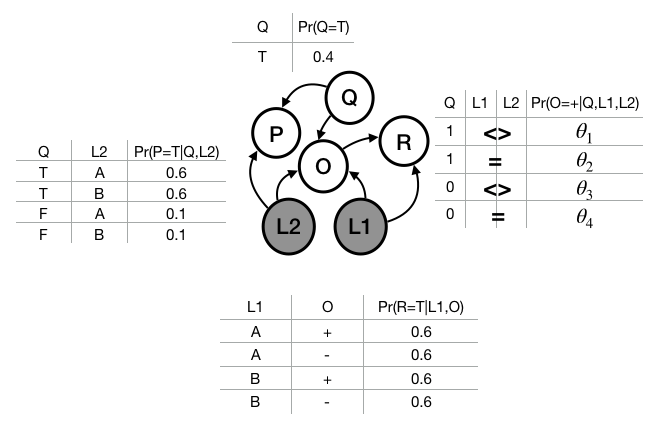
\includegraphics[width=\textwidth]{figs/BN.png}
  \end{minipage}\hfill
  \begin{minipage}[c]{0.45\textwidth}
    \caption{
        \small The model used for generating the datasets. There are four binary random variables, P, Q, O, and R. \textbf{P}: indicates whether or not the employee has high performance; \textbf{Q}: indicates whether or not an employee has high qualification; \textbf{O}: indicates whether or not the colleague submits the positive opinion towards the employee;  \textbf{R}: indicates whether or not the colleague has a positive opinion towards the employee;  \textbf{L1, L2}: indicates the label of the review provider and review receiver (observed).
    } \label{fig:BN}
  \end{minipage}
\end{figure}

We show the effectiveness of FairPSL by performing an empirical evaluation. We investigate two research questions in our experiments:
\begin{description}
\item[Q1] What is the effect of the fairness threshold $\delta$ on the fairness measures $RD/RC/RR$?
\item[Q2] How is decision quality affected by imposing $\delta$-fairness constraints?
\end{description}

Note that although we present the result for specific parameters of the framework in this section, we ran extensive analysis and the results we present are representative. We implemented the MAP inference routines of PSL and FairPSL in Python, using Gurobi-8.1\footnote{\url{www.gurobi.com}} as the backend solver. The FairPSL code, code for the data generator and data is publicly available\footnote{https://github.com/gfarnadi/FairPSL}. 

\subsection{Data generation}
  
We evaluate the FairPSL inference algorithm on synthetic datasets representing the performance review scenario (introduced in Example~\ref{ex:review}). The organization hierarchy is generated synthetically. 
The organization hierarchy generator is parameterized by two numbers: the number of employees in the organization ($n$) and the number of employees managed by each manager ($k$). Each employee is randomly assigned with a label \emph{A} or \emph{B}. An examples organization hierarchy with $n$=50 and $k$=3 is shown in Figure~\ref{fig:hierachy}.

\begin{figure}
  \begin{minipage}[c]{0.3\textwidth}
    \caption{
        \small An example of an organizational hierarchy with five levels and 50 employees with k=3. Each employee either has label A (shown with grey) or B (shown with white).
    }\label{fig:hierachy} 
	\end{minipage} \hfill
    \begin{minipage}[c]{0.7\textwidth}
    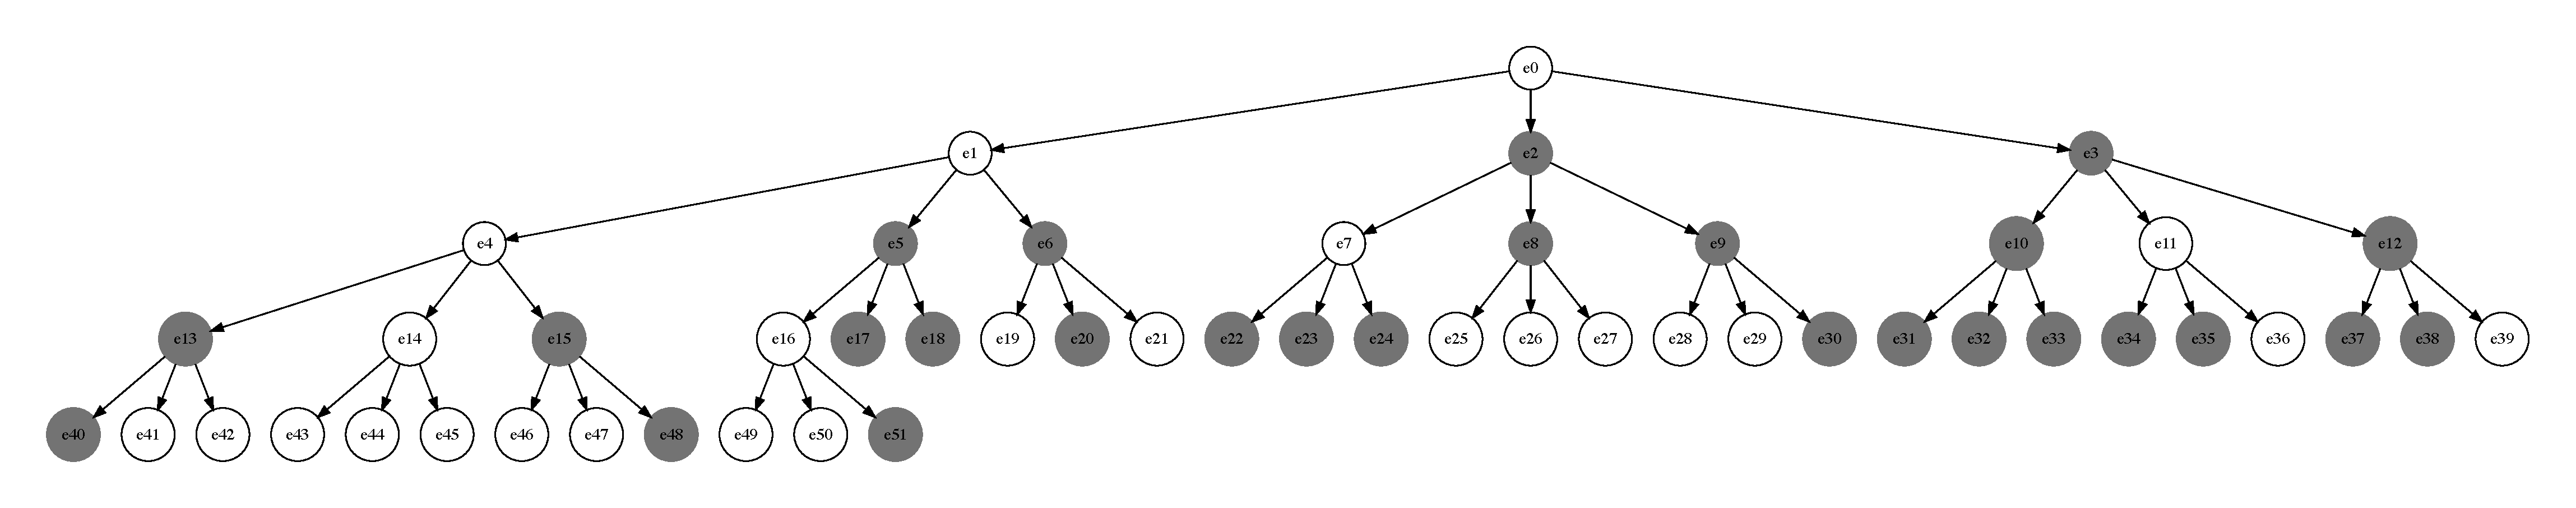
\includegraphics[width=\textwidth]{figs/Uni-hierachy.pdf}
  \end{minipage}
\end{figure}

For each employee, we use the generative model of Figure~\ref{fig:BN} to draw assignments for all the random variables. We assume that only $40\%$ of employees are qualified for promotion and regardless of their labels, employees submit only $60\%$ of their opinions. In addition, due to various personal and environmental factors, only $60\%$ of high quality employees perform well while $10\%$ of low quality employees also perform well regardless of their labels. Note that these numbers are not specific and just chosen for the framework to serve as a representative setting and a proof of concept. The conditional probability table for the opinion variable $O$ is parameterized by four values $(\theta_1, \theta_2, \theta_3, \theta_4)$ which together determine the degree of discrimination against the protected group. Since other parameters in the Bayesian network did not have a direct effect on the degree of discrimination, we fixed them to arbitrary values. 

The results presented in this section are based on an organization hierarchy  with $100$ employees where $k=5$. However, the results of the framework are not sensitive to the settings as we test the framework with various organization sizes ranging from $50$ to $500$ employees and various degree for $k$ ranging from $3$ to $10$. We generated seven datasets given the organization hierarchy using different values for the $\theta$ parameters: $(0.0,1.0,0.0,0.0)$, $(0.33,1.0,0.0,0.0)$, $(0.66,1.0,0.0,0.0)$, $(1.0,1.0,0.0,0.0)$, $(1.0,1.0,0.0,0.33)$, $(1.0,1.0,0.0,0.66)$, $(1.0,1.0,0.0,1.0)$. 
 
In the first three settings the discrimination originates from negative opinions towards qualified outgroup employees. The first setup is an extreme case where the opinion towards outgroup employees is always negative. The discrimination in the last three settings originates from positive opinions towards unqualified ingroup employees. The last setup is an extreme case where the opinion towards ingroup employees is always positive. The fourth setup represent unbiased opinions where employees are treated similarly based on their qualification. 

\paragraph{MAP Inference} We use the model presented in Table~\ref{tab:pslmodel} for MAP inference in PSL and FairPSL (recall that in FairPSL, the $\delta$-fairness constraints corresponding to one of the fairness measures are also added to the model). The observed atoms are $\textit{Manager(m,e)}$, $\textit{PositiveReview(e1,e2)}$ and labels of all employees. The truth values for all other atoms are obtained via MAP inference. We use the truth values obtained for the decision atoms $\textit{ToPromote(e)}$ to compute the fairness measures. We defined the discriminative pattern, and the protected and unprotected groups of this problem in Section~\ref{sec:formulation}.


\subsection{Evaluation results}

\begin{figure}
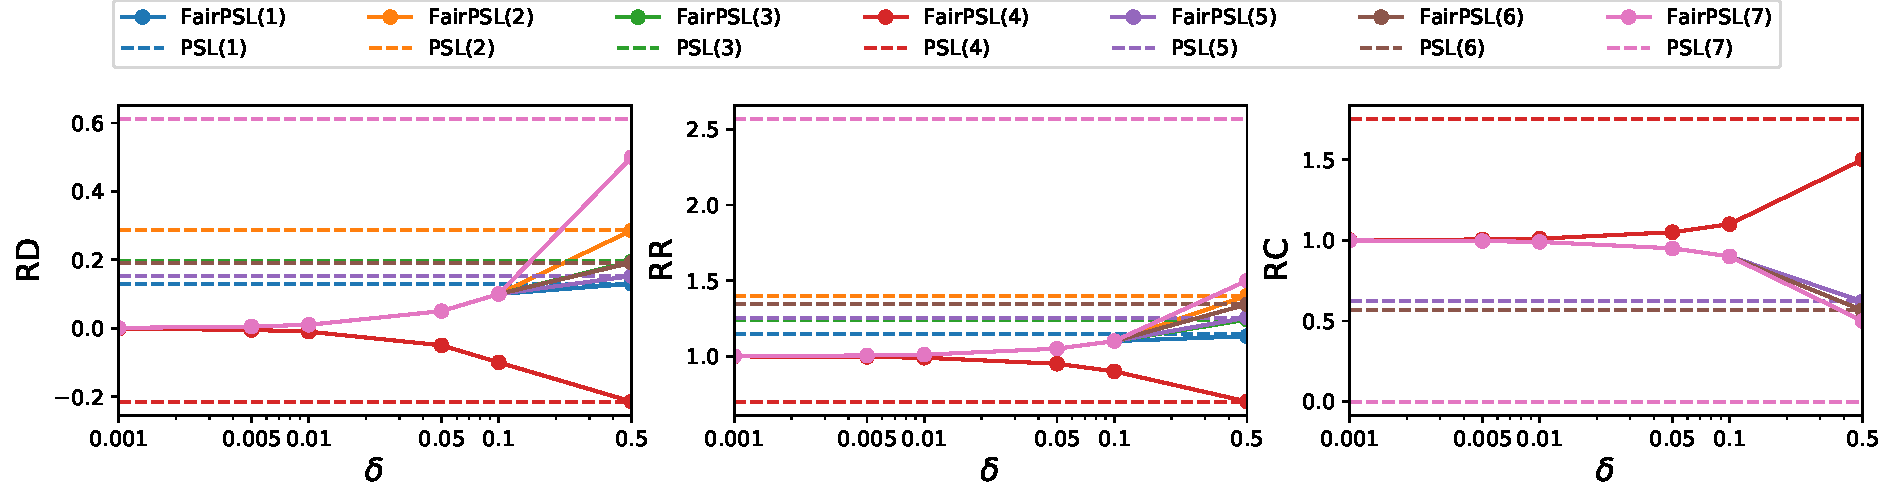
\includegraphics[width=1\linewidth]{figs/results_vis_uni_params.pdf}
\caption{\small Fairness score of predictions obtained by MAP inference of PSL and FairPSL, according to the fairness measures \emph{RD}, \emph{RR}, and \emph{RC}. The labels of datasets are mentioned with parenthesis next to the inference method. The FairPSL values of each measure are obtained by adding the $\delta$-fairness constraint of that measure.\label{fig:results}
}  
\end{figure}

To answer \textbf{Q1}, we run the MAP inference algorithm of PSL and FairPSL on seven synthetic datasets. 
We run the MAP inference of FairPSL multiple times on each dataset: For each of the three fairness measures, we add the corresponding $\delta$-fairness constraint with five thresholds $\{0.001, 0.005, 0.01, 0.05, 0.1, 0.5\}$.

Figure~\ref{fig:results} shows the fairness score of predictions in terms of the three fairness measures. As expected, tighter $\delta$-fairness constraints lead to better scores. Note that the best possible score according to RD is 0, as it computes a difference. Since RR and RC compute ratios, the best possible score according to these measures is 1. In our experiments, with any of these measures, taking $\delta = 0.001$ pushes the score of predictions to its limit.  

The $\delta$-fairness constraints modify the optimization problem of MAP inference by reducing the feasible region to solutions that conform with fairness guarantees. Research question \textbf{Q2} is concerned with the effect of this reduction on the accuracy of predictions. Note that decision quality is the same as the accuracy of predictions. To answer this question, we compare the inferred values for the decision atoms \textit{ToPromote(e)} against their actual values. These values are extracted from the known values of \textit{IsQualified(e)} according to rules 11 and 12 in Table~\ref{tab:pslmodel}. Figure~\ref{fig:accuracy} shows the area under the curve of the receiver operating characteristic~(AUC) of predicting the decision variable in three groups, namely the protected group, the unprotected group (i.e., promotion of the employees who have in-group managers), and all employees. By doing so, we make sure that our fairness constraints do not propagate bias towards either of the populations. Since the results of FairPSL with $\delta$-fairness constraints RR and RC are very similar to the results of RD, we only report the latter here.


\begin{figure}
    \centering
    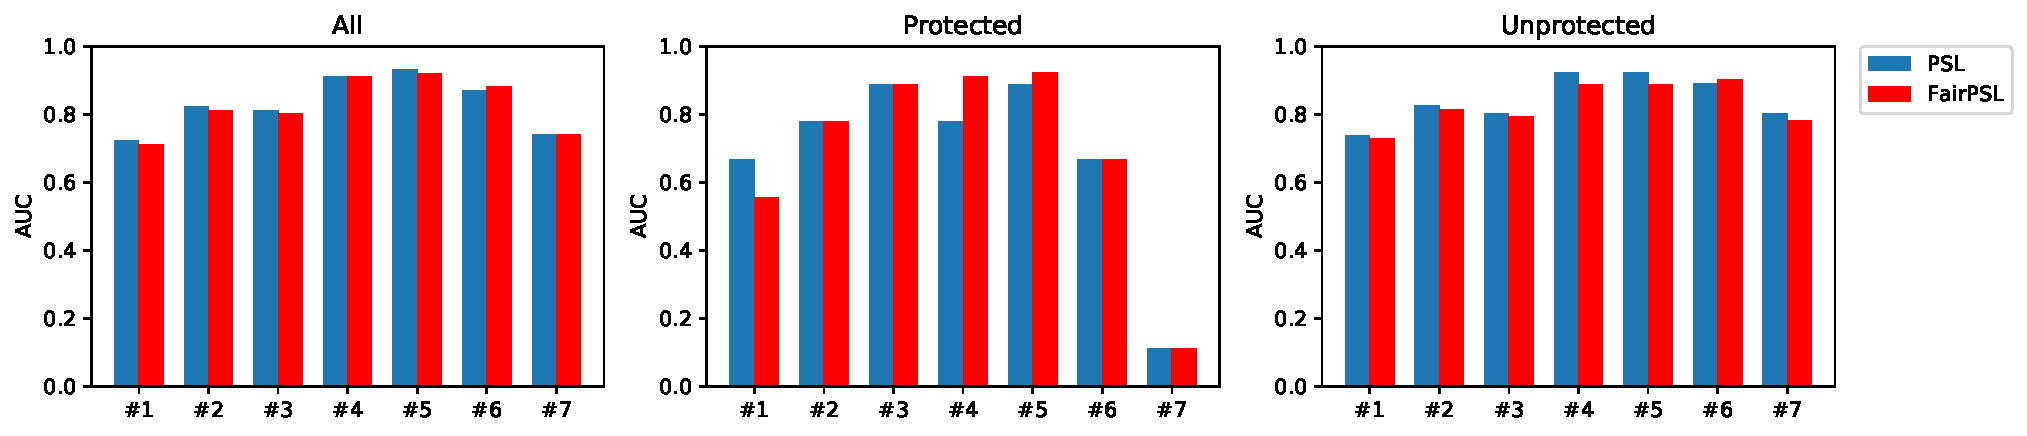
\includegraphics[width=\textwidth]{figs/roc.pdf}
    \caption{\small AUC score of predictions for truth values of unknown atoms \textit{ToPromote(e)} using MAP inference of PSL and FairPSL with $\delta$-fairness constraints $RD$ with $\delta=0.001$.}
    \label{fig:accuracy}
\end{figure}

According to Figure~\ref{fig:accuracy}, the results of both PSL and FairPSL in all seven datasets are close to each other. Note that although fairness may impose a cost in terms of overall accuracy, FairPSL often improves the accuracy of the protected class. Sometimes the overall predictions of FairPSL are even slightly better than PSL (e.g., dataset 6 and 7). As expected, the accuracy of the fourth setting where the opinions are unbiased are similar in both PSL and FairPSL. We observe that prediction of MAP inference for both FairPSL and PSL are similar, thus, in these settings at least, FairPSL guarantees fairness without hurting accuracy. Further investigation is required on the effect of the various ranges of discrimination (i.e., $\theta_1$, $\theta_2$, $\theta_3$, $\theta_4$) on the prediction results of FairPSL.



We also generate various types of organizations in which labels are not uniformly distributed, e.g., one population only occurs at the bottom levels of an organization. While we did not observe any differences in the behavior of our method with respect to accuracy and fairness measure, we found that the degree of discrimination is higher in such organizations. Further investigations on the structure of an organization on discrimination is an interesting direction for future research. 

\section{Conclusion and Future Directions}
\label{sec:conclusion}
Many applications of AI and machine learning affect peoples' lives in important ways. While there is a growing body of work on fairness in AI and ML, it assumes an individualistic notion of fairness.   In this paper, we have proposed a general framework for relational fairness which includes both a rich language for defining discrimination patterns and an efficient algorithm for performing inference subject to fairness constraints. We show our approach enforces fairness guarantees while preserving the accuracy of the predictions. 

There are many avenues for expanding on this work. For example, here we assumed that the discriminative pattern is given, however an automatic mechanism to extract discriminatory situations hidden in a large amount of decision records is an important and required task. Discrimination discovery has been studied for attribute-based fairness~\cite{pedreschi2013discovery}. An interesting next step is discrimination pattern discovery in relational data.

\section*{Acknowledgements}
This work is supported by the National Science Foundation under Grant Numbers CCF-1740850 and IIS-1703331. Golnoosh Farnadi and Behrouz Babaki are  supported by postdoctoral scholarships from IVADO through the Canada First Research Excellence Fund (CFREF) grant.

\begin{thebibliography}{10}
\itemsep=1pt 
\begin{small}

\bibitem{EUlaw}
European union legislation. (a) racial equality directive, 2000; (b) employment
  equality directive, 2000; (c) gender employment directive, 2006; (d) equal
  treatment directive (proposal), 2008.

\bibitem{UKlaw}
{UK} legislation. (a) sex discrimination act, 1975, (b) race relation act,
  1976.

\bibitem{USlaw}
United nations legislation. (a) universal declaration of human rights, 1948,
  (c) convention on the elimination of all forms of racial discrimination,
  1966, (d) convention on the elimination of all forms of discrimination
  against women, 1979.

\bibitem{alshukaili:iswc16}
Duhai Alshukaili, Alvaro A.~A. Fernandes, and Norman~W. Paton.
\newblock Structuring linked data search results using probabilistic soft
  logic.
\newblock In {\em International Semantic Web Conference {(1)}}, volume 9981 of
  {\em Lecture Notes in Computer Science}, pages 3--19, 2016.

\bibitem{bach:jmlr17}
Stephen~H. Bach, Matthias Broecheler, Bert Huang, and Lise Getoor.
\newblock Hinge-loss markov random fields and probabilistic soft logic.
\newblock {\em Journal of Machine Learning Research}, 18:109:1--109:67, 2017.

\bibitem{barocas2016big2}
Solon Barocas and Andrew~D Selbst.
\newblock Big data's disparate impact.
\newblock {\em California Law Review}, 104:671, 2016.

\bibitem{boyd2014networked}
Danah Boyd, Karen Levy, and Alice Marwick.
\newblock The networked nature of algorithmic discrimination.
\newblock In {\em Data and discrimination: Collected essays}, pages 53--57.
  2014.

\bibitem{brewer1979group}
Marilynn~B Brewer.
\newblock In-group bias in the minimal intergroup situation: A
  cognitive-motivational analysis.
\newblock {\em Psychological bulletin}, 86(2):307, 1979.

\bibitem{brewer2007social}
Marilynn~B Brewer.
\newblock The social psychology of intergroup relations: Social categorization,
  ingroup bias, and outgroup prejudice.
\newblock {\em Social Psychology: Handbook of Basic Principles}, 2007.

\bibitem{chouldechova2017fair2}
Alexandra Chouldechova.
\newblock Fair prediction with disparate impact: {A} study of bias in
  recidivism prediction instruments.
\newblock {\em CoRR}, abs/1703.00056, 2017.

\bibitem{dwork2012fairness3}
Cynthia Dwork, Moritz Hardt, Toniann Pitassi, Omer Reingold, and Richard~S.
  Zemel.
\newblock Fairness through awareness.
\newblock In {\em {ITCS}}, pages 214--226. {ACM}, 2012.

\bibitem{ebrahimi:emnlp16}
Javid Ebrahimi, Dejing Dou, and Daniel Lowd.
\newblock Weakly supervised tweet stance classification by relational
  bootstrapping.
\newblock In {\em {EMNLP}}, pages 1012--1017. The Association for Computational
  Linguistics, 2016.

\bibitem{farnadi2018fairness}
Golnoosh Farnadi, Behrouz Babaki, and Lise Getoor.
\newblock Fairness in relational domains.
\newblock In {\em AAAI/ACM Conference on AI, Ethics, and Society (AIES)}, pages
  108--114. ACM, 2018.

\bibitem{feldman2015certifying2}
Michael Feldman, Sorelle~A. Friedler, John Moeller, Carlos Scheidegger, and
  Suresh Venkatasubramanian.
\newblock Certifying and removing disparate impact.
\newblock In {\em {KDD}}, pages 259--268. {ACM}, 2015.

\bibitem{getoor2007introduction}
Lise Getoor and Ben Taskar.
\newblock {\em {Introduction to Statistical Relational Learning}}.
\newblock MIT press Cambridge, 2007.

\bibitem{hardt2016equality3}
Moritz Hardt, Eric Price, and Nati Srebro.
\newblock Equality of opportunity in supervised learning.
\newblock In {\em {NIPS}}, pages 3315--3323, 2016.

\bibitem{kamishima2011fairness}
Toshihiro Kamishima, Shotaro Akaho, and Jun Sakuma.
\newblock Fairness-aware learning through regularization approach.
\newblock In {\em ICDMW}, pages 643--650. {IEEE} Computer Society, 2011.

\bibitem{kouki:recsys15}
Pigi Kouki, Shobeir Fakhraei, James~R. Foulds, Magdalini Eirinaki, and Lise
  Getoor.
\newblock Hyper: {A} flexible and extensible probabilistic framework for hybrid
  recommender systems.
\newblock In {\em RecSys}, pages 99--106. {ACM}, 2015.

\bibitem{counterfactualfairness}
Matt~J. Kusner, Joshua~R. Loftus, Chris Russell, and Ricardo Silva.
\newblock Counterfactual fairness.
\newblock In {\em {NIPS}}, pages 4069--4079, 2017.

\bibitem{Pedreschi:2012}
Dino Pedreschi, Salvatore Ruggieri, and Franco Turini.
\newblock A study of top-k measures for discrimination discovery.
\newblock In {\em {SAC}}, pages 126--131. {ACM}, 2012.

\bibitem{pedreschi2013discovery}
Dino Pedreschi, Salvatore Ruggieri, and Franco Turini.
\newblock The discovery of discrimination.
\newblock In {\em Discrimination and Privacy in the Information Society},
  volume~3 of {\em Studies in Applied Philosophy, Epistemology and Rational
  Ethics}, pages 91--108. Springer, 2013.

\bibitem{ridgeway2004unpacking}
Cecilia~L Ridgeway and Shelley~J Correll.
\newblock Unpacking the gender system: A theoretical perspective on gender
  beliefs and social relations.
\newblock {\em Gender \& society}, 18(4):510--531, 2004.

\bibitem{sridhar:bioinformatics16}
Dhanya Sridhar, Shobeir Fakhraei, and Lise Getoor.
\newblock A probabilistic approach for collective similarity-based drug-drug
  interaction prediction.
\newblock {\em Bioinformatics}, 32(20):3175--3182, 2016.

\bibitem{verma2018fairness2}
Sahil Verma and Julia Rubin.
\newblock Fairness definitions explained.
\newblock In {\em 2018 IEEE/ACM International Workshop on Software Fairness
  (FairWare)}, pages 1--7. IEEE, 2018.

\bibitem{west2014exploiting}
Robert West, Hristo~S. Paskov, Jure Leskovec, and Christopher Potts.
\newblock Exploiting social network structure for person-to-person sentiment
  analysis.
\newblock {\em {TACL}}, 2:297--310, 2014.

\bibitem{zafar2017parity}
Muhammad~Bilal Zafar, Isabel Valera, Manuel Gomez{-}Rodriguez, Krishna~P.
  Gummadi, and Adrian Weller.
\newblock From parity to preference-based notions of fairness in
  classification.
\newblock In {\em {NIPS}}, pages 228--238, 2017.

\bibitem{zemel2013learning}
Richard~S. Zemel, Yu~Wu, Kevin Swersky, Toniann Pitassi, and Cynthia Dwork.
\newblock Learning fair representations.
\newblock In {\em {ICML} {(3)}}, volume~28 of {\em {JMLR} Workshop and
  Conference Proceedings}, pages 325--333. JMLR.org, 2013.

\end{small}
\end{thebibliography}

\end{document}

\end{article}



\begin{article}
{Ethical Challenges in the Future of Work}
{Pierre Bourhis, Gianluca Demartini, Shady Elbassuoni, Emile Hoareau, H. Raghav Rao}
\graphicspath{{submissions/automl/}}
%\documentclass[11pt,dvipdfm]{article}
\documentclass[11pt]{article}
\usepackage{deauthor,times,graphicx} %required
\usepackage{amsmath,amssymb}
\usepackage{multirow}
\usepackage{algorithm}
\usepackage{algpseudocode}
\usepackage{todonotes}
\usepackage{url}

% \graphicspath{{farnadi/}}

\newtheorem{mydef}{\textbf{Definition}}
\newtheorem{myex}{\textbf{Example}}
\newtheorem{mytheorem}{\textbf{Theorem}}


\begin{document}

\title{A Declarative Approach to Fairness in Relational Domains}
\author{Golnoosh Farnadi$^{1,2}$, Behrouz Babaki$^1$, Lise Getoor$^3$\\
$^1$Polytechnique Montr\'{e}al, $^2$ Mila, $^3$ UC Santa Cruz \\
farnadig@mila.quebec, behrouz.babaki@polymtl.ca, getoor@soe.ucsc.edu}

\maketitle

\begin{abstract}
AI and machine learning tools are being used with increasing frequency for decision making in domains that affect peoples' lives such as employment, education, policing and %loan approval
financial qualifications. These uses raise concerns about biases of algorithmic discrimination and have motivated the development of fairness-aware machine learning. However, existing fairness approaches are based solely on attributes of individuals. In many cases, discrimination is much more complex, and taking into account the social, organizational, and other connections between individuals is important. We introduce new notions of fairness that are able to capture the relational structure in a domain. We use first-order logic to provide a flexible and expressive language for specifying complex relational patterns of discrimination. Furthermore, we extend an existing statistical relational learning framework, probabilistic soft logic~(PSL), to incorporate our definition of relational fairness. We refer to this fairness-aware framework FairPSL. FairPSL makes use of the logical definitions of fairnesss but also supports a probabilistic interpretation. In particular, we show how to perform maximum a posteriori~(MAP) inference by exploiting probabilistic dependencies within the domain while avoiding violations of fairness guarantees. Preliminary empirical evaluation shows that we are able to make both accurate and fair decisions.
\end{abstract}

\section{Introduction}
\label{sec:introduction}

Over the past few years, AI and machine learning have become essential components in operations that drive the modern society, e.g., in financial, administrative, and educational spheres. \emph{Discrimination} happens when qualities of individuals which are not relevant to the decision making process influence the decision. Delegating decision making to an automated process raises questions about discriminating against individuals with certain traits based on biases in the data. This is especially important when the decisions have the potential to impact the lives of individuals, for example, the decisions on granting loans, assigning credit, and employment. 

\emph{Fairness} is defined as the absence of discrimination in a decision making process. The goal of \emph{fairness-aware} machine learning is to ensure that the decisions made by an algorithm do not discriminate against a population of individuals~\cite{feldman2015certifying2,boyd2014networked,hardt2016equality3}. Fairness has been well studied in the social sciences and legal scholarship (for an in-depth review see~\cite{barocas2016big2}), and there is emerging work on fairness-aware ML within the AI and computer science communities. For example, fairness through awareness/Lipschitz property~\cite{dwork2012fairness3}, individual fairness~\cite{zemel2013learning}, statistical parity/group fairness~\cite{kamishima2011fairness}, counterfactual fairness~\cite{counterfactualfairness}, demographic parity/disparate impact~\cite{feldman2015certifying2,chouldechova2017fair2}, preference-based fairness~\cite{zafar2017parity}, and equality of opportunity~\cite{hardt2016equality3}.

The existing work in fairness-aware machine learning is based on a definition of discrimination where a decision is influenced by an \emph{attribute} of an individual. An attribute value upon which discrimination is based (such as gender, race, or religion) is called a \emph{sensitive attribute}. The sensitive attribute defines a population of vulnerable individuals known as the \emph{protected group}. A fair decision-making process treats the protected group the same as the \emph{unprotected group}. 

However, in many social contexts, discrimination is the result of complex interactions and can not be described solely in terms of attributes of an individual. For example, consider an imaginary scenario in an organization in which younger female workers who have older male supervisors have lower chances of promotion than their male counterparts.\footnote{Of course, many other patterns may be possible: female bosses may promote female subordinates and discriminate against male workers, or male bosses may promote female employees.  Our goal is to provide a general framework which is able to describe arbitrarily complex discrimination patterns.} 
 This discrimination pattern involves two attributes of the individual (gender and age), a relationship with another individual (supervisor), and two attributes of the second individual. Addressing such complex cases poses two challenges. First, the concepts of discrimination and fairness need to be extended to capture not only attributes of individuals but also the relationships between them. Second, a process is required that ensures that fair decisions are made about individuals who are affected by such patterns. In this paper we address both of these challenges.
We use first-order logic (FOL) to extend the notion of fairness to the relational setting. FOL is an expressive representation for relational problems which is also widely used for learning in relational domains. Moreover, we extend an existing framework for statistical relational learning~\cite{getoor2007introduction} called probabilistic soft logic (PSL)\footnote{http://psl.linqs.org/}~\cite{bach:jmlr17}. PSL combines logic and probability for learning and reasoning over uncertain relational domains. One of the most common reasoning tasks in PSL is called maximum a posteriori (MAP) inference, which is performed by finding the most probable truth values for unknowns over a set of given evidence. We develop a new MAP inference algorithm which is able to maximize the a posteriori values of unknown variables \emph{subject to} fairness guarantees. An early version of this paper which this work builds upon and extends appeared in~\cite{farnadi2018fairness}.

\looseness-1
Our contributions are as follows: 1) we propose fairness-aware machine learning for the relational setting; 2) we extend PSL into a fairness-aware framework called FairPSL which can represent the logical definition of fairness; 3) we develop a new MAP inference algorithm which is able to maximize the posteriori values of unknown variables \emph{subject to} fairness guarantees; 4) we empirically evaluate our proposed framework on synthetic data. 

\section{Motivation}
\label{sec:motivation}

Discrimination in social contexts have been studied in the field of social psychology~\cite{brewer2007social,brewer1979group,ridgeway2004unpacking}. There is a large literature on various aspects of relational bias in social contexts such as \emph{in-group-out-group bias}, \emph{gender bias}, and \emph{ethnicity-based favoritism} that can result in discrimination. 
As an example, consider gender bias in the workplace that reflects stereotypically masculine criteria and male-based favoritism. Such gender bias 
typically places women in lower positions and negatively impacts their opportunities. Further, lack of women in leadership positions may affect the promotion of women and results in a glass ceiling that keeps women from rising beyond a certain level in the hierarchy. This scenario shows that considering  protected attributes such as gender is not always sufficient to detect the source of bias and avoid discrimination, one also has to consider the relational information, in this case the organization hierarchy. Note that this can be generalized to any ingroup/outgroup scenario where the sensitive attribute could be race, religion, age, marital-status, etc.

The existing work on designing fair algorithms in machine learning exclusively focuses on \emph{attribute-based fairness}, which is based on the following assumptions: First, there is an assumption that the individuals (sometimes referred to as units or entities) are independent and described by simple attribute vectors. Second, the group for which one wishes to ensure fairness (known as the \emph{protected group}) is defined on the basis of some attribute values. Finally, there is a decision that is associated with each individual, and the goal is to ensure that members of the protected group are subject to a fair decision (we discuss different fairness measures in Section~\ref{sec:fairnessmeasure}).  We illustrate  attribute-based fairness in the following example. 

\begin{myex}[Loan Processing]
\label{ex:loan}
A bank bases its decisions about granting a loan on attributes of the applicant. The goal is to decide whether to grant a loan to an applicant using a predictive model. The bank needs to ensure that the obey fair lending practices and ensure that gender, race, sexual orientation of applicants has no influence on the decision. In this scenario, the protected group is the historically disadvantaged applicants.  
\end{myex}
The current fairness-aware machine learning techniques are not capable of modeling relations and hence cannot be used to make the decision making model fair. However, in many decision making scenarios, especially in social and organizational settings, the domain is relational, and the protected group itself might be best represented using a relational definition. We illustrate this setting in the following scenario:
\begin{myex}[Performance Review]
\label{ex:review}
Consider an organization where decisions about the promotion of employees is based on two criteria: 1) an objective performance measure, and 2) the opinion of their direct and indirect managers above them. The opinions are inferred from the performance reviews which are collected periodically. Not every manager can submit a review for all its subordinates, this is especially the case for top-level managers who have a large number of subordinates. Hence, the opinions of managers are collectively inferred from the opinions of their sub-ordinates. However, some employees may be biased, and judge other employees unfavorably, by favoring employees who are similar to themselves (same gender, race, religion, etc.) over employees who are dissimilar. The organization needs to ensure that promotion of employees do not have any relational bias caused by in-group-out-group favoritism.

\end{myex}
Example~\ref{ex:review} describes a prediction problem over a database that consists of relations between employees. Such prediction tasks are best handled by techniques from the relational learning domain. To ensure fair prediction in such settings, we need to extend the notion of \emph{attribute-based fairness} to \emph{relational fairness}. Throughout this paper, we use the performance review problem as a running example for relational fairness.

\section{Fairness Formalism}
\label{sec:formulation}

A representation that can describe different types of entities and different relationships between them is called relational. In this section, we use first-order logic to define relational fairness. We employ first-order logic as an expressive representation formalism which can represent objects and complex relationships between them. We start by defining an atom:

\begin{mydef}[Atom]
An atom is an expression of the form $P(a_1, a_2, \ldots, a_n)$ where each argument $a_1, a_2,$ $\ldots,$ $a_n$ is either a constant or a variable. The finite set of all possible substitutions of a variable to a constant for a particular variable $a$ is called its \textit{domain} $D_{a}$. If all variables in $P(a_1, a_2, \ldots, a_n)$ are substituted by some constant from their respective domain, then we call the resulting atom a \textit{ground atom}. 
\end{mydef}

\begin{myex}
In our loan processing problem (Example~\ref{ex:loan}), we can represent applicants' attributes by atoms. For instance, atom $Female(v)$ indicates whether or not applicant $v$ is female. Similarly, we can represent relations with atoms. In the performance review problem in Example~\ref{ex:review} the atom $Manager(m,e)$ indicates whether or not employee $m$ is a direct or indirect manager of employee $e$.
\end{myex}

The relational setting provides the flexibility to express complex definitions with formulae.

\begin{mydef}[Formula] 
A formula is defined by induction: every atom is a formula. If $\alpha$ and $\beta$ are formulae, then $\alpha \vee \beta$, $\alpha \wedge \beta$, $\neg \alpha$, $\alpha \rightarrow \beta$ are formulae. If $x$ is a variable and $\alpha$ is a formula, then the quantified expressions of the form $\exists x$ $\alpha$ and $\forall x$ $\alpha$ are formulae.    
\end{mydef}

To characterize groups of individuals based on a formula, we define the notion of \emph{population}.

\begin{mydef}[Population]
We denote formula $F$ which has only one free variable $v$ (i.e., other variables in $F$ are quantified) by $F[v]$. The population defined by $F[v]$ is the set of substitutions of $v$ for which $F[v]$ holds.   
\end{mydef}


\begin{myex}
\label{ex:disformula}
Consider the formula $F[v] := \forall u, \, \textit{Manager}(u,v) \rightarrow \neg \textit{SameGroup}(u, v)$. The population specified by this formula is the set of individuals all of whose managers belong to a group different from theirs. 
\end{myex}

The truth value of a formula is derived from the truth value of atoms that it comprises, according to the rules of logic. Each possible assignment of truth values to ground atoms is called an \emph{interpretation}. 


\begin{mydef}[Interpretation]
An interpretation $I$ is a mapping that associates a truth value $I(P)$ to each ground atom $P$. For Boolean truth values, $I$ associates true to 1 and false to 0 truth values. For soft logic (see Definition~\ref{def:softlogic}) $I$ maps each ground atom $P$ to a truth value in interval $[0, 1]$.
\end{mydef}

In attribute-based fairness, it is assumed that there is a certain attribute of individuals, i.e, the sensitive attribute,  that we do not want to affect a decision. Gender, race, religion and marital status are examples of sensitive attributes. Discrimination has been defined in social science studies as a treatment in favor or against a group of individuals given their sensitive attribute. This group of individuals is the protected group. 

In a relational setting, both the sensitive attributes of an individual and their participation in various relations may have an undesired effect on the final decision. We characterize the protected group in a relational setting by means of a population. In practice, we are often interested in maintaining fairness for a specific population such as applicants, students, employees, etc. This population is then partitioned into the protected and unprotected groups. We define a \emph{discriminative pattern} which is a pair of formulae to capture these groups: 1) $F_1[v]$: to specify the difference between the protected and unprotected groups and 2) $F_2[v]$: to specify the population over which we want to maintain fairness. 

\begin{mydef}[Discriminative pattern]
A discriminative pattern is a pair $\textit{DP}[v]:=(F_1[v], F_2[v])$ , where $F_1[v]$ and $F_2[v]$ are formulae.
\end{mydef}

\begin{myex}
\label{ex:pattern}
The two formulae in the discrimination pattern $\textit{DP}[v]:= \big((\forall u, \,  \textit{Manager}(u,v) \rightarrow  \neg \textit{SameGroup}(u, v)),$ $\textit{Employee}(v)\big)$ specify two populations, namely all employees and those employees who belong to a group different from their managers.
\end{myex}

Given the definition of the discriminative pattern, we have a rich language to define the scope of the protected and unprotected groups in a relational setting.

\begin{mydef}[Protected group] Given an interpretation $I$, the protected group is a population of the form:
{$$PG :=\{ v : F_1[v] \wedge F_2[v]\}$$}
which is defined as the set of all instances hold for variable $v$ for which $F_1[v] \wedge F_2[v]$ is true under interpretation $I$, that is, $I(F_1[v] \wedge F_2[v]) = 1$. 
Similarly, the \emph{unprotected group} is a population of the form: 
{$$UG := \{ v : \neg F_1[v] \wedge  F_2[v]\}$$}
which is defined as the set of all instances hold for variable $v$ 
for which $I(\neg F_1[v] \wedge F_2[v]) = 1$. 
\end{mydef}

\begin{myex}
The protected group of the discrimination pattern specified in Example~\ref{ex:pattern} is {$PG := \big\{ v : \big(\forall u, \,$ $ \textit{Manager}(u, v) \rightarrow \neg \textit{SameGroup}(u, v)\big) \wedge \textit{Employee}(v) \big\}$} and the unprotected group is {$UG :=  \big\{ v:  \big(\exists u, \, \textit{Manager}(u,v) \wedge \textit{SameGroup}(u, v)\big) \wedge \textit{Employee}(v) \big\}$}. This means our protected group is the set of employees belonging to a group different from their managers,
and our unprotected group consists of other employees. 
\end{myex}

Discrimination is defined in terms of a treatment or decision that distinguishes between the protected and unprotected groups. Here we define the \emph{decision} atom.
\begin{mydef}[Decision atom] A decision atom $d(v)$ is an atom containing exactly one variable $v$ that specifies a decision affecting the protected group which is defined either by law or end-user.
\end{mydef}
\begin{myex}
The decision atom ${\textit ToPromote}(v)$ indicates whether or not $v$ receives a promotion.
\end{myex}

Note that the fairness formulation in this section is designed for the relational setting, however relational fairness subsumes the attribute-based fairness such that: a sensitive attribute is defined by an atom with one argument and $F_2[v]$ in discrimination pattern is $\textit{Applicant}(v)$. For example, discrimination pattern of our loan processing problem in Example~\ref{ex:loan} is of the form $\textit{DP} := ( \textit{Female}(v), \textit{Applicant}(v))$ that denotes female applicants as the protected group (i.e., $PG :=  \{ v: \textit{Female}(v) \}$) and male applicants as the unprotected group (i.e., $UG := \{ v: \neg \textit{Female}(v)\}$).


\section{Fairness Measures}
\label{sec:fairnessmeasure}

Over the past few years, many fairness measures have been introduced~\cite{verma2018fairness2}. An important class of these measures are \emph{group fairness} measures which quantify the inequality between different subgroups. Some of the most popular measures in this class include \emph{equal opportunity}, \emph{equalized odds}, and \emph{demographic parity}~\cite{hardt2016equality3}. In this paper we restrict our focus to the latter. In an attribute-value setting, demographic parity means that the decision should be independent of the protected attributes. Assume that binary variables $A$ and $C$ denote the decision and protected attributes, and the preferred value of $A$ is one. Demographic parity requires that:

\begin{equation*}
    P(A=1 | C=0) = P(A=1 | C=1)
\end{equation*}

We will now generalize this measure to the relational setting using the notations defined in Section~\ref{sec:formulation}. Let $a$ and $c$ denote the counts of denial (i.e., negative decisions) for protected and unprotected groups, and $n_{1}$ and $n_{2}$ denote their sizes, respectively. Given the decision atom $d(v)$, discriminative pattern $\textit{DP}(F_1[v], F_2[v])$, and interpretation $I$, these counts are computed by the following equations: 
{
\begin{flalign}
    & a \equiv \sum_{v \in D_v} I\big( \neg d(v) \wedge  F_1[v] \wedge F_2[v]) \label{eq:a}\\
    & c \equiv \sum_{v \in D_v} I\big( \neg d(v) \wedge  \neg F_1[v] \wedge  F_2[v]) \label{eq:c}\\
    & n_{1} \equiv \sum_{v \in D_v} I\big(F_1[v] \wedge F_2[v]) \label{eq:n1}\\
    & n_{2} \equiv \sum_{v \in D_v} I\big(\neg F_1[v] \wedge  F_2[v]) \label{eq:n2}
\end{flalign}}
The proportions of denying for protected and unprotected groups are $p_1 = \frac{a}{n_1}$ and $p_2 = \frac{c}{n_2}$, respectively. There are a number of data-driven measures~\cite{Pedreschi:2012} which quantify demographic disparity and can be defined in terms of $p_1$ and $p_2$:
\begin{itemize}
    \item \textbf{Risk difference}: $RD = p_1 - p_2$, also known as absolute risk reduction. 
    \item \textbf{Risk Ratio}: $RR = \frac{p_1}{p_2}$, also known as relative risk. 
    \item \textbf{Relative Chance}: $RC = \frac{1 - p_1}{1 - p_2}$ also, known as selection rate.
\end{itemize}
These measures have been used in the legal systems of European Union, UK, and US~\cite{EUlaw,UKlaw,USlaw}. Notice that RR is the ratio of the proportion of benefit denial between the protected and unprotected groups, while RC is the ratio of the proportion of benefit granted. Finally, we introduce the notion of $\delta$-fairness.

\begin{mydef}[$\delta$-fairness]
If a fairness measure for a decision making process falls within some $\delta$-window, then the process is \emph{$\delta\text{-fair}$}. Given $0 \leq \delta \leq 1$, the  $\delta$-windows for measures RD/RR/RC are defined as:
{\begin{flalign*}
	     - \delta \leq &RD \leq \delta \\
	     1- \delta \leq &RR \leq 1+ \delta\\
	     1- \delta \leq &RC \leq 1+ \delta
	\end{flalign*}}
\end{mydef}

To overcome the limitations of attribute-based fairness, we introduce a new statistical relational learning~(SRL) framework~\cite{getoor2007introduction} suitable for modelling fairness in relational domain. In the next section, we review probabilistic soft logic~(PSL). We then extend PSL with the definition of relational fairness introduced above in Section~\ref{sec:fairMAP}. Our fairness-aware framework, ``FairPSL'', is the first SRL framework that performs fair inference. 

\section{Background: Probabilistic Soft Logic}
\label{sec:psl}

In this section, we review the syntax and semantics of PSL, and in the next section we extend MAP inference in PSL with fairness constraints to define MAP inference in FairPSL.

PSL is a probabilistic programming language for defining hinge-loss Markov random fields~\cite{bach:jmlr17}. Unlike other SRL frameworks whose atoms are Boolean, atoms in PSL can take continuous values in the interval $[0,1]$. PSL is an expressive modeling language that can incorporate domain knowledge with first-order logical rules and has been used successfully in various domains, including bioinformatics~\cite{sridhar:bioinformatics16}, recommender systems~\cite{kouki:recsys15}, natural language processing~\cite{ebrahimi:emnlp16}, information retrieval~\cite{alshukaili:iswc16}, and social network analysis~\cite{west2014exploiting}, among many others. 
 
A PSL model is defined by a set of first-order logical rules called \emph{PSL rules}.

\begin{mydef} [PSL rule] a PSL rule $r$ is an expression of the form:
{\begin{equation}
\lambda_{r}: T_1 \land T_2 \land \ldots \land T_w \rightarrow H_1 \vee H_2 \vee \ldots \vee H_l
\end{equation}}

where { $T_1, T_2, \ldots, T_w, H_1, H_2, \ldots, H_l$} are atoms or negated atoms and { $\lambda_{r} \in \mathbb{R}^{+} \cup \infty$} is the weight of the rule $r$.  We call { $T_1 \land T_2 \land \ldots \land T_w$} the body of $r$ ($r_{body}$), and { $H_1 \vee H_2 \vee \ldots \vee H_l$} the head of $r$ ($r_{head}$).
\end{mydef}


Since atoms in PSL take on continuous values in the unit interval $[0,1]$, next we define soft logic to calculate the value of the PSL rules under an interpretation $I$.

\begin{mydef}[Soft logic]
\label{def:softlogic}
The ({$\tilde{\wedge}$}) and ({$\tilde{\vee}$}) and negation ({$\tilde{\neg}$}) are defined as follows. For {$m, n \in [0,1]$} we have: {$m \tilde{\wedge} n = \max(m+n -1, 0)$}, {$m \tilde{\vee} n = \min(m+n , 1)$} and {$\tilde{\neg} m = 1 - m$}. The $\, \tilde{} \,$ indicates the relaxation over Boolean values.
\end{mydef}

The probability of truth value assignments in PSL is determined by the rules' \emph{distance to satisfaction}.

\begin{mydef}[The distance to satisfaction]
The distance to satisfaction $d_{r}(I)$ of a rule $r$ under an interpretation $I$ is defined as:
{
\begin{equation}
d_{r}(I) = \max\{0, I(r_{body})-I(r_{head})\}
\end{equation}}
\end{mydef}

By using Definition~\ref{def:softlogic}, one can show that the closer the interpretation of a grounded rule $r$ is to 1, the smaller its distance to satisfaction. A PSL model induces a distribution over interpretations $I$. Let $R$ be the set of all grounded rules, then the probability density function is:
{
\begin{equation}
f(I) ={\frac{1}{Z}} \exp[-\sum_{r\in R} \lambda_{r}(d_{r}(I))^p]
\label{eq:potential}
\end{equation}
}
\noindent where { $\lambda_{r}$} is the weight of rule $r$, {
$Z = \int_{I} \exp[ -\sum_{r\in R} \lambda_{r}(d_{r}(I))^p]$
} is a normalization constant, and { $p \in \{1,2\}$} provides a choice of two different loss functions, $p=1$ (i.e., linear), and $p=2$ (i.e, quadratic). These probabilistic models are instances of hinge-loss Markov random fields~(HL-MRF)~\cite{bach:jmlr17}. The goal of maximum a posteriori (MAP) inference is to find the most probable truth assignments $I_{\textit{MPE}}$ of unknown ground atoms given the evidence which is defined by the interpretation $I$. Let $X$ be all the evidence, i.e., $X$ is the set of ground atoms such that $\forall x \in X, I(x)$ is known, and let $Y$ be the set of ground atoms such that $\forall y \in Y, I(y)$ is unknown. Then we have
{
\begin{equation}
I_{\textit{MAP}}(Y) = \textit{arg}\max_{I(Y)} P(I(Y)|I(X))
\end{equation}}
Maximizing the density function in Equation~\ref{eq:potential} is equivalent to minimizing the weighted sum of the distances to satisfaction of all rules in PSL. 

\begin{table*}[t]
    \centering
    \begin{tabular}{|lll|}
    \hline
    &&\\
    $R1$ & $\lambda_1$ &: $\textit{IsQualified}(e) \rightarrow \textit{HighPerformance}(e)$ \\
    $R2$ & $\lambda_1$ &: $\neg \textit{IsQualified}(e) \rightarrow \neg \textit{HighPerformance}(e)$ \\
    $R3$ & $\infty$ &: $\textit{PositiveReview}(e1, e2) \rightarrow \textit{PositiveOpinion}(e1, e2)$ \\
    $R4$ & $\infty$ &: $\neg \textit{PositiveReview}(e1, e2) \rightarrow \neg \textit{PositiveOpinion}(e1, e2)$ \\
    $R5$ & $\lambda_1$ &: $\textit{PositiveOpinion}(e1, e2) \wedge \textit{Manager}(m, e1) \rightarrow \textit{PositiveOpinion}(m, e2)$ \\
    $R6$ & $\lambda_1$ &: $\neg \textit{PositiveOpinion}(e1, e2) \wedge \textit{Manager}(m, e1) \rightarrow \neg \textit{PositiveOpinion}(m, e2)$ \\
    $R7$ & $\lambda_1$ &: $\textit{PositiveOpinion}(m, e) \wedge \textit{Manager}(m, e) \rightarrow \textit{IsQualified}(e)$ \\
    $R8$ & $\lambda_1$ &: $\neg \textit{PositiveOpinion}(m, e) \wedge \textit{Manager}(m, e) \rightarrow \neg \textit{IsQualified}(e)$ \\
    $R9$ &  $\lambda_1$ &: $\neg \textit{ToPromote}(e)$\\
    $R10$ & $\infty$ &: $\textit{IsQualified}(e) \rightarrow \textit{ToPromote}(e)$ \\
    $R11$ & $\infty$ &: $\neg \textit{IsQualified}(e) \rightarrow \neg \textit{ToPromote}(e)$ \\
    &&\\
    \hline
    \end{tabular}
    \caption{\small A simplified PSL model for the \emph{Performance Reviewing} problem}
    \label{tab:pslmodel}
\end{table*}

\begin{myex}
\label{ex:pslmodel}
The simplified PSL model for the performance reviewing problem in Example\ref{ex:review} is given in Table~\ref{tab:pslmodel}. The goal of MAP inference for this problem is to infer employees to promote. We simplified the model by assigning the same weight to all soft rules (i.e., $\lambda_i= 1$ where $i=\{1,2,5,6,7,8,9\}$). Below we explain the meaning of each rule in the model.

Rule $R1$ indicates that qualified employees have high performance and similarly rule $R2$ expresses that a negative qualification of employees is derived from their low performance. Rules $R5$ and $R6$ presents the propagation of opinion from bottom to top of the organizational hierarchy, i.e., managers have similar opinions towards employees given the opinions of their sub-ordinate managers. And rules $R7$ and $R8$ indicate that the positive/negative opinion of direct/indirect managers derive from the qualification of an employee. Rule $R9$ indicates the prior that not all employees get promoted. We also have four hard constraints (i.e., rules $R3$, $R4$, $R10$ and $R11$) where the weight of the rules are $\infty$. Rules $R3$ and $R4$ indicate that submitted positive/negative reviews should reflect positive/negative opinions. And two rules $R10$ and $R11$ show that a highly qualified employee should get promoted. 
\end{myex}

\section{Fairness-aware PSL (FairPSL)}
\label{sec:fairMAP}

The standard MAP inference in PSL aims at finding values that maximize the conditional probability of unknowns. Once a decision is made according to these values, one can use the fairness measure to quantify the degree of discrimination. A simple way to incorporate fairness in MAP inference is to add the $\delta$-fairness constraints to the corresponding optimization problem.   

Consider risk difference, $\textit{RD}$, where $\textit{RD} \equiv \frac{\mathbf{a}}{n_1} - \frac{\mathbf{c}}{n_2}$. The $\delta$-fairness constraint $-\delta \leq \textit{RD} \leq \delta$ can be encoded as the following constraints:
{\begin{align}
    & n_2 \mathbf{a} - n_1 \mathbf{c} - n_1 n_2 \delta \leq 0 \label{eq:RD1}\\
    & n_2 \mathbf{a} - n_1 \mathbf{c} + n_1 n_2 \delta \geq 0
\end{align}}
Similarly, from $\textit{RR} \equiv \frac{\mathbf{a} / n_1}{\mathbf{c} / n_2}$ and the $\delta$-fairness constraint $1 - \delta \leq \textit{RR} \leq 1 + \delta$ we obtain:
{\begin{align}
    & n_2 \mathbf{a} - (1 + \delta) n_1 \mathbf{c} \leq 0 \\
    & n_2 \mathbf{a} - (1 - \delta) n_1 \mathbf{c} \geq 0
\end{align}}
And finally, $\textit{RC} \equiv \frac{1 - \mathbf{a} / n_1}{1 - \mathbf{c} / n_2}$ and the $\delta$-fairness constraint $1 - \delta \leq \textit{RC} \leq 1 + \delta$ gives:
{ \begin{align}
    & - n_2 \mathbf{a} + (1 + \delta) n_1 \mathbf{c} - \delta n_1 n_2 \leq 0 \\
    & - n_2 \mathbf{a} + (1 - \delta) n_1 \mathbf{c} + \delta n_1 n_2 \geq 0 \label{eq:RC2}
\end{align}}
A primary advantage of PSL over similar frameworks is that its MAP inference task reduces to a convex optimization problem which can be solved in polynomial time. To preserve this advantage, we need to ensure that the problem will remain convex after the addition of $\delta$-fairness constraints. 

\begin{mytheorem}
The following condition is sufficient for preserving the convexity of MAP inference problem after addition of $\delta$-fairness constraints: The formulae $F_1[v]$ and $F_2[v]$ do not contain an atom $y \in Y$ and all atoms in $F_1[v]$ and $F_2[v]$ have values zero or one.
\end{mytheorem}
\begin{proof}
Since $I(F_1[v])$ and $I(F_2[v])$ do not depend on $I(Y)$, the values $n_{1}$ and $n_{2}$ are constants that can be computed in advance. Let us define the sets $D_v^a = \{ v \in D_v : F_1[v] \wedge F_2[v] \, \text{is true} \}$ and $D_v^c = \{ v \in D_v : \neg F_1[v] \wedge F_2[v] \, \text{is true} \}$. Since $F_1[v]$ and $F_2[v]$ can be only zero or one, we can rewrite the equations~\ref{eq:a} and \ref{eq:c} as:
{
\begin{align*}
    & \mathbf{a} = \sum_{v \in D_v^a} I(\neg d(v)) = |D_v^a| - \sum_{v \in D_v^a} I(d(v))\\
    & \mathbf{c} = \sum_{v \in D_v^c} I(\neg d(v)) = |D_v^c| - \sum_{v \in D_v^c} I(d(v))
\end{align*}}
\noindent which indicates that $\mathbf{a}$ and $\mathbf{c}$ can be expressed as linear combinations of variables in the optimization problem. This means that constraints~\ref{eq:RD1}-\ref{eq:RC2} are linear. Hence, addition of these constraints preserves the convexity of the optimization problem. 
\end{proof}

\section{Experiments}
\label{sec:experiment}

\begin{figure}
  \begin{minipage}[c]{0.6\textwidth}
    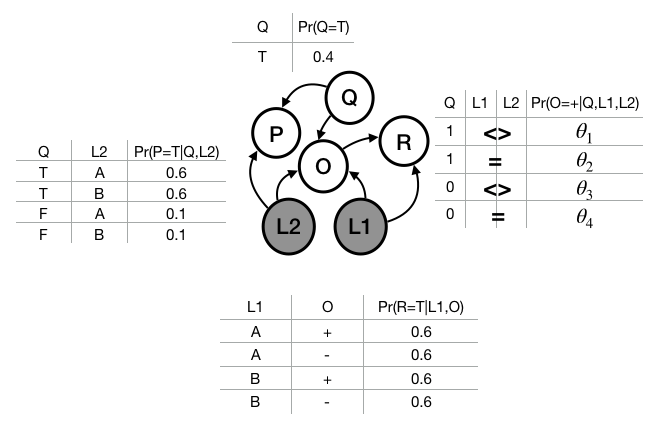
\includegraphics[width=\textwidth]{figs/BN.png}
  \end{minipage}\hfill
  \begin{minipage}[c]{0.45\textwidth}
    \caption{
        \small The model used for generating the datasets. There are four binary random variables, P, Q, O, and R. \textbf{P}: indicates whether or not the employee has high performance; \textbf{Q}: indicates whether or not an employee has high qualification; \textbf{O}: indicates whether or not the colleague submits the positive opinion towards the employee;  \textbf{R}: indicates whether or not the colleague has a positive opinion towards the employee;  \textbf{L1, L2}: indicates the label of the review provider and review receiver (observed).
    } \label{fig:BN}
  \end{minipage}
\end{figure}

We show the effectiveness of FairPSL by performing an empirical evaluation. We investigate two research questions in our experiments:
\begin{description}
\item[Q1] What is the effect of the fairness threshold $\delta$ on the fairness measures $RD/RC/RR$?
\item[Q2] How is decision quality affected by imposing $\delta$-fairness constraints?
\end{description}

Note that although we present the result for specific parameters of the framework in this section, we ran extensive analysis and the results we present are representative. We implemented the MAP inference routines of PSL and FairPSL in Python, using Gurobi-8.1\footnote{\url{www.gurobi.com}} as the backend solver. The FairPSL code, code for the data generator and data is publicly available\footnote{https://github.com/gfarnadi/FairPSL}. 

\subsection{Data generation}
  
We evaluate the FairPSL inference algorithm on synthetic datasets representing the performance review scenario (introduced in Example~\ref{ex:review}). The organization hierarchy is generated synthetically. 
The organization hierarchy generator is parameterized by two numbers: the number of employees in the organization ($n$) and the number of employees managed by each manager ($k$). Each employee is randomly assigned with a label \emph{A} or \emph{B}. An examples organization hierarchy with $n$=50 and $k$=3 is shown in Figure~\ref{fig:hierachy}.

\begin{figure}
  \begin{minipage}[c]{0.3\textwidth}
    \caption{
        \small An example of an organizational hierarchy with five levels and 50 employees with k=3. Each employee either has label A (shown with grey) or B (shown with white).
    }\label{fig:hierachy} 
	\end{minipage} \hfill
    \begin{minipage}[c]{0.7\textwidth}
    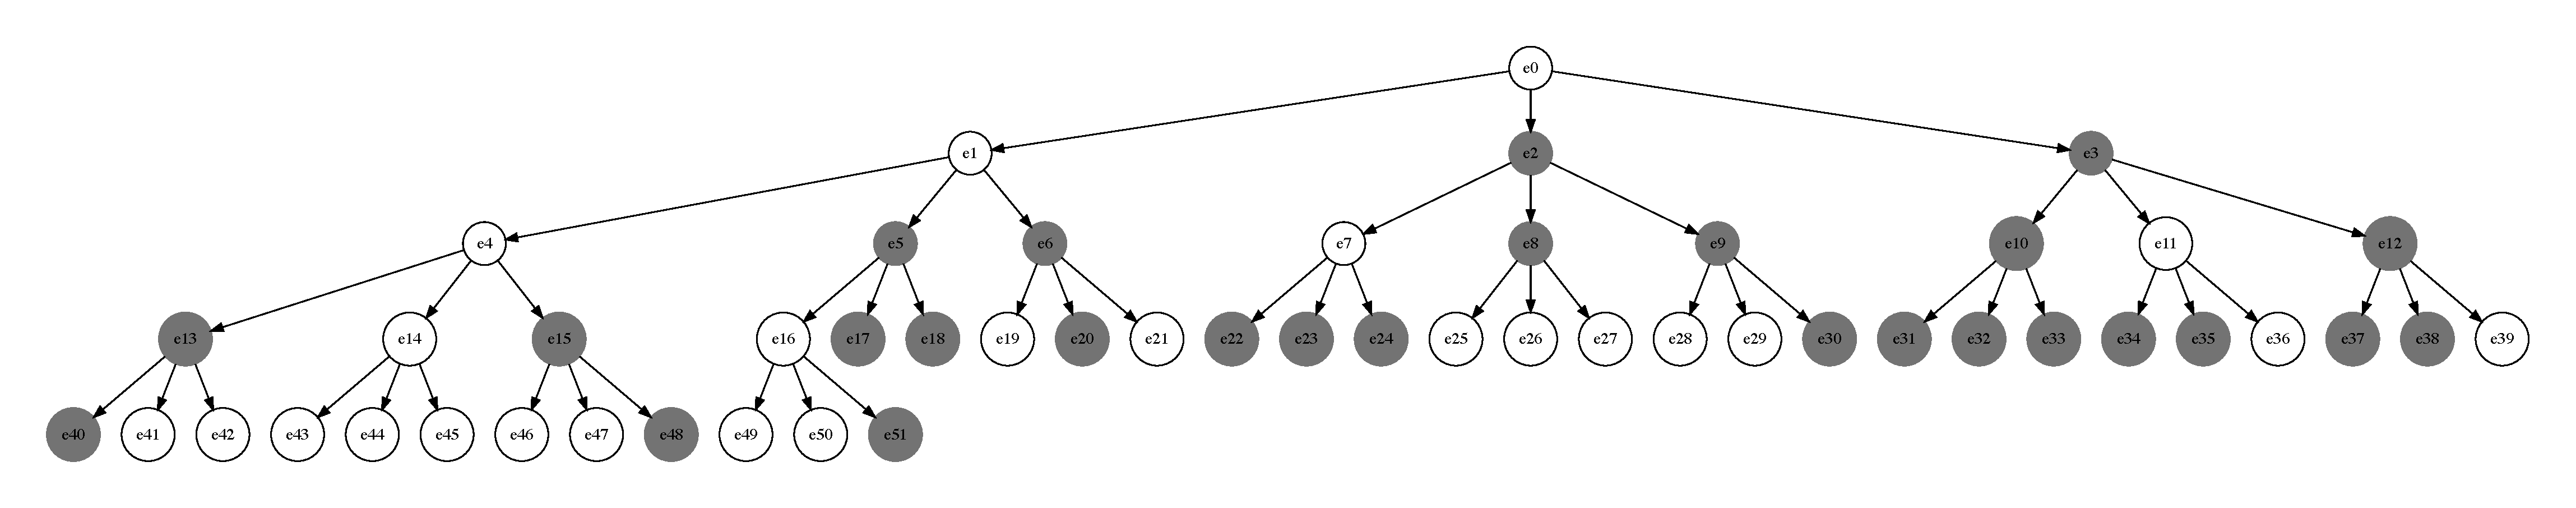
\includegraphics[width=\textwidth]{figs/Uni-hierachy.pdf}
  \end{minipage}
\end{figure}

For each employee, we use the generative model of Figure~\ref{fig:BN} to draw assignments for all the random variables. We assume that only $40\%$ of employees are qualified for promotion and regardless of their labels, employees submit only $60\%$ of their opinions. In addition, due to various personal and environmental factors, only $60\%$ of high quality employees perform well while $10\%$ of low quality employees also perform well regardless of their labels. Note that these numbers are not specific and just chosen for the framework to serve as a representative setting and a proof of concept. The conditional probability table for the opinion variable $O$ is parameterized by four values $(\theta_1, \theta_2, \theta_3, \theta_4)$ which together determine the degree of discrimination against the protected group. Since other parameters in the Bayesian network did not have a direct effect on the degree of discrimination, we fixed them to arbitrary values. 

The results presented in this section are based on an organization hierarchy  with $100$ employees where $k=5$. However, the results of the framework are not sensitive to the settings as we test the framework with various organization sizes ranging from $50$ to $500$ employees and various degree for $k$ ranging from $3$ to $10$. We generated seven datasets given the organization hierarchy using different values for the $\theta$ parameters: $(0.0,1.0,0.0,0.0)$, $(0.33,1.0,0.0,0.0)$, $(0.66,1.0,0.0,0.0)$, $(1.0,1.0,0.0,0.0)$, $(1.0,1.0,0.0,0.33)$, $(1.0,1.0,0.0,0.66)$, $(1.0,1.0,0.0,1.0)$. 
 
In the first three settings the discrimination originates from negative opinions towards qualified outgroup employees. The first setup is an extreme case where the opinion towards outgroup employees is always negative. The discrimination in the last three settings originates from positive opinions towards unqualified ingroup employees. The last setup is an extreme case where the opinion towards ingroup employees is always positive. The fourth setup represent unbiased opinions where employees are treated similarly based on their qualification. 

\paragraph{MAP Inference} We use the model presented in Table~\ref{tab:pslmodel} for MAP inference in PSL and FairPSL (recall that in FairPSL, the $\delta$-fairness constraints corresponding to one of the fairness measures are also added to the model). The observed atoms are $\textit{Manager(m,e)}$, $\textit{PositiveReview(e1,e2)}$ and labels of all employees. The truth values for all other atoms are obtained via MAP inference. We use the truth values obtained for the decision atoms $\textit{ToPromote(e)}$ to compute the fairness measures. We defined the discriminative pattern, and the protected and unprotected groups of this problem in Section~\ref{sec:formulation}.


\subsection{Evaluation results}

\begin{figure}
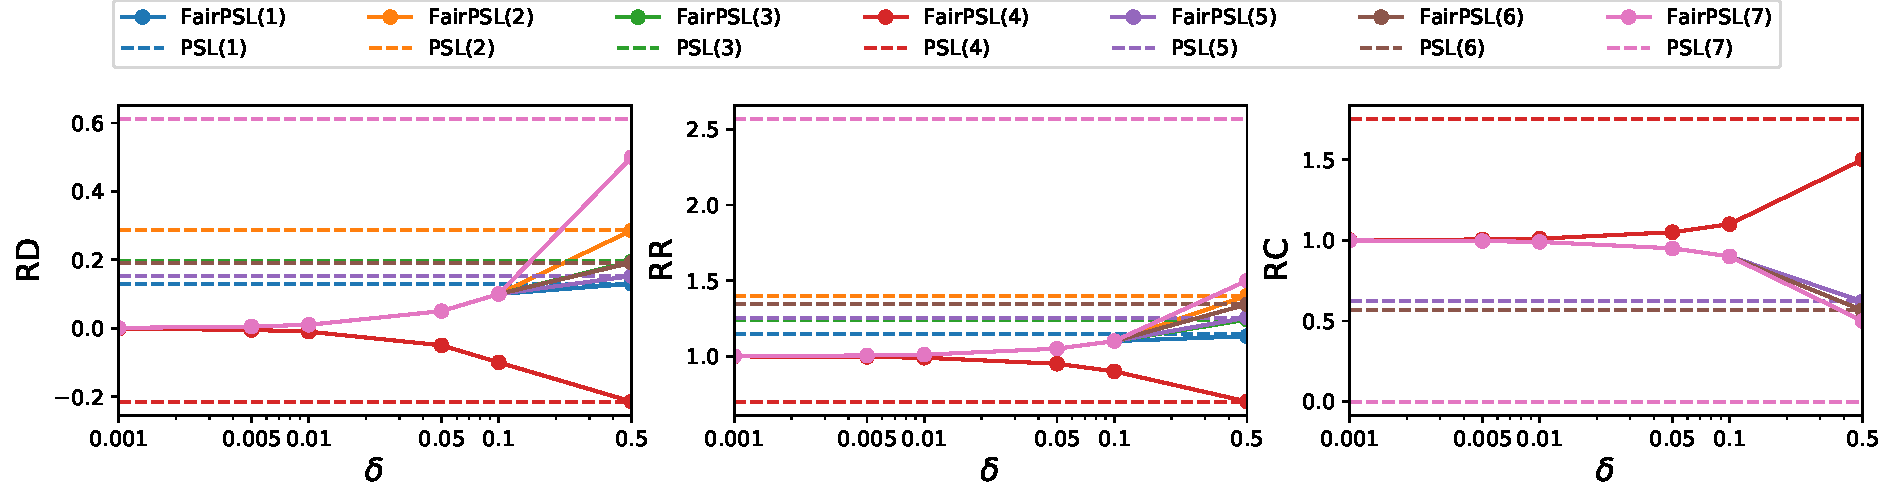
\includegraphics[width=1\linewidth]{figs/results_vis_uni_params.pdf}
\caption{\small Fairness score of predictions obtained by MAP inference of PSL and FairPSL, according to the fairness measures \emph{RD}, \emph{RR}, and \emph{RC}. The labels of datasets are mentioned with parenthesis next to the inference method. The FairPSL values of each measure are obtained by adding the $\delta$-fairness constraint of that measure.\label{fig:results}
}  
\end{figure}

To answer \textbf{Q1}, we run the MAP inference algorithm of PSL and FairPSL on seven synthetic datasets. 
We run the MAP inference of FairPSL multiple times on each dataset: For each of the three fairness measures, we add the corresponding $\delta$-fairness constraint with five thresholds $\{0.001, 0.005, 0.01, 0.05, 0.1, 0.5\}$.

Figure~\ref{fig:results} shows the fairness score of predictions in terms of the three fairness measures. As expected, tighter $\delta$-fairness constraints lead to better scores. Note that the best possible score according to RD is 0, as it computes a difference. Since RR and RC compute ratios, the best possible score according to these measures is 1. In our experiments, with any of these measures, taking $\delta = 0.001$ pushes the score of predictions to its limit.  

The $\delta$-fairness constraints modify the optimization problem of MAP inference by reducing the feasible region to solutions that conform with fairness guarantees. Research question \textbf{Q2} is concerned with the effect of this reduction on the accuracy of predictions. Note that decision quality is the same as the accuracy of predictions. To answer this question, we compare the inferred values for the decision atoms \textit{ToPromote(e)} against their actual values. These values are extracted from the known values of \textit{IsQualified(e)} according to rules 11 and 12 in Table~\ref{tab:pslmodel}. Figure~\ref{fig:accuracy} shows the area under the curve of the receiver operating characteristic~(AUC) of predicting the decision variable in three groups, namely the protected group, the unprotected group (i.e., promotion of the employees who have in-group managers), and all employees. By doing so, we make sure that our fairness constraints do not propagate bias towards either of the populations. Since the results of FairPSL with $\delta$-fairness constraints RR and RC are very similar to the results of RD, we only report the latter here.


\begin{figure}
    \centering
    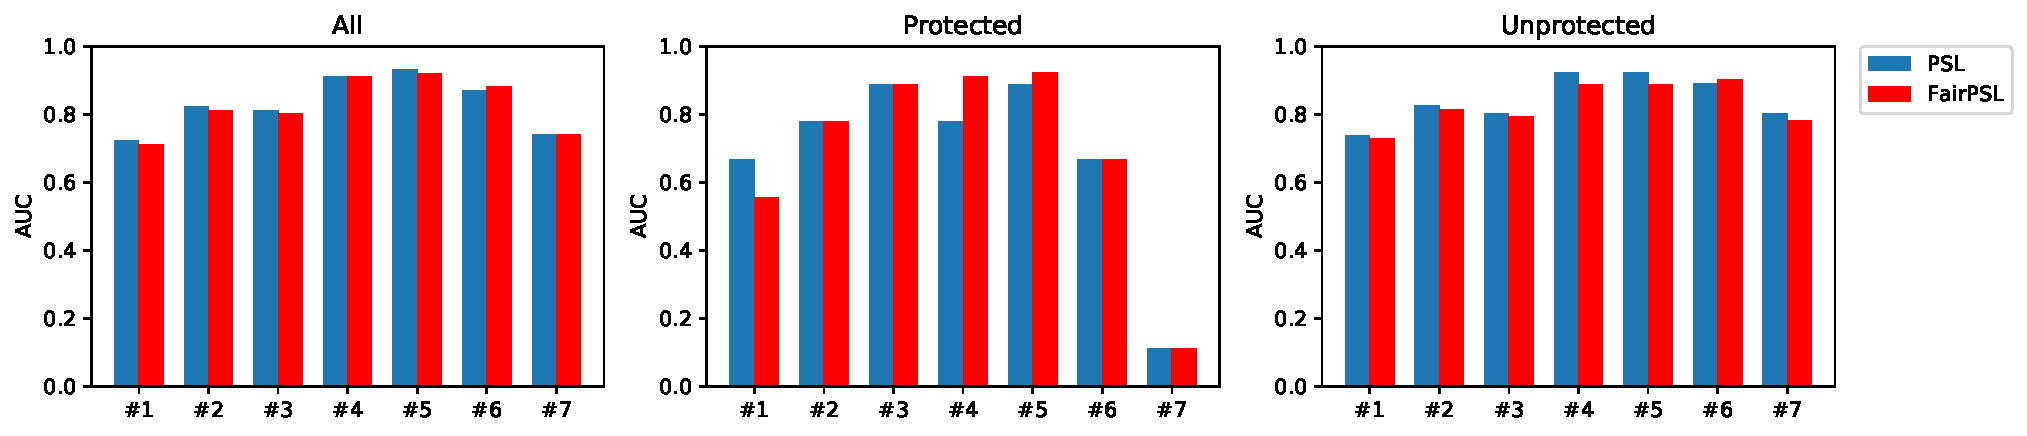
\includegraphics[width=\textwidth]{figs/roc.pdf}
    \caption{\small AUC score of predictions for truth values of unknown atoms \textit{ToPromote(e)} using MAP inference of PSL and FairPSL with $\delta$-fairness constraints $RD$ with $\delta=0.001$.}
    \label{fig:accuracy}
\end{figure}

According to Figure~\ref{fig:accuracy}, the results of both PSL and FairPSL in all seven datasets are close to each other. Note that although fairness may impose a cost in terms of overall accuracy, FairPSL often improves the accuracy of the protected class. Sometimes the overall predictions of FairPSL are even slightly better than PSL (e.g., dataset 6 and 7). As expected, the accuracy of the fourth setting where the opinions are unbiased are similar in both PSL and FairPSL. We observe that prediction of MAP inference for both FairPSL and PSL are similar, thus, in these settings at least, FairPSL guarantees fairness without hurting accuracy. Further investigation is required on the effect of the various ranges of discrimination (i.e., $\theta_1$, $\theta_2$, $\theta_3$, $\theta_4$) on the prediction results of FairPSL.



We also generate various types of organizations in which labels are not uniformly distributed, e.g., one population only occurs at the bottom levels of an organization. While we did not observe any differences in the behavior of our method with respect to accuracy and fairness measure, we found that the degree of discrimination is higher in such organizations. Further investigations on the structure of an organization on discrimination is an interesting direction for future research. 

\section{Conclusion and Future Directions}
\label{sec:conclusion}
Many applications of AI and machine learning affect peoples' lives in important ways. While there is a growing body of work on fairness in AI and ML, it assumes an individualistic notion of fairness.   In this paper, we have proposed a general framework for relational fairness which includes both a rich language for defining discrimination patterns and an efficient algorithm for performing inference subject to fairness constraints. We show our approach enforces fairness guarantees while preserving the accuracy of the predictions. 

There are many avenues for expanding on this work. For example, here we assumed that the discriminative pattern is given, however an automatic mechanism to extract discriminatory situations hidden in a large amount of decision records is an important and required task. Discrimination discovery has been studied for attribute-based fairness~\cite{pedreschi2013discovery}. An interesting next step is discrimination pattern discovery in relational data.

\section*{Acknowledgements}
This work is supported by the National Science Foundation under Grant Numbers CCF-1740850 and IIS-1703331. Golnoosh Farnadi and Behrouz Babaki are  supported by postdoctoral scholarships from IVADO through the Canada First Research Excellence Fund (CFREF) grant.

\begin{thebibliography}{10}
\itemsep=1pt 
\begin{small}

\bibitem{EUlaw}
European union legislation. (a) racial equality directive, 2000; (b) employment
  equality directive, 2000; (c) gender employment directive, 2006; (d) equal
  treatment directive (proposal), 2008.

\bibitem{UKlaw}
{UK} legislation. (a) sex discrimination act, 1975, (b) race relation act,
  1976.

\bibitem{USlaw}
United nations legislation. (a) universal declaration of human rights, 1948,
  (c) convention on the elimination of all forms of racial discrimination,
  1966, (d) convention on the elimination of all forms of discrimination
  against women, 1979.

\bibitem{alshukaili:iswc16}
Duhai Alshukaili, Alvaro A.~A. Fernandes, and Norman~W. Paton.
\newblock Structuring linked data search results using probabilistic soft
  logic.
\newblock In {\em International Semantic Web Conference {(1)}}, volume 9981 of
  {\em Lecture Notes in Computer Science}, pages 3--19, 2016.

\bibitem{bach:jmlr17}
Stephen~H. Bach, Matthias Broecheler, Bert Huang, and Lise Getoor.
\newblock Hinge-loss markov random fields and probabilistic soft logic.
\newblock {\em Journal of Machine Learning Research}, 18:109:1--109:67, 2017.

\bibitem{barocas2016big2}
Solon Barocas and Andrew~D Selbst.
\newblock Big data's disparate impact.
\newblock {\em California Law Review}, 104:671, 2016.

\bibitem{boyd2014networked}
Danah Boyd, Karen Levy, and Alice Marwick.
\newblock The networked nature of algorithmic discrimination.
\newblock In {\em Data and discrimination: Collected essays}, pages 53--57.
  2014.

\bibitem{brewer1979group}
Marilynn~B Brewer.
\newblock In-group bias in the minimal intergroup situation: A
  cognitive-motivational analysis.
\newblock {\em Psychological bulletin}, 86(2):307, 1979.

\bibitem{brewer2007social}
Marilynn~B Brewer.
\newblock The social psychology of intergroup relations: Social categorization,
  ingroup bias, and outgroup prejudice.
\newblock {\em Social Psychology: Handbook of Basic Principles}, 2007.

\bibitem{chouldechova2017fair2}
Alexandra Chouldechova.
\newblock Fair prediction with disparate impact: {A} study of bias in
  recidivism prediction instruments.
\newblock {\em CoRR}, abs/1703.00056, 2017.

\bibitem{dwork2012fairness3}
Cynthia Dwork, Moritz Hardt, Toniann Pitassi, Omer Reingold, and Richard~S.
  Zemel.
\newblock Fairness through awareness.
\newblock In {\em {ITCS}}, pages 214--226. {ACM}, 2012.

\bibitem{ebrahimi:emnlp16}
Javid Ebrahimi, Dejing Dou, and Daniel Lowd.
\newblock Weakly supervised tweet stance classification by relational
  bootstrapping.
\newblock In {\em {EMNLP}}, pages 1012--1017. The Association for Computational
  Linguistics, 2016.

\bibitem{farnadi2018fairness}
Golnoosh Farnadi, Behrouz Babaki, and Lise Getoor.
\newblock Fairness in relational domains.
\newblock In {\em AAAI/ACM Conference on AI, Ethics, and Society (AIES)}, pages
  108--114. ACM, 2018.

\bibitem{feldman2015certifying2}
Michael Feldman, Sorelle~A. Friedler, John Moeller, Carlos Scheidegger, and
  Suresh Venkatasubramanian.
\newblock Certifying and removing disparate impact.
\newblock In {\em {KDD}}, pages 259--268. {ACM}, 2015.

\bibitem{getoor2007introduction}
Lise Getoor and Ben Taskar.
\newblock {\em {Introduction to Statistical Relational Learning}}.
\newblock MIT press Cambridge, 2007.

\bibitem{hardt2016equality3}
Moritz Hardt, Eric Price, and Nati Srebro.
\newblock Equality of opportunity in supervised learning.
\newblock In {\em {NIPS}}, pages 3315--3323, 2016.

\bibitem{kamishima2011fairness}
Toshihiro Kamishima, Shotaro Akaho, and Jun Sakuma.
\newblock Fairness-aware learning through regularization approach.
\newblock In {\em ICDMW}, pages 643--650. {IEEE} Computer Society, 2011.

\bibitem{kouki:recsys15}
Pigi Kouki, Shobeir Fakhraei, James~R. Foulds, Magdalini Eirinaki, and Lise
  Getoor.
\newblock Hyper: {A} flexible and extensible probabilistic framework for hybrid
  recommender systems.
\newblock In {\em RecSys}, pages 99--106. {ACM}, 2015.

\bibitem{counterfactualfairness}
Matt~J. Kusner, Joshua~R. Loftus, Chris Russell, and Ricardo Silva.
\newblock Counterfactual fairness.
\newblock In {\em {NIPS}}, pages 4069--4079, 2017.

\bibitem{Pedreschi:2012}
Dino Pedreschi, Salvatore Ruggieri, and Franco Turini.
\newblock A study of top-k measures for discrimination discovery.
\newblock In {\em {SAC}}, pages 126--131. {ACM}, 2012.

\bibitem{pedreschi2013discovery}
Dino Pedreschi, Salvatore Ruggieri, and Franco Turini.
\newblock The discovery of discrimination.
\newblock In {\em Discrimination and Privacy in the Information Society},
  volume~3 of {\em Studies in Applied Philosophy, Epistemology and Rational
  Ethics}, pages 91--108. Springer, 2013.

\bibitem{ridgeway2004unpacking}
Cecilia~L Ridgeway and Shelley~J Correll.
\newblock Unpacking the gender system: A theoretical perspective on gender
  beliefs and social relations.
\newblock {\em Gender \& society}, 18(4):510--531, 2004.

\bibitem{sridhar:bioinformatics16}
Dhanya Sridhar, Shobeir Fakhraei, and Lise Getoor.
\newblock A probabilistic approach for collective similarity-based drug-drug
  interaction prediction.
\newblock {\em Bioinformatics}, 32(20):3175--3182, 2016.

\bibitem{verma2018fairness2}
Sahil Verma and Julia Rubin.
\newblock Fairness definitions explained.
\newblock In {\em 2018 IEEE/ACM International Workshop on Software Fairness
  (FairWare)}, pages 1--7. IEEE, 2018.

\bibitem{west2014exploiting}
Robert West, Hristo~S. Paskov, Jure Leskovec, and Christopher Potts.
\newblock Exploiting social network structure for person-to-person sentiment
  analysis.
\newblock {\em {TACL}}, 2:297--310, 2014.

\bibitem{zafar2017parity}
Muhammad~Bilal Zafar, Isabel Valera, Manuel Gomez{-}Rodriguez, Krishna~P.
  Gummadi, and Adrian Weller.
\newblock From parity to preference-based notions of fairness in
  classification.
\newblock In {\em {NIPS}}, pages 228--238, 2017.

\bibitem{zemel2013learning}
Richard~S. Zemel, Yu~Wu, Kevin Swersky, Toniann Pitassi, and Cynthia Dwork.
\newblock Learning fair representations.
\newblock In {\em {ICML} {(3)}}, volume~28 of {\em {JMLR} Workshop and
  Conference Proceedings}, pages 325--333. JMLR.org, 2013.

\end{small}
\end{thebibliography}

\end{document}

\end{article}



\end{articlesection}

% put the news items below- there can be multiple news sections
% each with its own title
% news will usually have an author as well as a title, 
% e.g. TCDE elections
% news articles are in the same format as letters
% typically, news articles will be stored in a directory called "news"

%\begin{newssection}{News headline}

% insert news items here; news will typically have authors
% see the Sept. 2018 issue for an example

%\begin{news}{news item title}
%{author name}{author affiliation}
%\input{news/news-article.tex}
%\end{news}
%
%\newpage


%\end{newssection}



\begin{callsection}

%  This section will be empty for your version
%
%  Calls for papers section.  Use the callsection environment.
%  Each call for papers is contained in an call environment, where the single 
%  required options to \begin{call} is the name of the conference.
% typically calls are stored in a "calls" directory
%
%\begin{call}{name of conference}
%\centerline{\includegraphics[width=\textwidth, bb= 0 0 590 760]{calls/conference-name.pdf}}
%\end{call}
%\begin{call}{ICDE 2019 Conference}
%\centerline{
\includegraphics[width=\textwidth, bb= 0 0 610 790] {../Dec-2018/calls/icde19.pdf}} 
%\centerline{
\includegraphics[width=\textwidth, bb= 0 0 590 760] {calls/icde19.pdf}}
%\end{call}
\begin{call}{TCDE Membership Form}
%\centerline{\includegraphics[width=\textwidth, bb= 0 0 610 790]
\centerline{
\includegraphics[width=\textwidth, bb= 0 0 590 760] {../Dec-2018/calls/tcde.pdf}}
\end{call}

\end{callsection}

\end{bulletin}
\end{document}
